%package list
\documentclass{article}
\usepackage[top=3cm, bottom=3cm, outer=3cm, inner=3cm]{geometry}
\usepackage{multicol}
\usepackage{graphicx}
\usepackage{url}
%\usepackage{cite}
\usepackage{hyperref}
\usepackage{array}
%\usepackage{multicol}
\newcolumntype{x}[1]{>{\centering\arraybackslash\hspace{0pt}}p{#1}}
\usepackage{natbib}
\usepackage{pdfpages}
\usepackage{multirow}
\usepackage[normalem]{ulem}
\useunder{\uline}{\ul}{}
\usepackage{svg}
\usepackage{xcolor}
\usepackage{listings}
\lstdefinestyle{ascii-tree}{
    literate={├}{|}1 {─}{--}1 {└}{+}1 
  }
\lstset{basicstyle=\ttfamily,
  showstringspaces=false,
  commentstyle=\color{red},
  keywordstyle=\color{blue}
}
%\usepackage{booktabs}
\usepackage{caption}
\usepackage{subcaption}
\usepackage{float}
\usepackage{array}

\usepackage{enumitem}


\newcolumntype{M}[1]{>{\centering\arraybackslash}m{#1}}
\newcolumntype{N}{@{}m{0pt}@{}}


%%%%%%%%%%%%%%%%%%%%%%%%%%%%%%%%%%%%%%%%%%%%%%%%%%%%%%%%%%%%%%%%%%%%%%%%%%%%
%%%%%%%%%%%%%%%%%%%%%%%%%%%%%%%%%%%%%%%%%%%%%%%%%%%%%%%%%%%%%%%%%%%%%%%%%%%%
\newcommand{\itemEmail}{vmaldonadov@unsa.edu.pe}
\newcommand{\itemStudent}{Victor Gonzalo Maldonado Vilca}
\newcommand{\itemCourse}{Programación Web 2}
\newcommand{\itemCourseCode}{1702122}
\newcommand{\itemSemester}{III}
\newcommand{\itemUniversity}{Universidad Nacional de San Agustín de Arequipa}
\newcommand{\itemFaculty}{Facultad de Ingeniería de Producción y Servicios}
\newcommand{\itemDepartment}{Departamento Académico de Ingeniería de Sistemas e Informática}
\newcommand{\itemSchool}{Escuela Profesional de Ingeniería de Sistemas}
\newcommand{\itemAcademic}{2024 - A}
\newcommand{\itemInput}{Del 9 de abril de 2024}
\newcommand{\itemOutput}{Al 18 de mayo de 2024}
\newcommand{\itemPracticeNumber}{04}
\newcommand{\itemTheme}{Ajax}
%%%%%%%%%%%%%%%%%%%%%%%%%%%%%%%%%%%%%%%%%%%%%%%%%%%%%%%%%%%%%%%%%%%%%%%%%%%%
%%%%%%%%%%%%%%%%%%%%%%%%%%%%%%%%%%%%%%%%%%%%%%%%%%%%%%%%%%%%%%%%%%%%%%%%%%%%

\usepackage[english,spanish]{babel}
\usepackage[utf8]{inputenc}
\AtBeginDocument{\selectlanguage{spanish}}
\renewcommand{\figurename}{Figura}
\renewcommand{\refname}{Referencias}
\renewcommand{\tablename}{Tabla} %esto no funciona cuando se usa babel
\AtBeginDocument{%
	\renewcommand\tablename{Tabla}
}

\usepackage{fancyhdr}
\pagestyle{fancy}
\fancyhf{}
\setlength{\headheight}{30pt}
\renewcommand{\headrulewidth}{1pt}
\renewcommand{\footrulewidth}{1pt}
\fancyhead[L]{\raisebox{-0.2\height}{
\includegraphics[width=3cm]{img/logo_episunsa.png}}}
\fancyhead[C]{\fontsize{7}{7}\selectfont	\itemUniversity \\ \itemFaculty \\ \itemDepartment \\ \itemSchool \\ \textbf{\itemCourse}}
\fancyhead[R]{\raisebox{-0.2\height}{
\includegraphics[width=1.2cm]{img/logo_abet}}}
\fancyfoot[L]{Victor M.}
\fancyfoot[C]{\itemCourse}
\fancyfoot[R]{Página \thepage}

% para el codigo fuente
\usepackage{listings}
\usepackage{color, colortbl}
\definecolor{dkgreen}{rgb}{0,0.6,0}
\definecolor{gray}{rgb}{0.5,0.5,0.5}
\definecolor{mauve}{rgb}{0.58,0,0.82}
\definecolor{codebackground}{rgb}{0.95, 0.95, 0.92}
\definecolor{tablebackground}{rgb}{0.8, 0, 0}

\lstset{frame=tb,
	language=bash,
	aboveskip=3mm,
	belowskip=3mm,
	showstringspaces=false,
	columns=flexible,
	basicstyle={\small\ttfamily},
	numbers=none,
	numberstyle=\tiny\color{gray},
	keywordstyle=\color{blue},
	commentstyle=\color{dkgreen},
	stringstyle=\color{mauve},
	breaklines=true,
	breakatwhitespace=true,
	tabsize=3,
	backgroundcolor= \color{codebackground},
}

\begin{document}
	
	\vspace*{10px}
	
	\begin{center}	
		\fontsize{17}{17} \textbf{ Informe de Laboratorio 04}
	\end{center}
	\centerline{\textbf{\Large Tema: \itemTheme}}
	%\vspace*{0.5cm}	

	\begin{flushright}
		\begin{tabular}{|M{2.5cm}|N|}
			\hline 
			\rowcolor{tablebackground}
			\color{white} \textbf{Nota}  \\
			\hline 
			     \\[30pt]
			\hline 			
		\end{tabular}
	\end{flushright}	

	\begin{table}[H]
		\begin{tabular}{|x{4.7cm}|x{4.8cm}|x{4.8cm}|}
			\hline 
			\rowcolor{tablebackground}
			\color{white} \textbf{Estudiante} & \color{white}\textbf{Escuela}  & \color{white}\textbf{Asignatura}   \\
			\hline 
			{\itemStudent \par \itemEmail} & \itemSchool & {\itemCourse \par Semestre: \itemSemester \par Código: \itemCourseCode}     \\
			\hline 			
		\end{tabular}
	\end{table}		
	
	\begin{table}[H]
		\begin{tabular}{|x{4.7cm}|x{4.8cm}|x{4.8cm}|}
			\hline 
			\rowcolor{tablebackground}
			\color{white}\textbf{Tarea} & \color{white}\textbf{Tema}  & \color{white}\textbf{Duración}   \\
			\hline 
			\itemPracticeNumber & \itemTheme & 2 horas   \\
			\hline 
		\end{tabular}
	\end{table}
	
	\begin{table}[H]
		\begin{tabular}{|x{4.7cm}|x{4.8cm}|x{4.8cm}|}
			\hline 
			\rowcolor{tablebackground}
			\color{white}\textbf{Semestre académico} & \color{white}\textbf{Fecha de inicio}  & \color{white}\textbf{Fecha de entrega}   \\
			\hline 
			\itemAcademic & \itemInput &  \itemOutput  \\
			\hline 
		\end{tabular}
	\end{table}
	

%%%%%%%%%%%%%%%%%%%%
 
	\section{Tarea}
	\textbf{Ejercicios Propuestos:}
	\begin{itemize}		
		\item Revisar Ajax en w3schools y Presentar un informe con un pantallazo por cada ejemplo de Ajax realizado en su propio servidor web.
		\item Usar un servidor web como apache en su computadora (Xampp), descargar el archivo de datos data.json y dejarlo en el mismo lugar donde lanzó el servidor. \textbf{Para cada uno de estos problemas implemente un programa en ajax y página que:}
		\begin{itemize}
			\item Liste todas las “regiones”. 
			\item Muestre el número total de confirmados por región.
			\item Encuentre las 10 regiones cuya suma total sea la mayor.
			\item Visualice un gráfico en el tiempo de los valores para la región de Arequipa.
			\item Haga gráficos comparativos entre regiones usando líneas.
			\item Visualice un gráfico comparativo del crecimiento en regiones excepto Lima y Callao.
			\item Haga gráficos comparativos entre regiones elegidas por el usuario.
			\item Visualice un gráfico comparativo del crecimiento en regiones excepto Lima y Callao, mostrando el número de confirmados por cada día.
		\end{itemize}
		\item En grupos de 3 a 5 personas (los grupos se definirán en clase) implemente una aplicación web que navegue sobre archivos Markdown y permita:
		\begin{itemize}
			\item Listar los archivos Markdown disponibles.
			\item Ver el contenido de un archivo markdown traducido a HTML.
			\item Crear nuevos archivos MarkDown y almacenarlos en el servidor
		\end{itemize}
		\textbf{Tener en cuenta:}
		\begin{itemize}
			\item La comunicación entre el cliente y el servidor tiene que ser usando JSON sólamente.
			\item El cliente debe usar AJAX para sus peticiones.
			\item El servidor debe usar NodeJS.
			\item Su aplicación debe ser de página única, es decir que sólo habrá un archivo index.html y nada más.
		\end{itemize}
			
	\end{itemize}
 
    \section{Entregables}
    \begin{itemize}
        \item Informe de trabajo
        \item URL: Repositorio de GitHub
    \end{itemize}
    
		
	\section{Equipos, materiales y temas utilizados}
	\begin{itemize}
		\item HTML
		\item CSS
		\item JavaScript
		\item w3schools
		\item Xampp
		\item Node.js
		\item Ajax
        \item GitHub
	\end{itemize}
 
	
	\section{URL de Repositorio Github}
	\begin{itemize}
		\item URL del Repositorio GitHub para clonar o recuperar.
		\item \url{https://github.com/Victor-Gonzalo-Maldonado-Vilca/TareaAjax.git}
	\end{itemize}
	\section{Link de Video}
	\begin{itemize}
		\item URL video en Youtube.
		\item \url{https://www.youtube.com/watch?v=tPlgxQkUKaY}
	\end{itemize}

%%%%%%%%%%%%%%%%%%%%


    \section{Desarrollo del trabajo}
    \subsection{AJAX w3schools - EXAMPLES}
    Capturas de pantalla de los ejemplos de Ajax, usando su propio servidor.
    \newpage
    \begin{itemize}
    	\item \textbf{Tutorial JavaScript sección Ajax}
    	\begin{figure}[H]
    		\centering
    		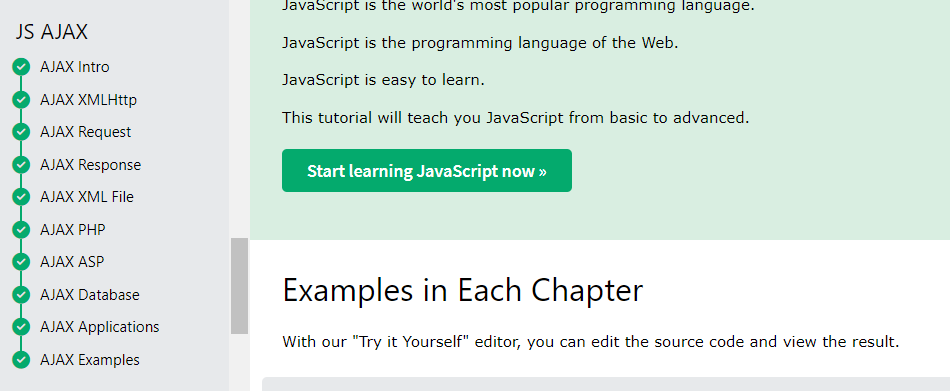
\includegraphics[width=1\textwidth,keepaspectratio]{img/w3schools.png}
    		\caption{w3schools}
    	\end{figure}
    \end{itemize}

%%%%%%%%%%%%%%%%%%%%
	\subsubsection{AJAX - Intro}
	\begin{itemize}
		\item \textbf{AJAX Example}
		\begin{figure}[H]
			\centering
			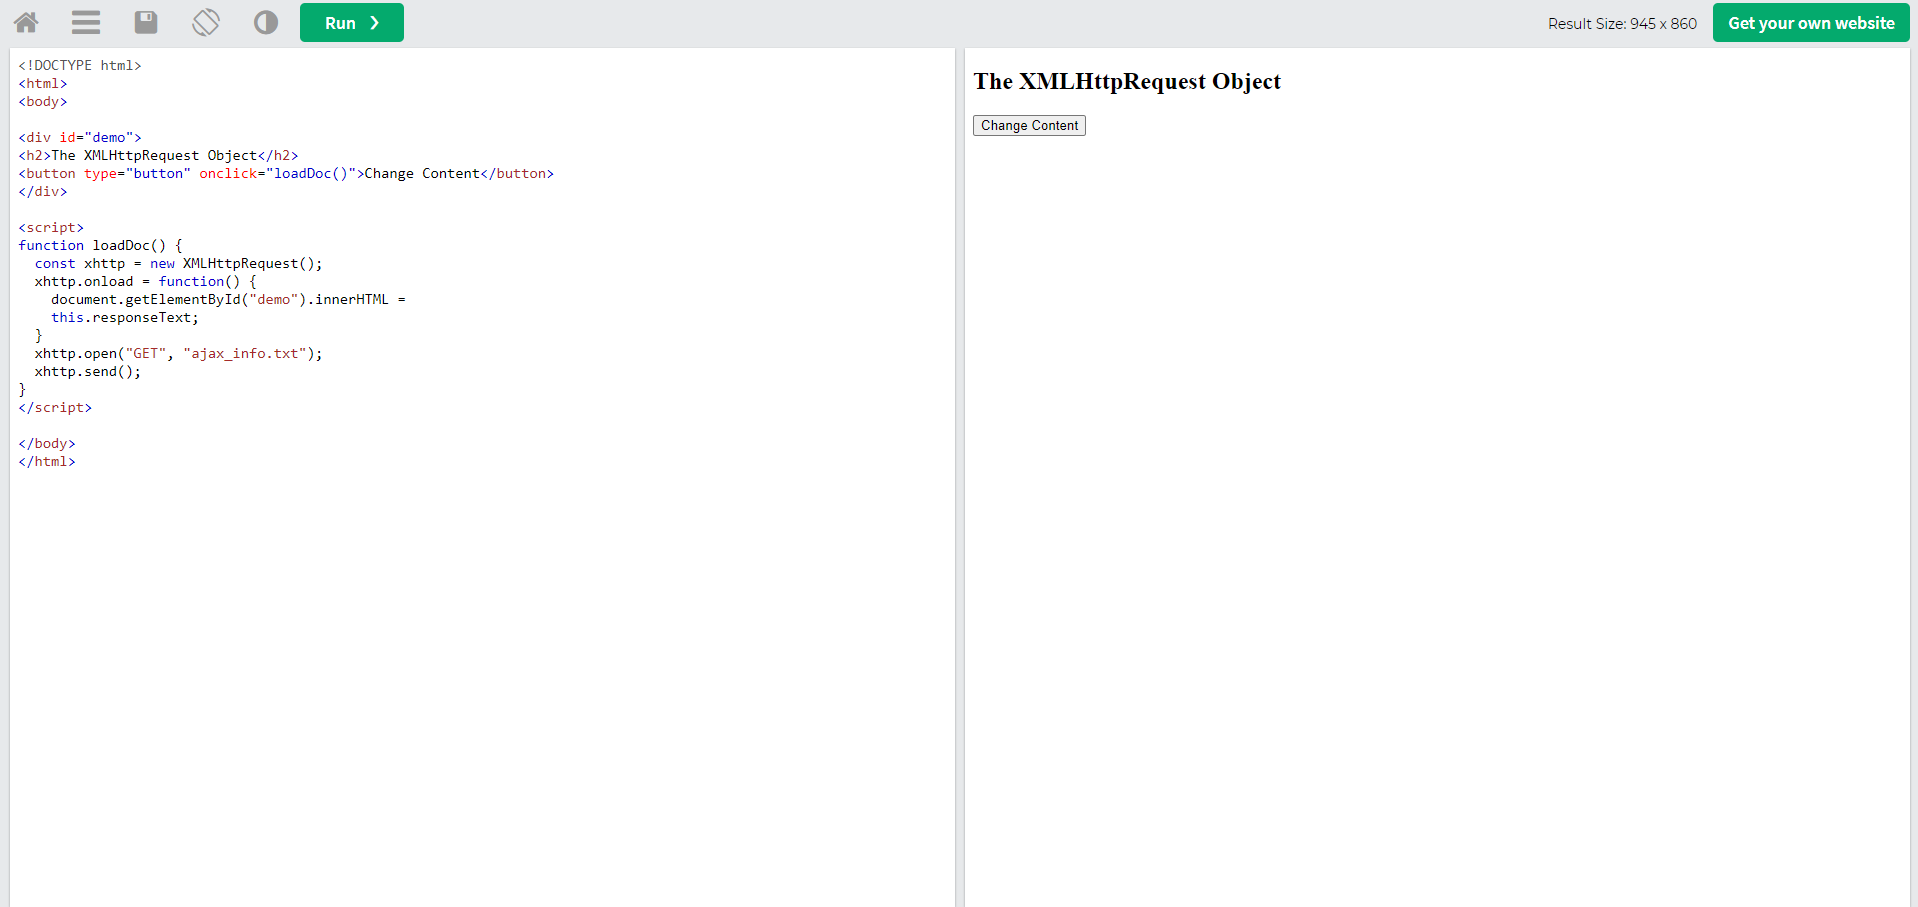
\includegraphics[width=1\textwidth,keepaspectratio]{img/ejemplo0.png}
			\caption{AJAX}
		\end{figure}
		\newpage
		\begin{figure}[H]
			\centering
			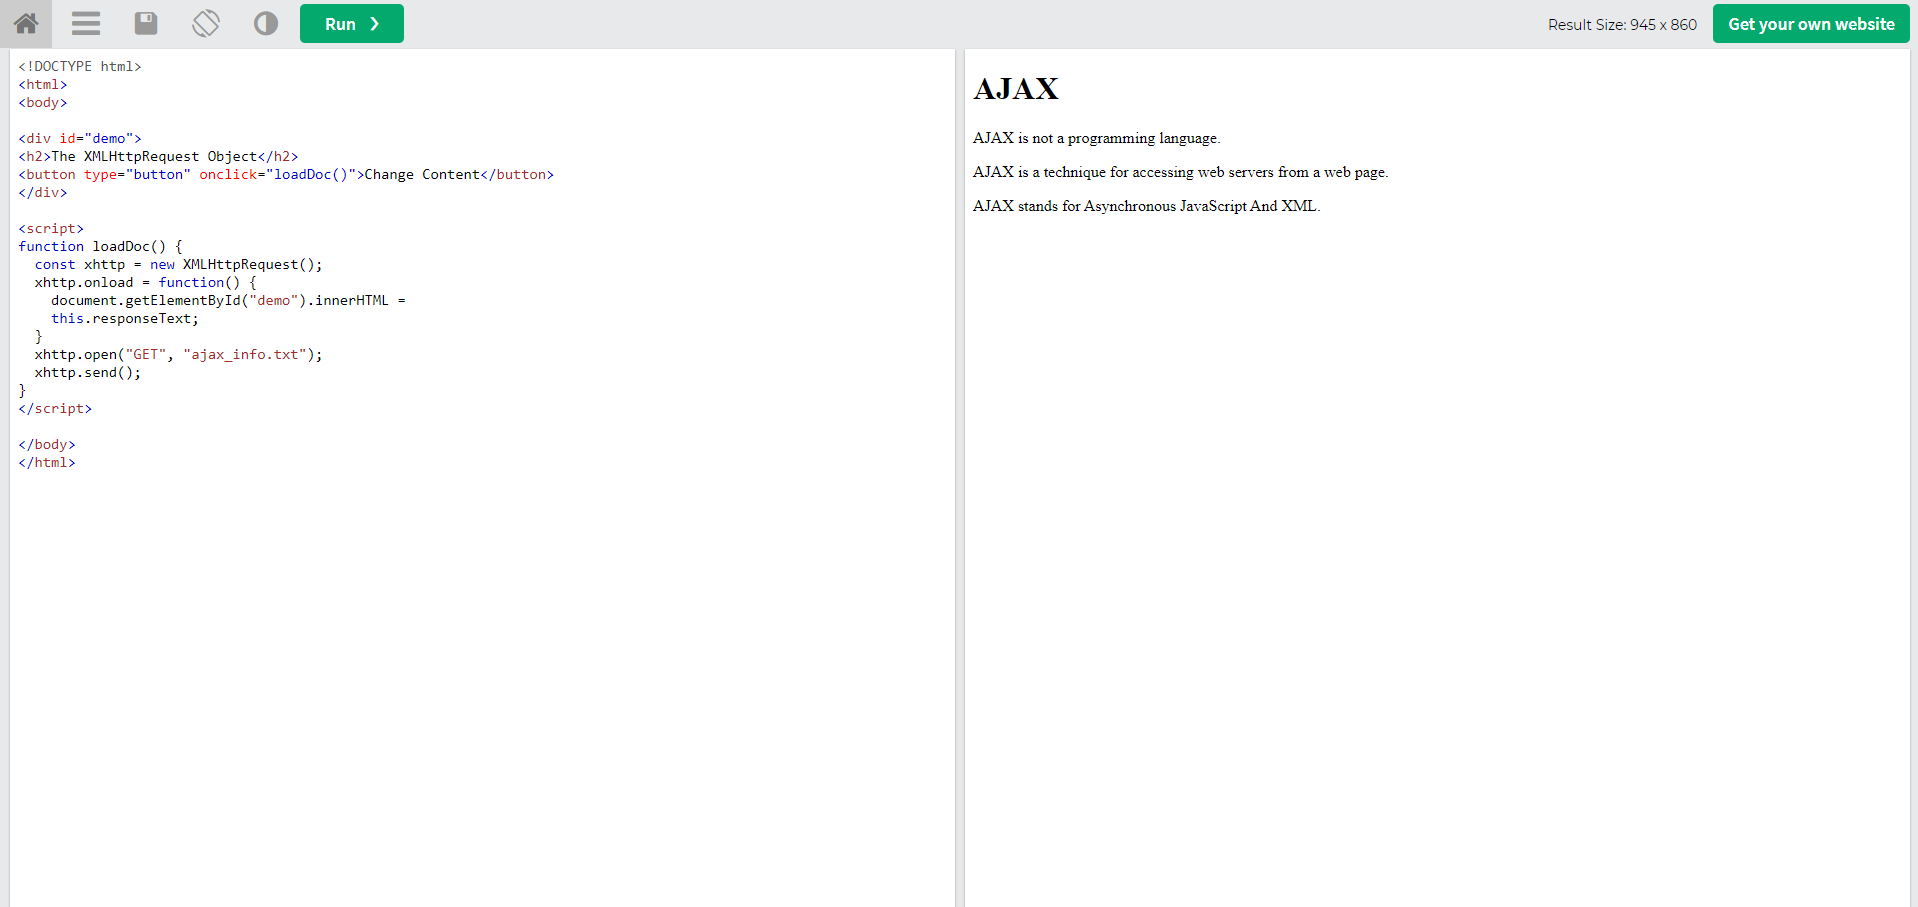
\includegraphics[width=1\textwidth,keepaspectratio]{img/boton0.png}
			\caption{Presionando el botón}
		\end{figure}
	\end{itemize}
%%%%%%%%%%%%%%%%%%%%
    \subsubsection{AJAX - XMLHttp}
    \begin{itemize}
    	\item \textbf{Ejemplo 1 - Enviar una Solicitud:}
    	\begin{figure}[H]
    		\centering
    		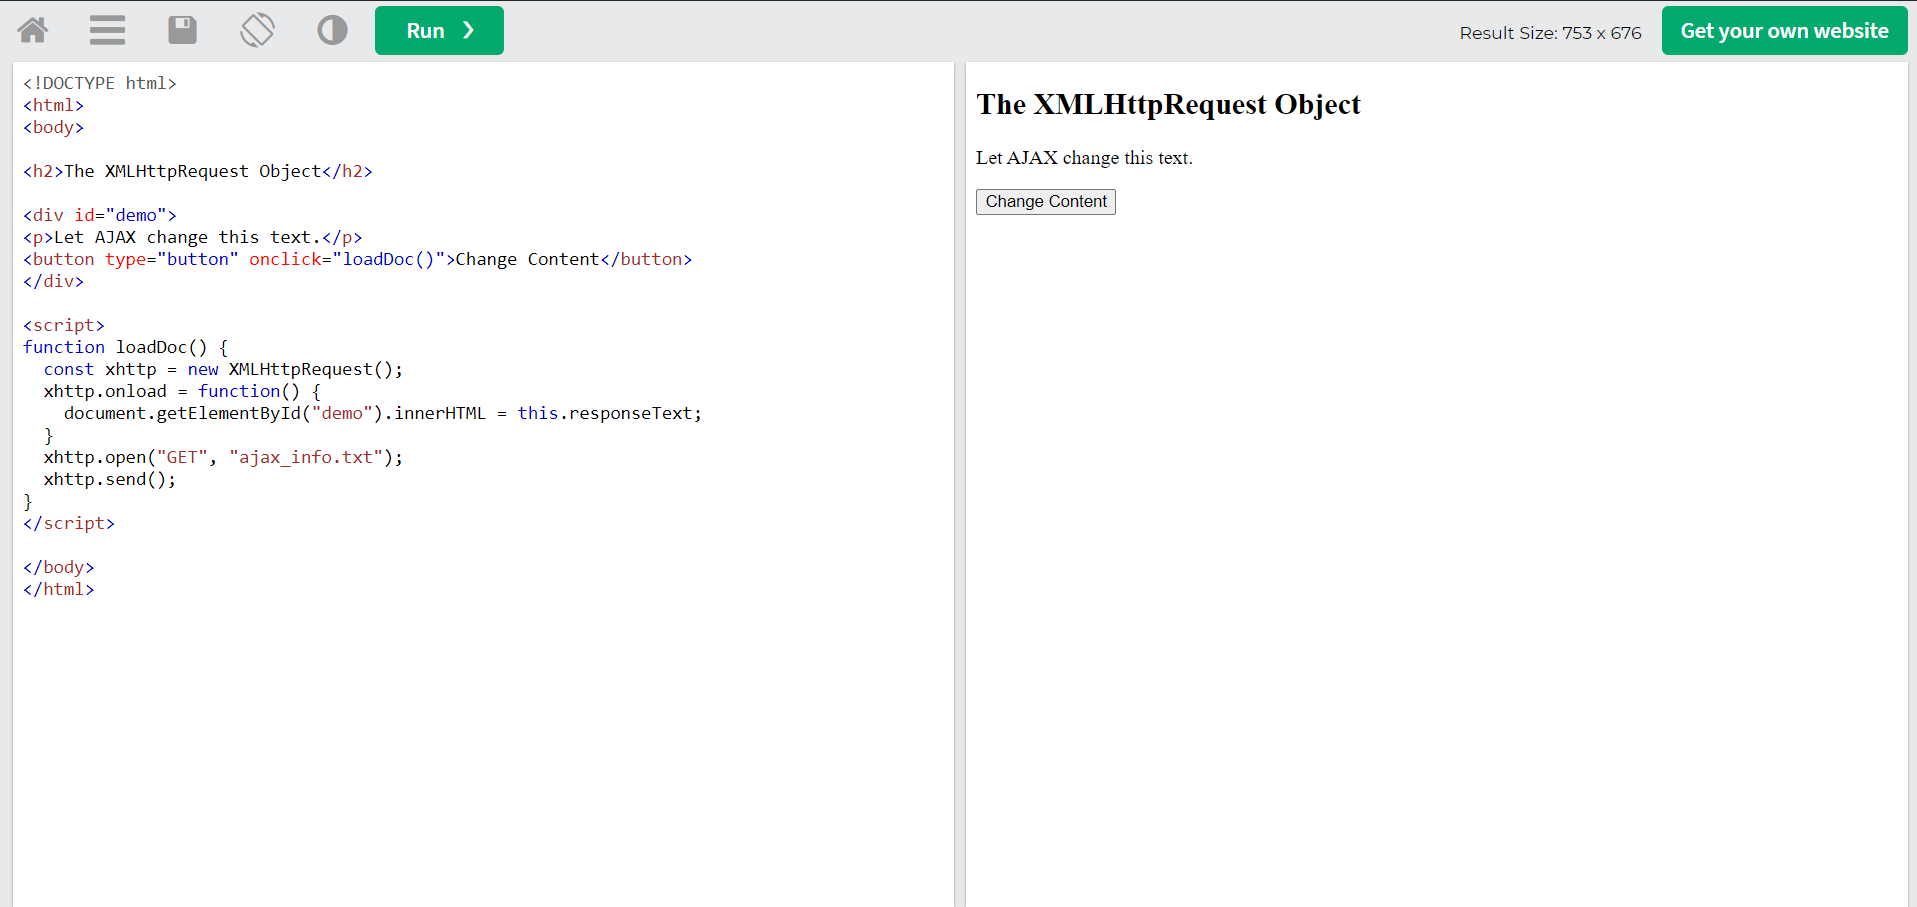
\includegraphics[width=1\textwidth,keepaspectratio]{img/ejemplo1.png}
    		\caption{Enviar Solicitud}
    	\end{figure}
    	\begin{figure}[H]
    		\centering
    		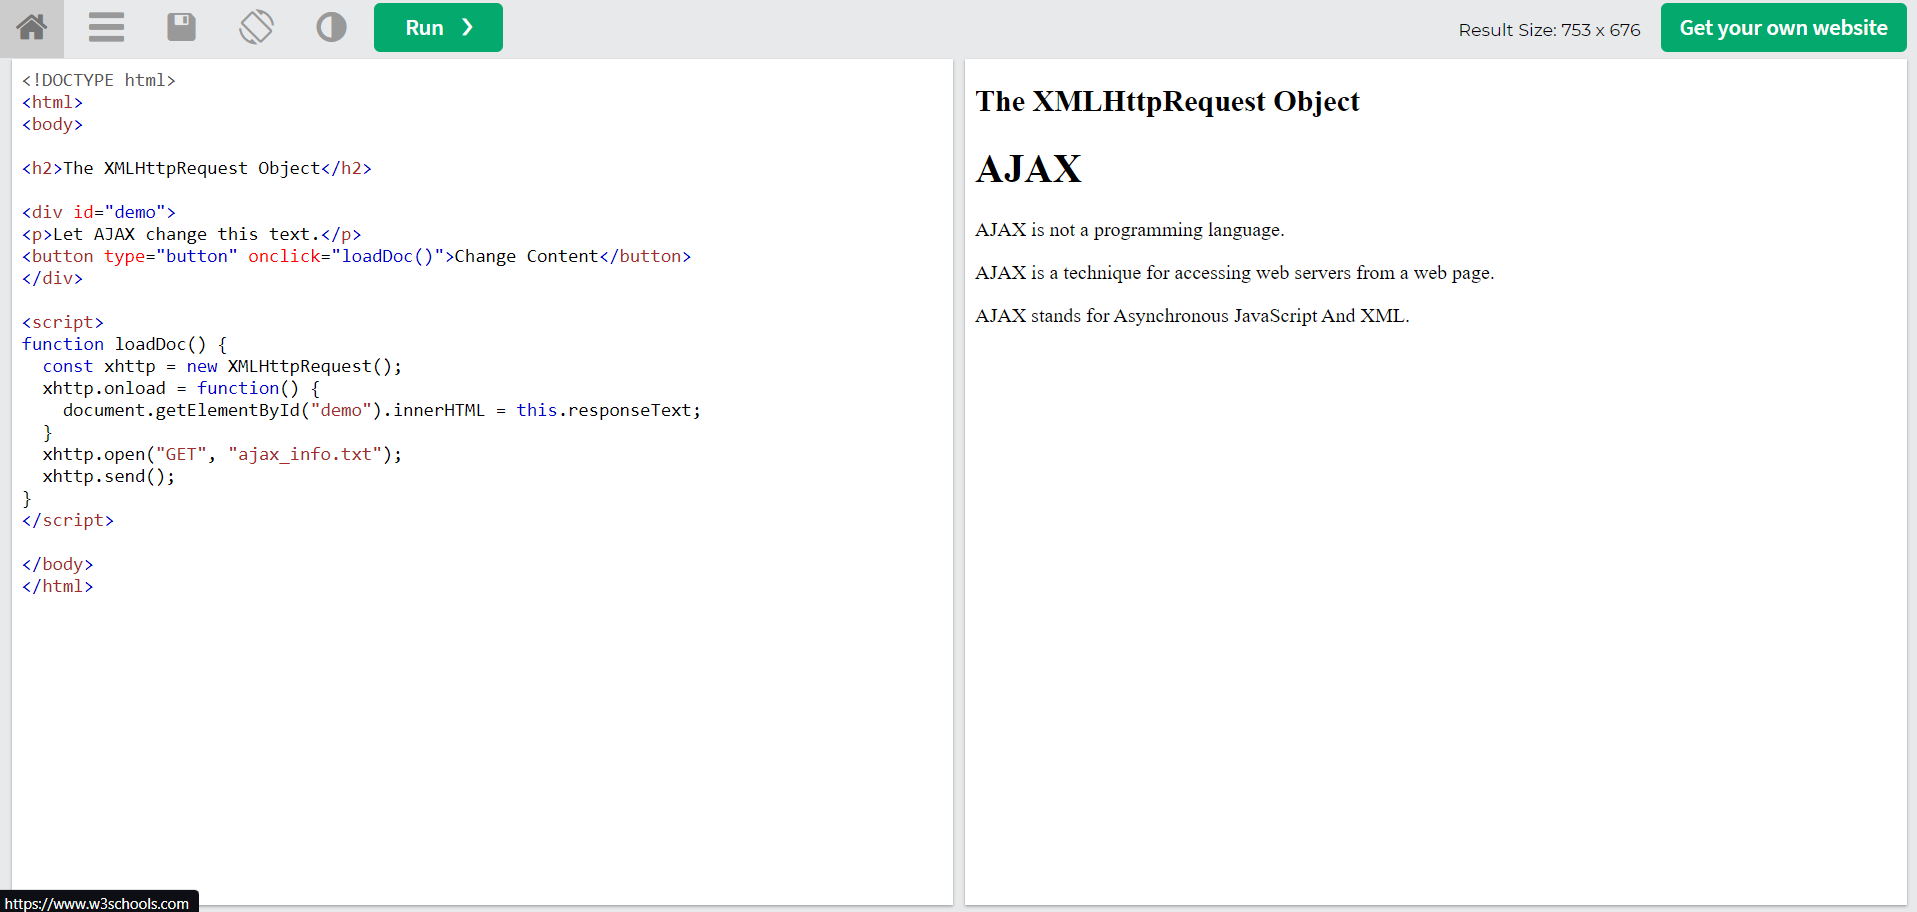
\includegraphics[width=1\textwidth,keepaspectratio]{img/boton1.png}
    		\caption{Presionando el botón}
    	\end{figure}
    	\item \textbf{Ejemplo 2 - Propiedad de carga:}
    	\begin{figure}[H]
    		\centering
    		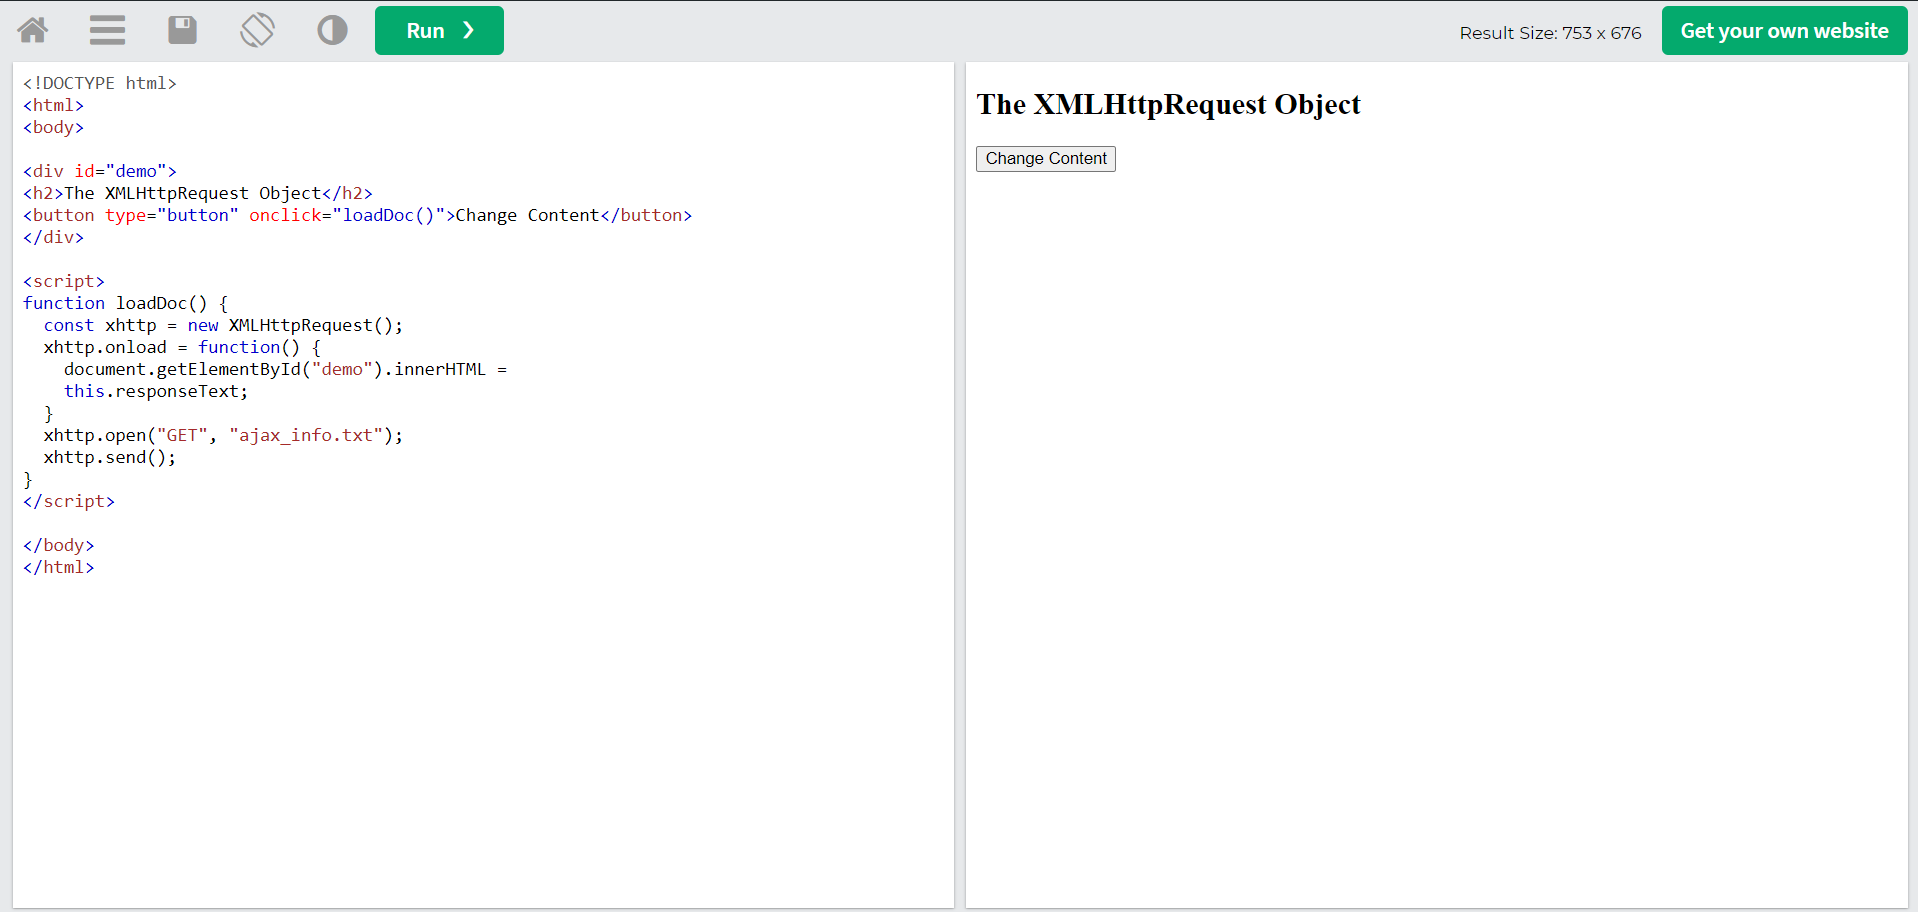
\includegraphics[width=1\textwidth,keepaspectratio]{img/ejemplo2.png}
    		\caption{Propiedad de Carga}
    	\end{figure}
    	\newpage
    	\begin{figure}[H]
    		\centering
    		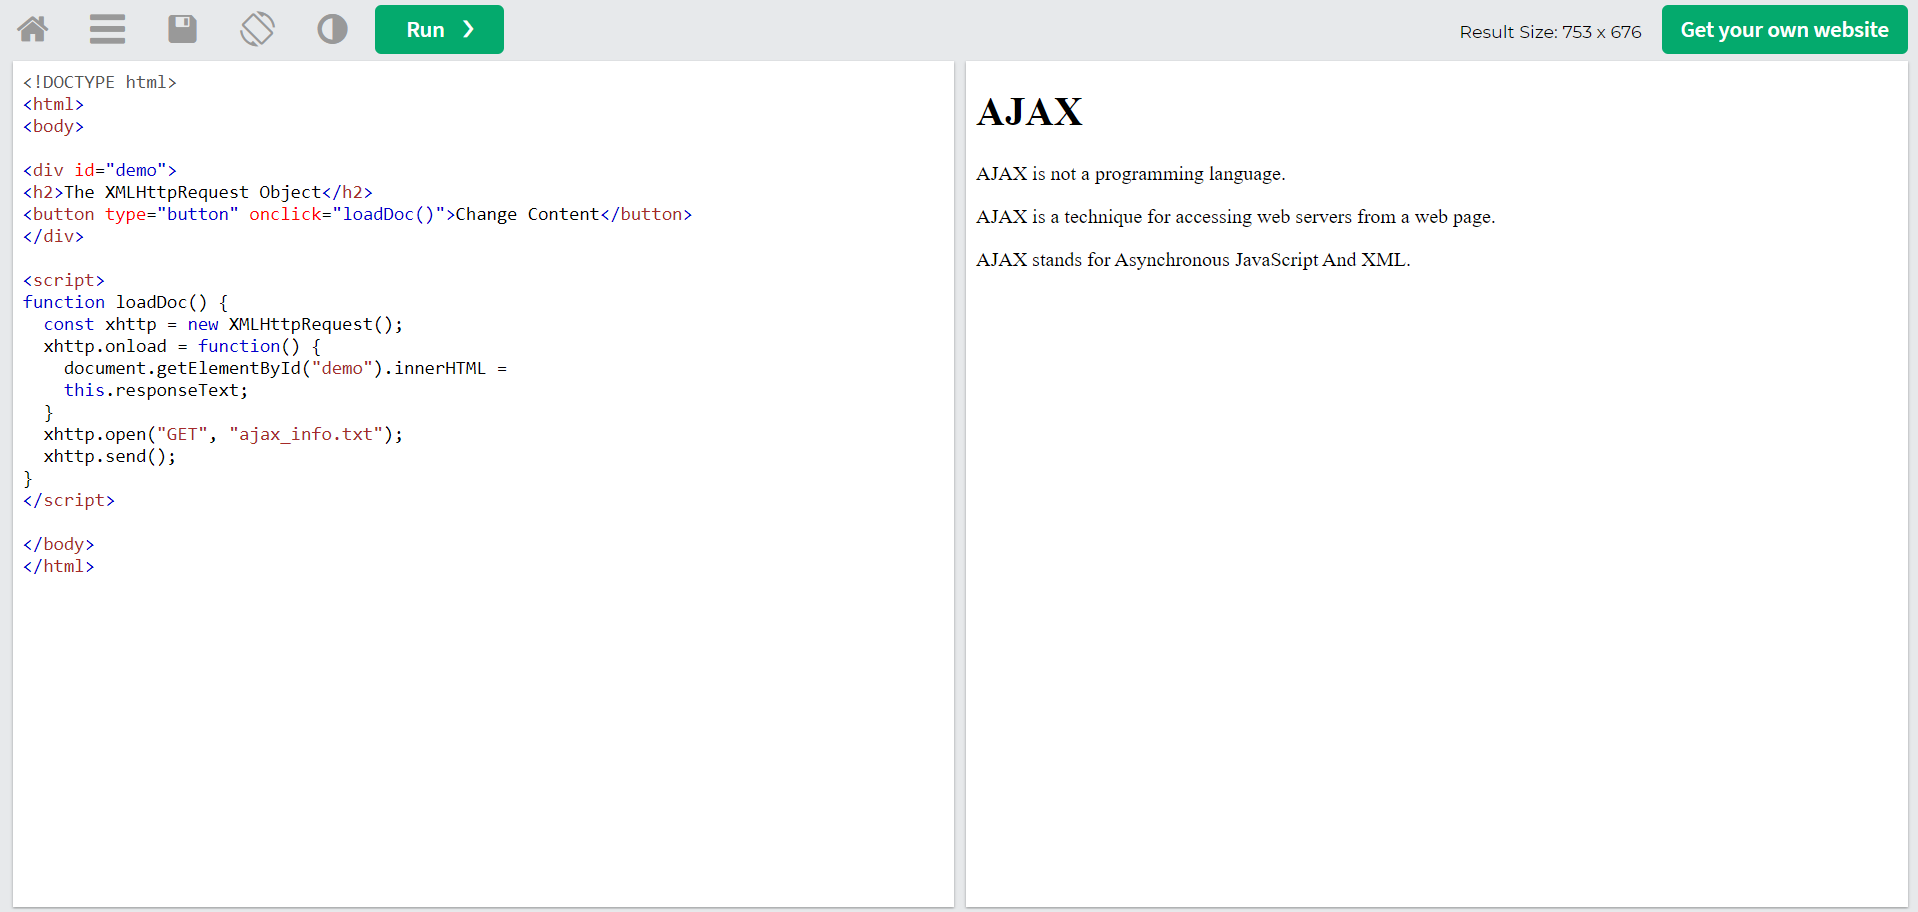
\includegraphics[width=1\textwidth,keepaspectratio]{img/boton2.png}
    		\caption{Presionando el botón}
    	\end{figure}
    	\item \textbf{Ejemplo 3 - Propiedad Onreadystatechange: }
    	\begin{figure}[H]
    		\centering
    		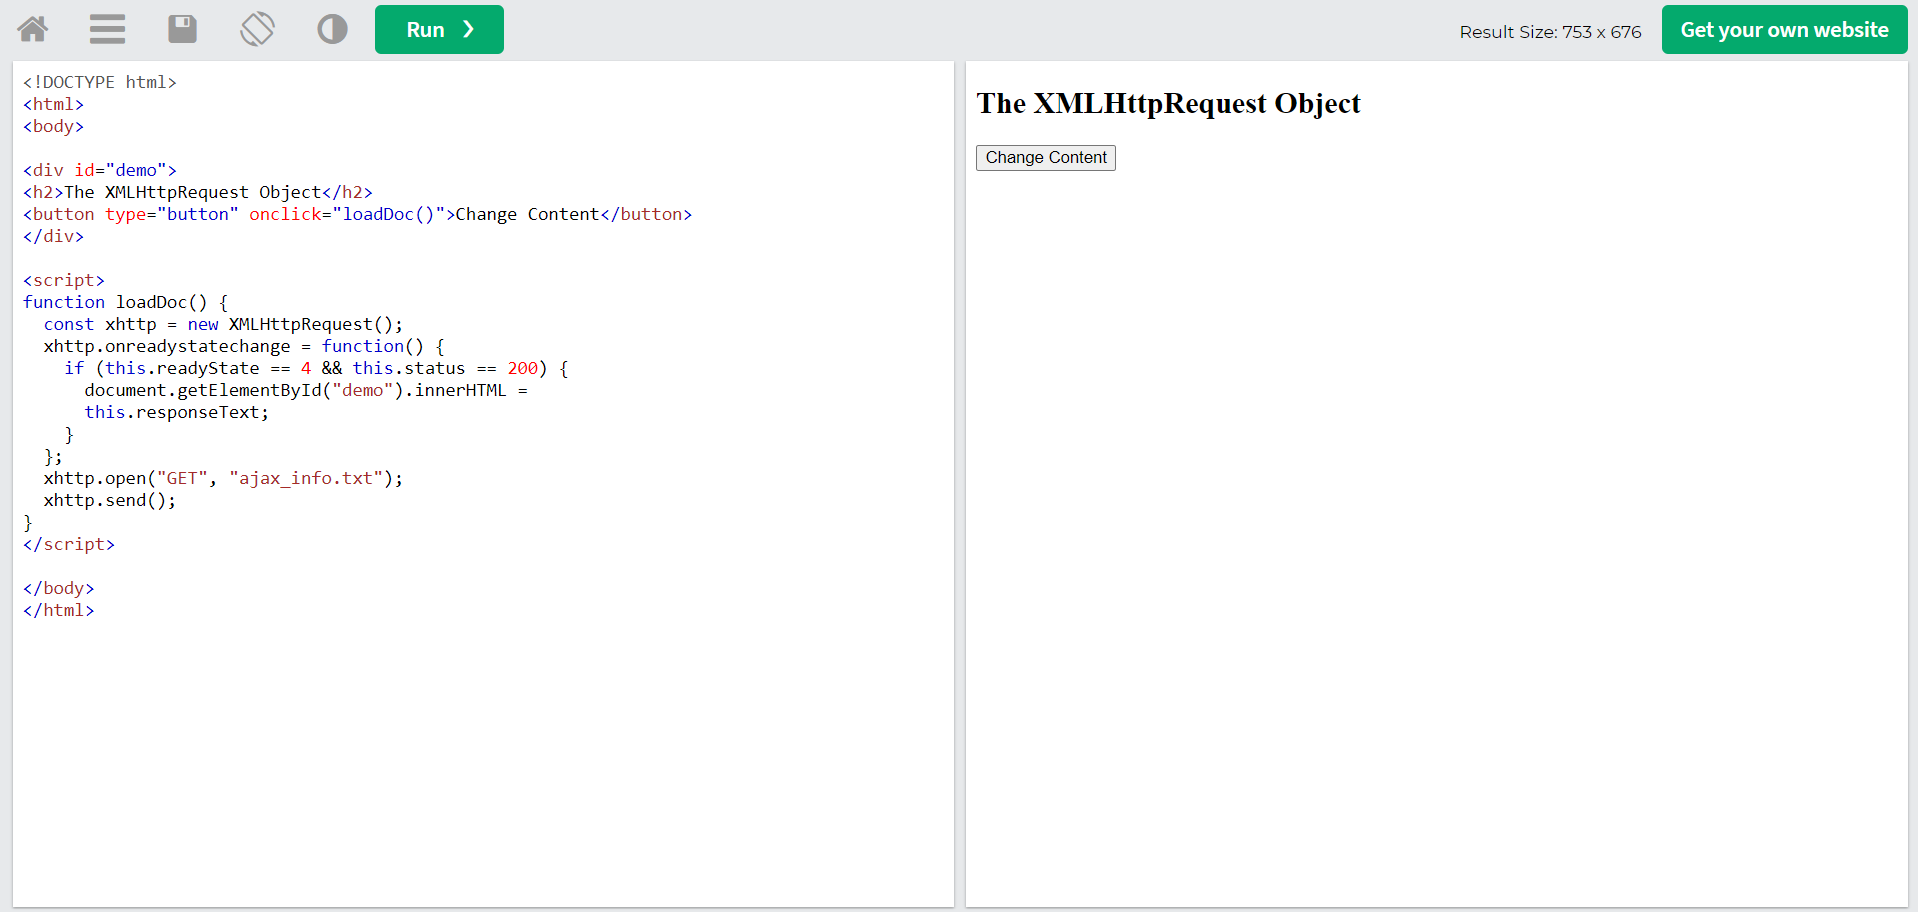
\includegraphics[width=1\textwidth,keepaspectratio]{img/ejemplo3.png}
    		\caption{Propiedad Onreadystatechange}
    	\end{figure}
    	\begin{figure}[H]
    		\centering
    		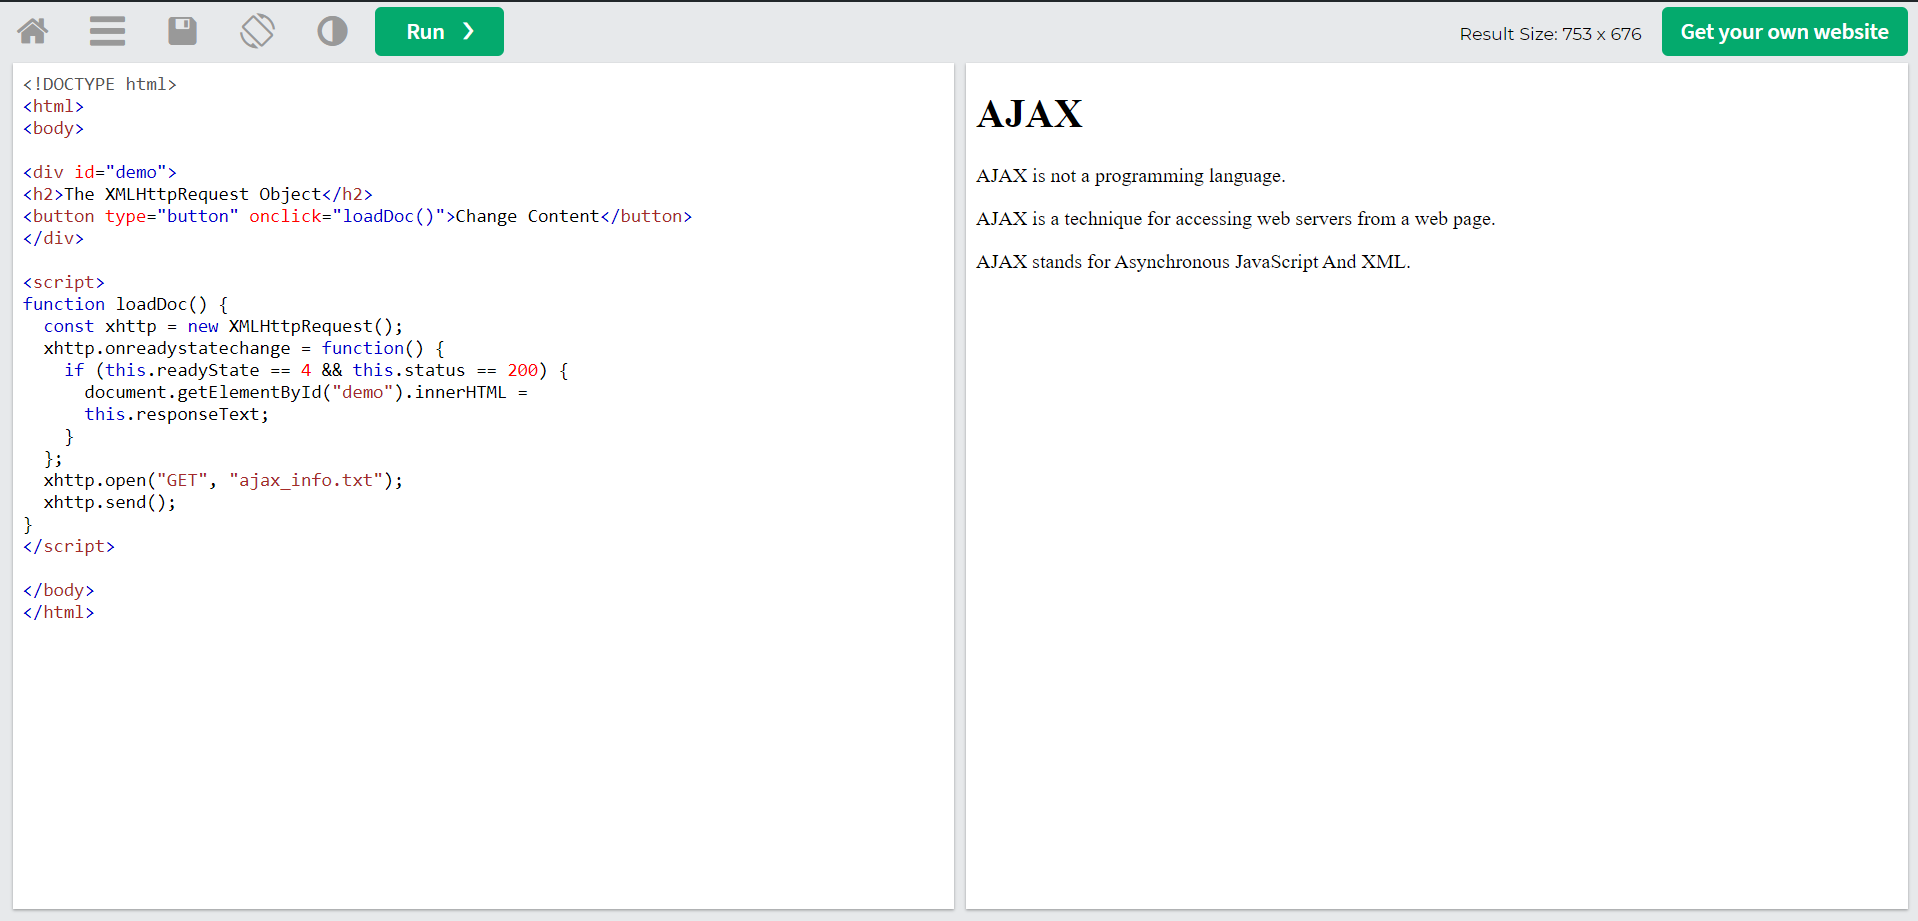
\includegraphics[width=1\textwidth,keepaspectratio]{img/boton3.png}
    		\caption{Presionando el botón}
    	\end{figure}
    \end{itemize}
%%%%%%%%%%%%%%%%%%%%
	\subsubsection{AJAX - Request}
	\begin{itemize}
		\item \textbf{Get Requests:}
		\begin{enumerate}
			\item  Primer Ejemplo:
			\begin{figure}[H]
				\centering
				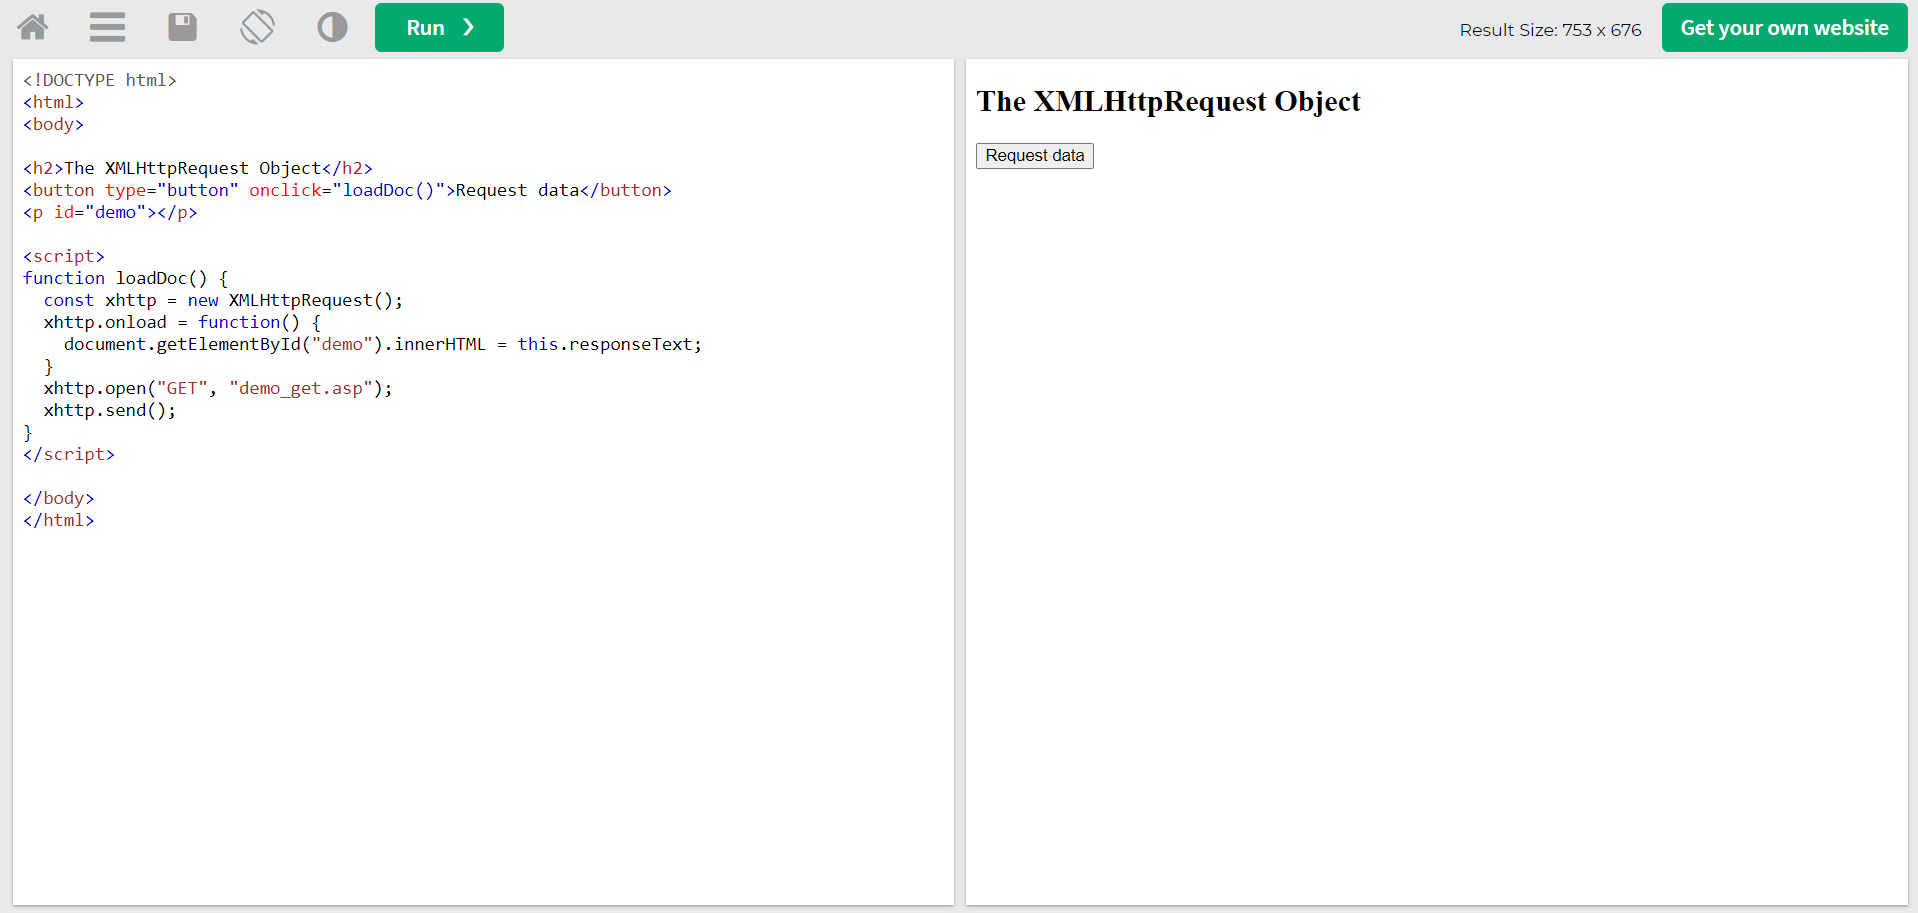
\includegraphics[width=1\textwidth,keepaspectratio]{img/ejemplo4}
				\caption{Ejemplo 1 - GET}
			\end{figure}
			\newpage
			\begin{figure}[H]
				\centering
				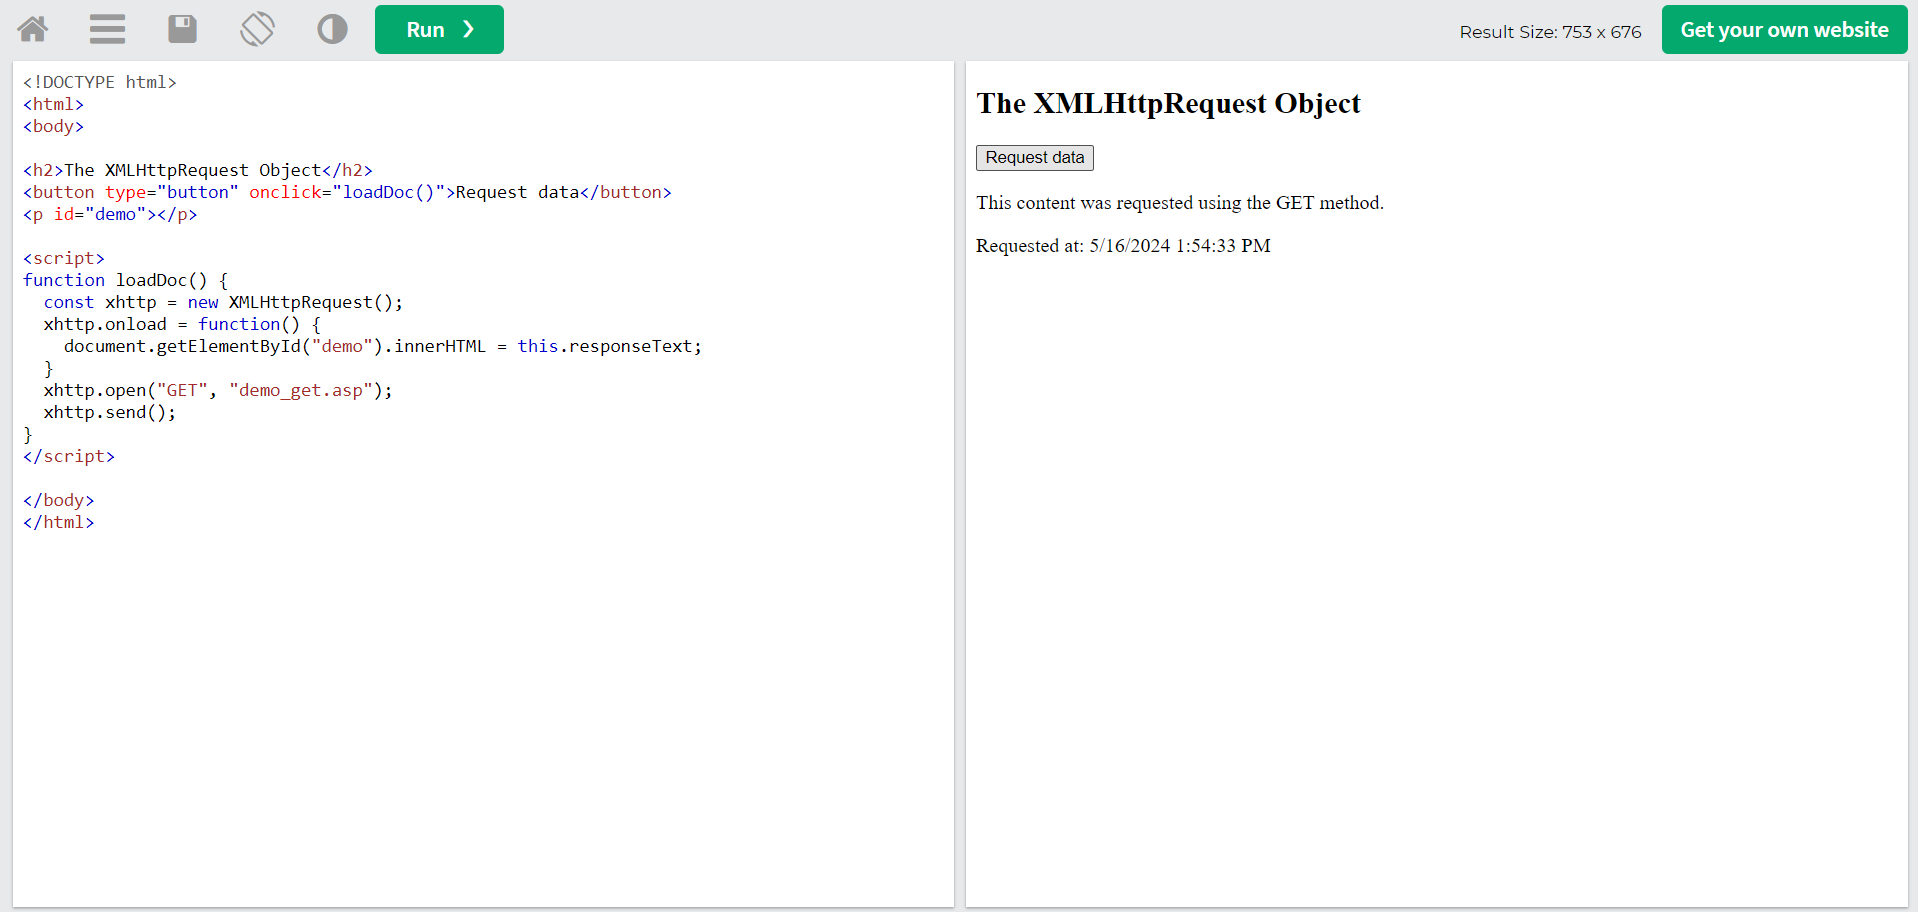
\includegraphics[width=1\textwidth,keepaspectratio]{img/boton4.png}
				\caption{Presionando botón}
			\end{figure}
			\item Segundo Ejemplo:
			\begin{figure}[H]
				\centering
				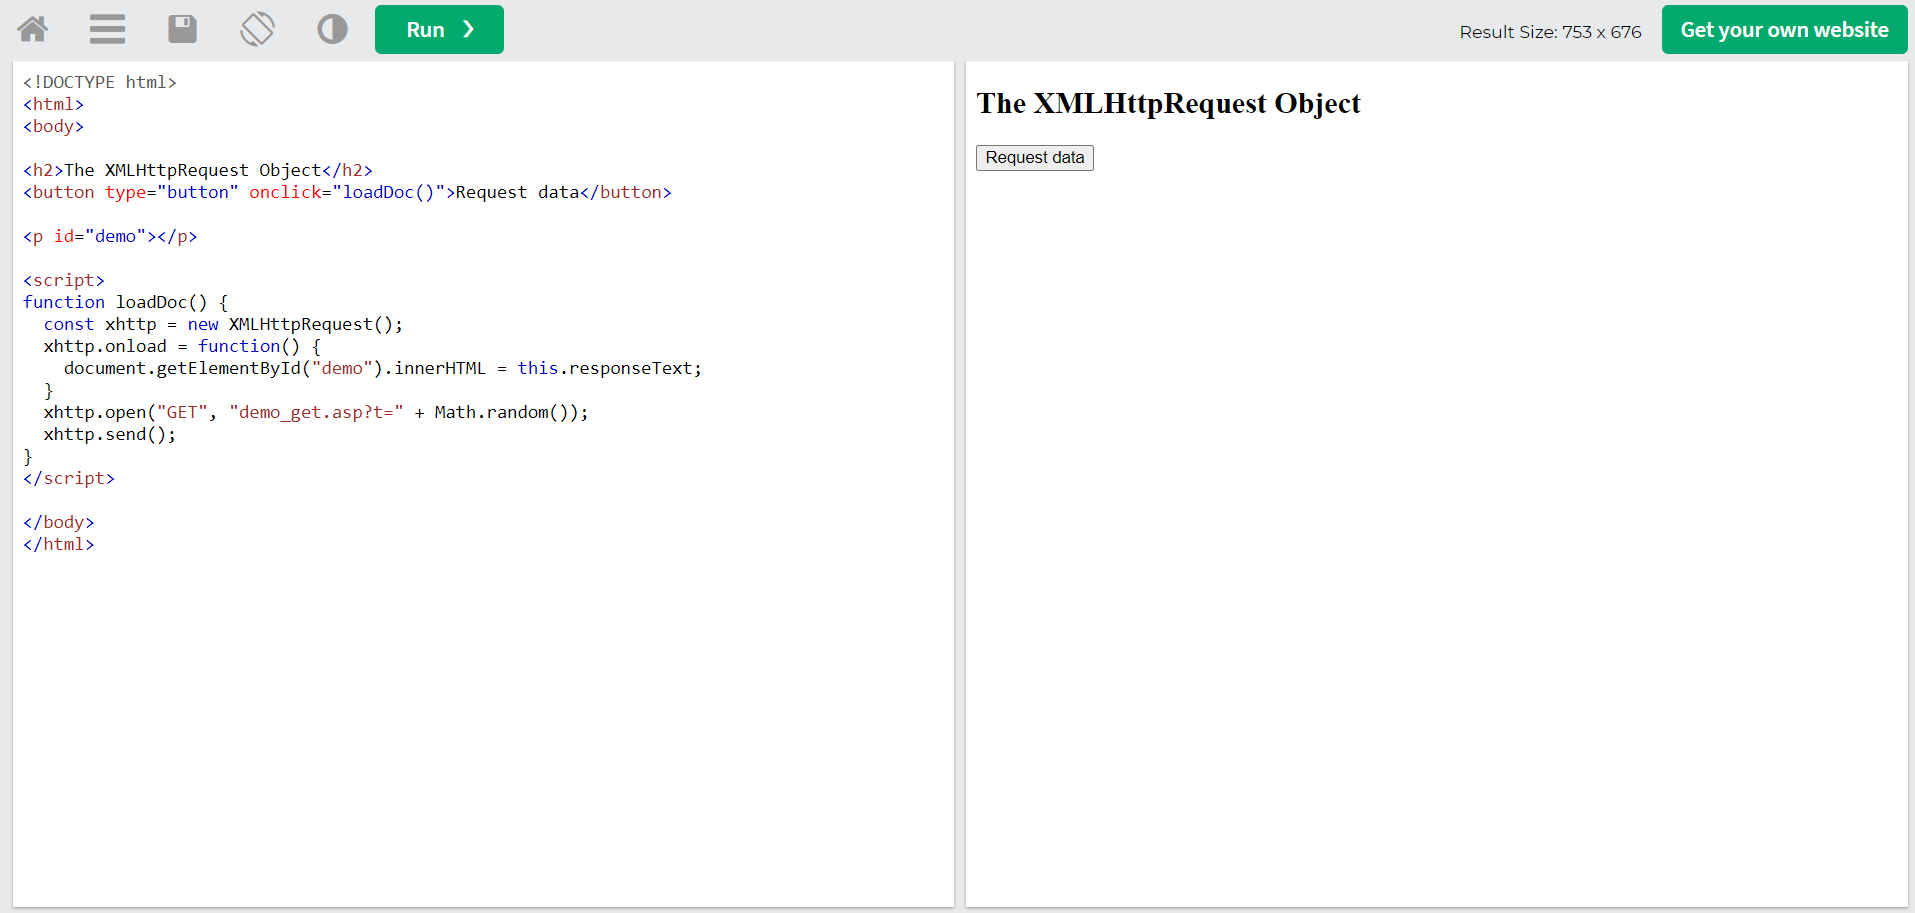
\includegraphics[width=1\textwidth,keepaspectratio]{img/ejemplo5.png}
				\caption{Ejemplo 2 - GET}
			\end{figure}
			\newpage
			\begin{figure}[H]
				\centering
				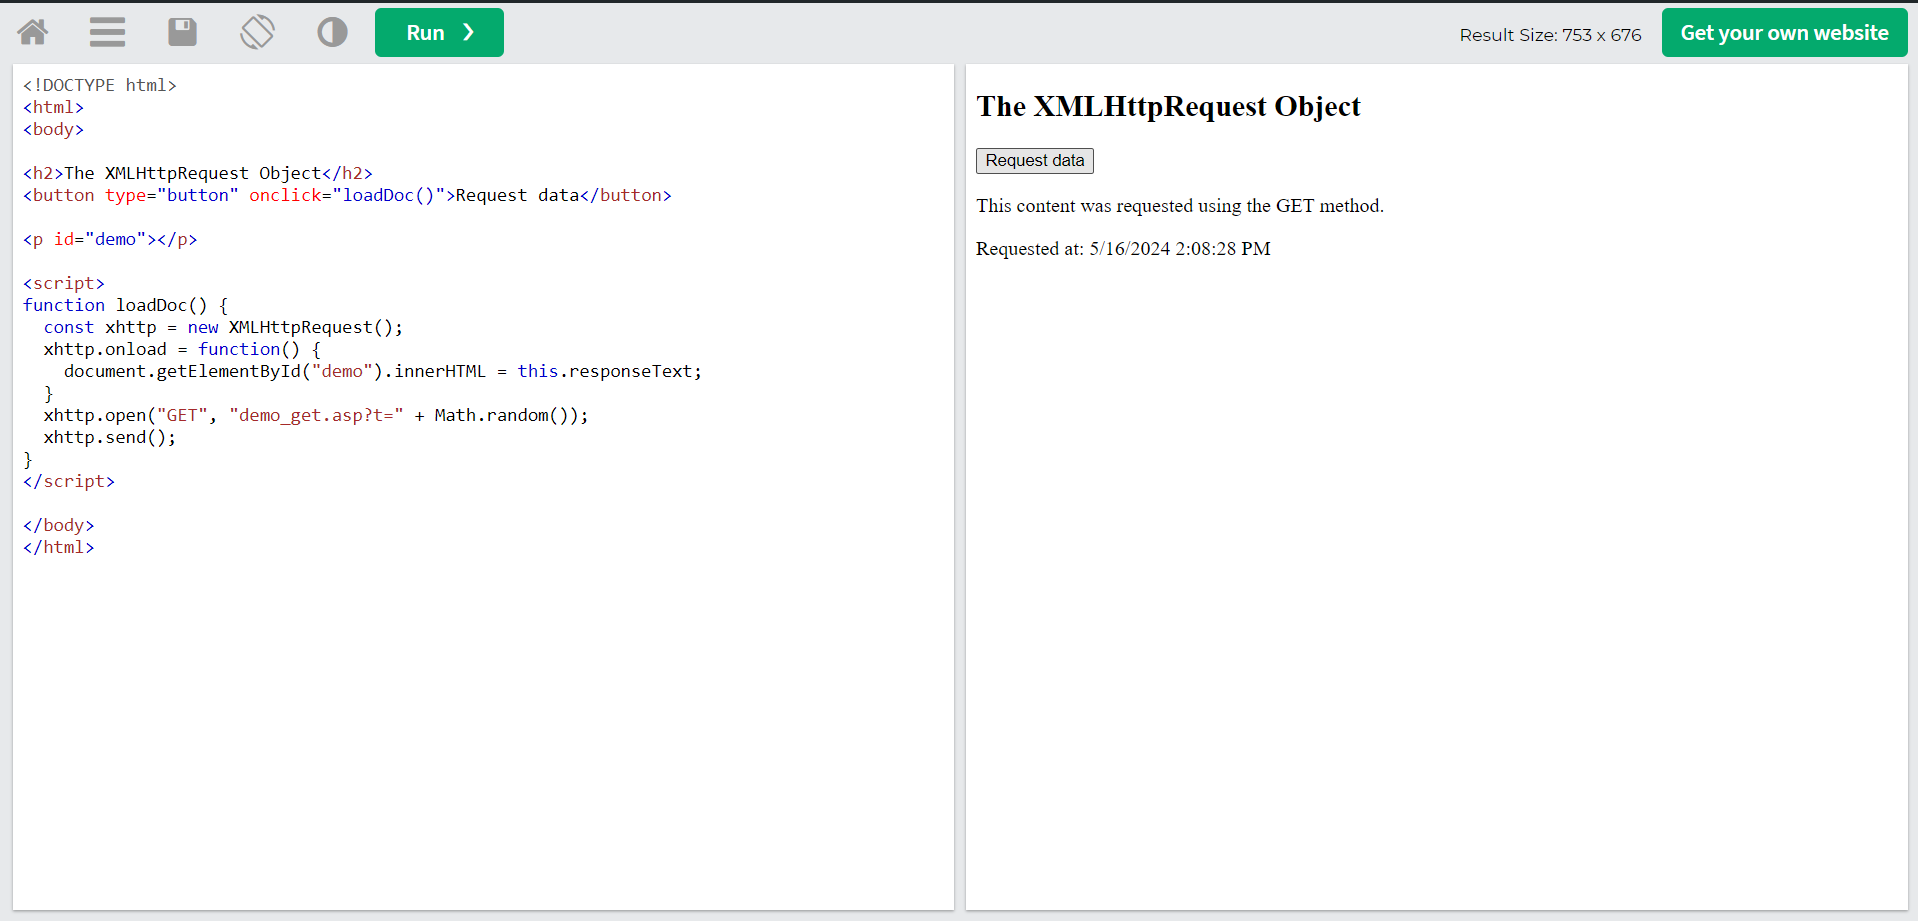
\includegraphics[width=1\textwidth,keepaspectratio]{img/boton5.png}
				\caption{Presionando el botón}
			\end{figure}
			\item Tercer Ejemplo:
			\begin{figure}[H]
				\centering
				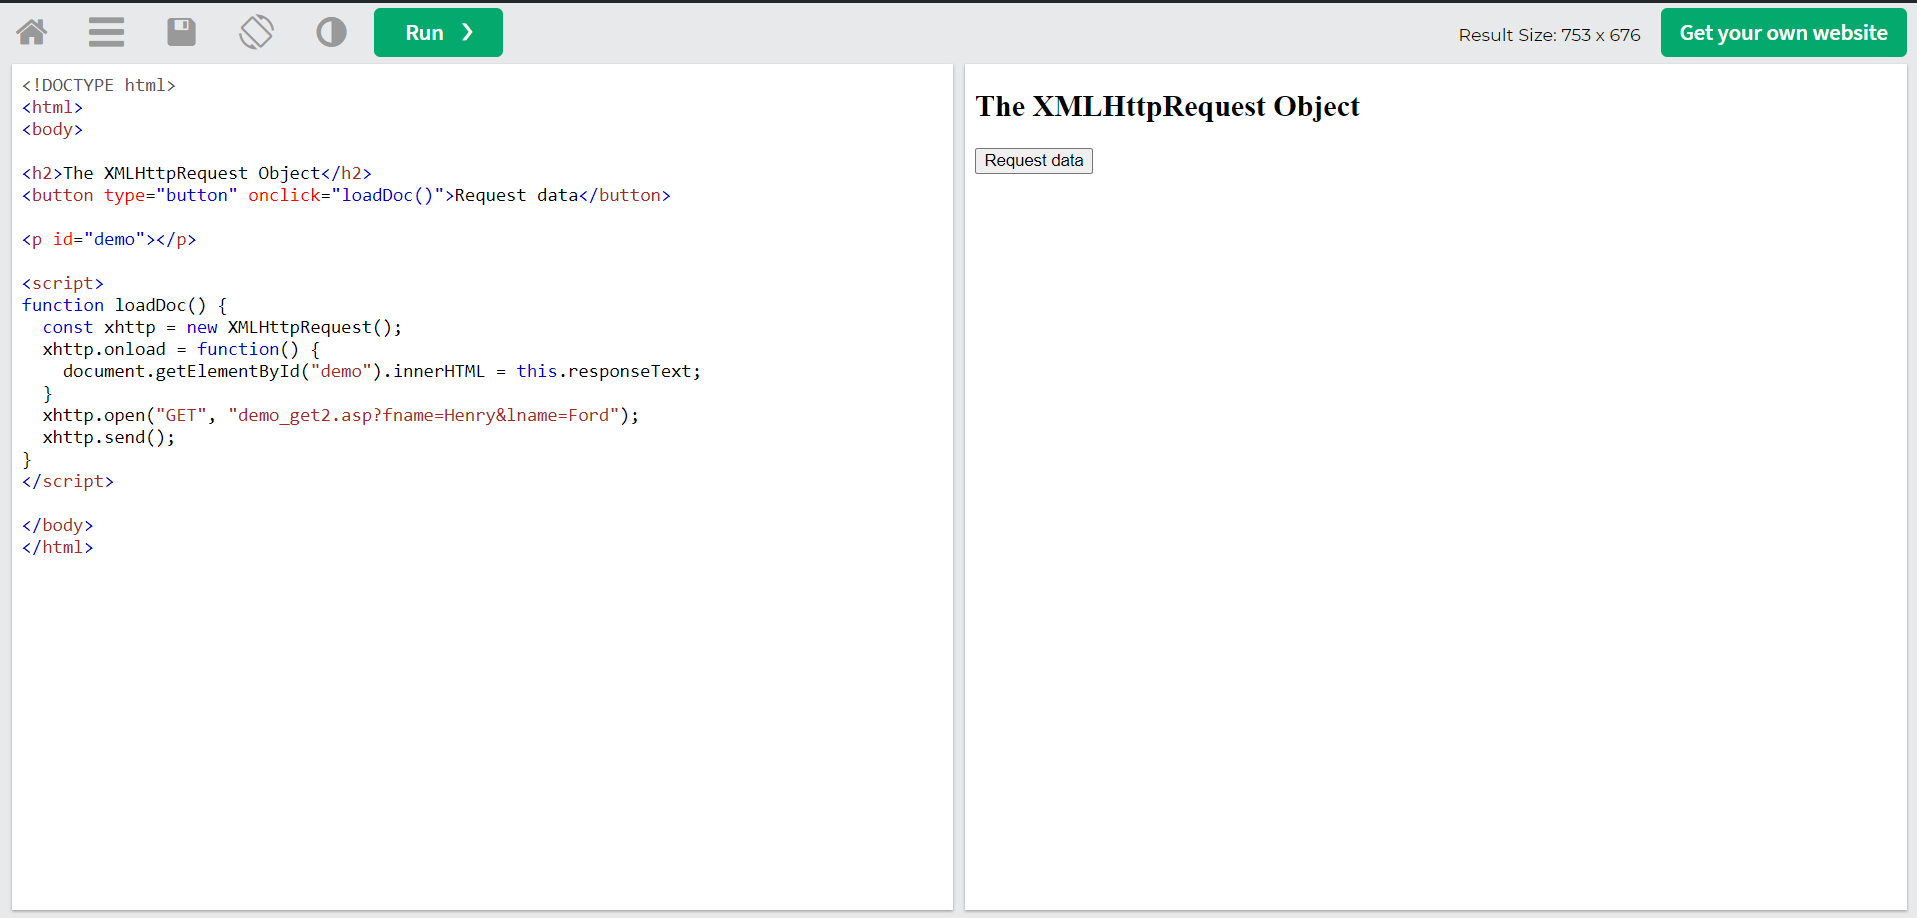
\includegraphics[width=1\textwidth,keepaspectratio]{img/ejemplo6.png}
				\caption{Ejemplo 3 - GET}
			\end{figure}
			\begin{figure}[H]
				\centering
				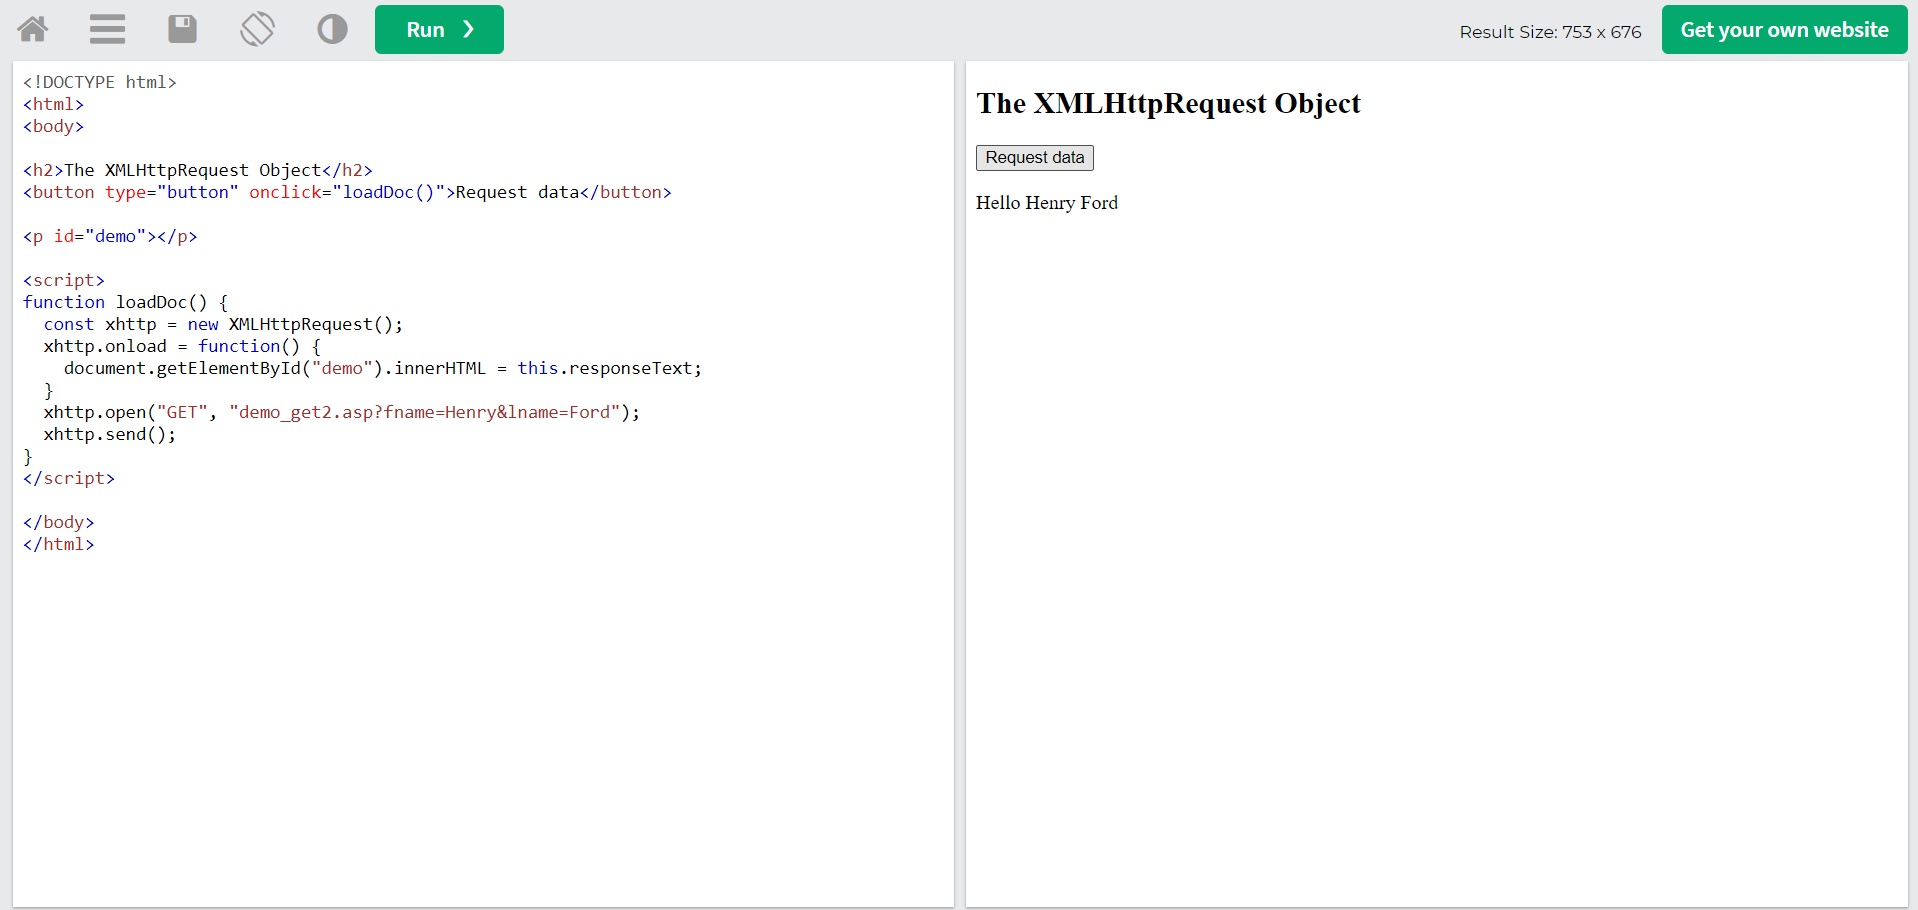
\includegraphics[width=1\textwidth,keepaspectratio]{img/boton6.png}
				\caption{Presionando el botón}
			\end{figure}
		\end{enumerate}
		\item \textbf{Post Request:}
		\begin{enumerate}
			\item Primer Ejemplo:
			\begin{figure}[H]
				\centering
				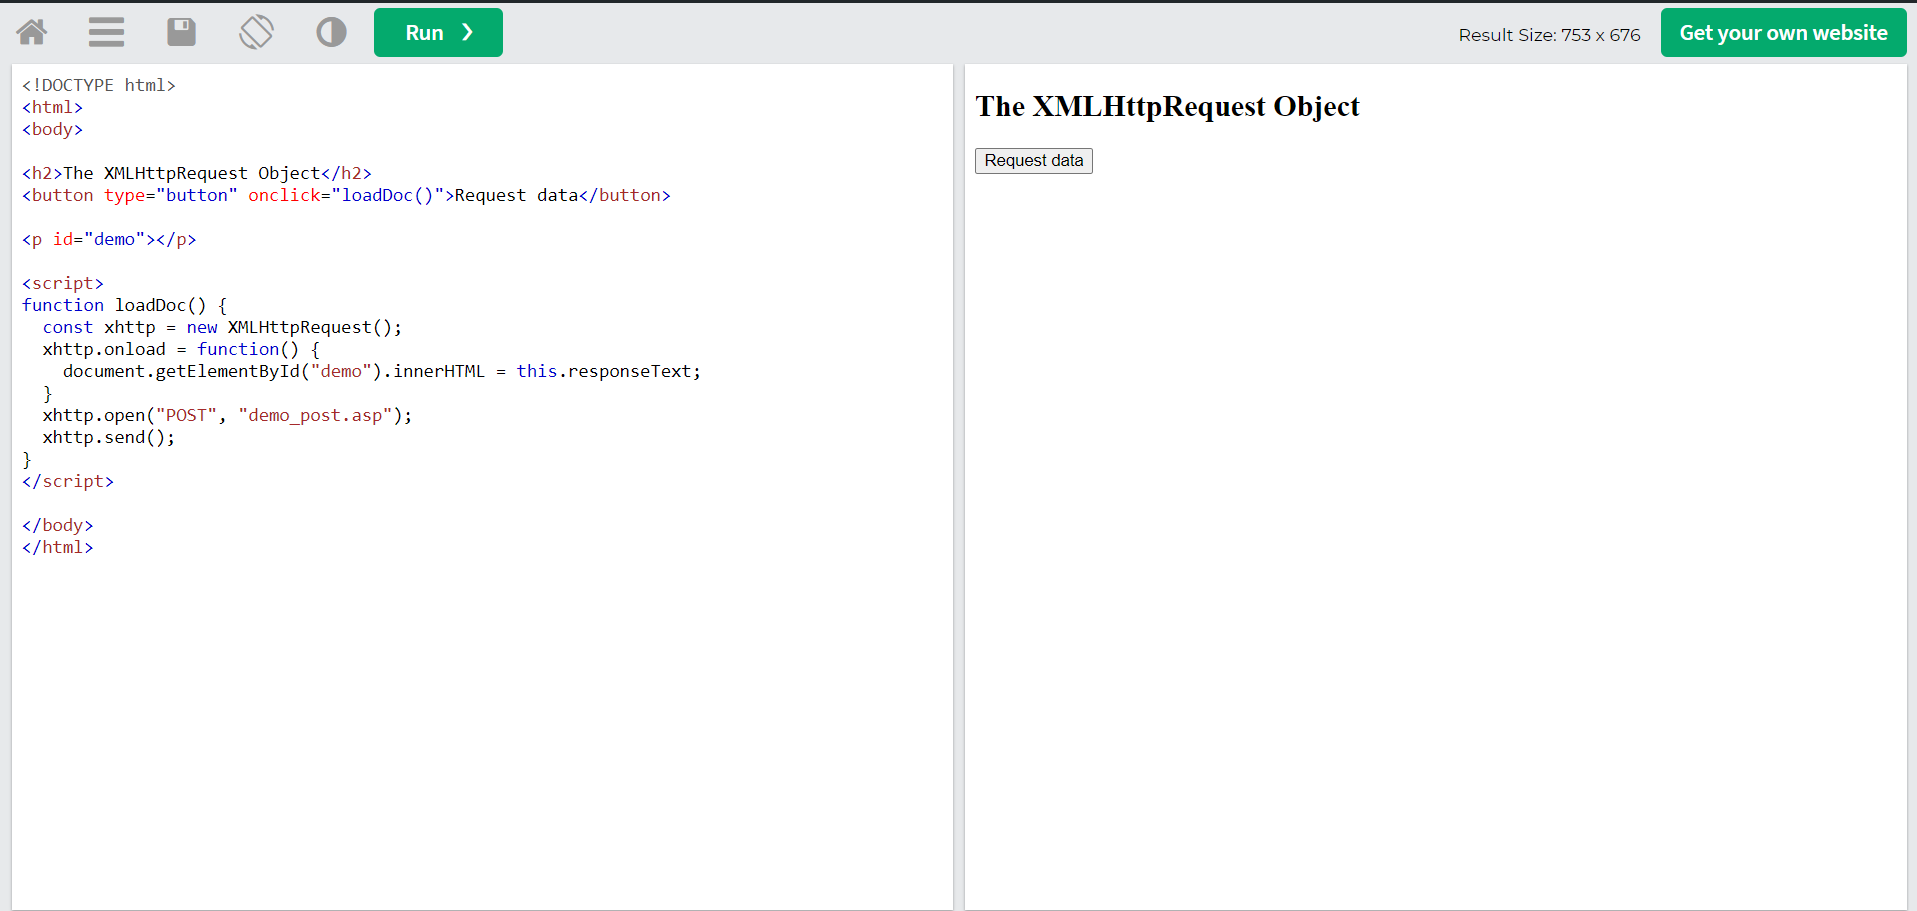
\includegraphics[width=1\textwidth,keepaspectratio]{img/ejemplo7.png}
				\caption{Ejemplo 1 - POST}
			\end{figure}
			\begin{figure}[H]
				\centering
				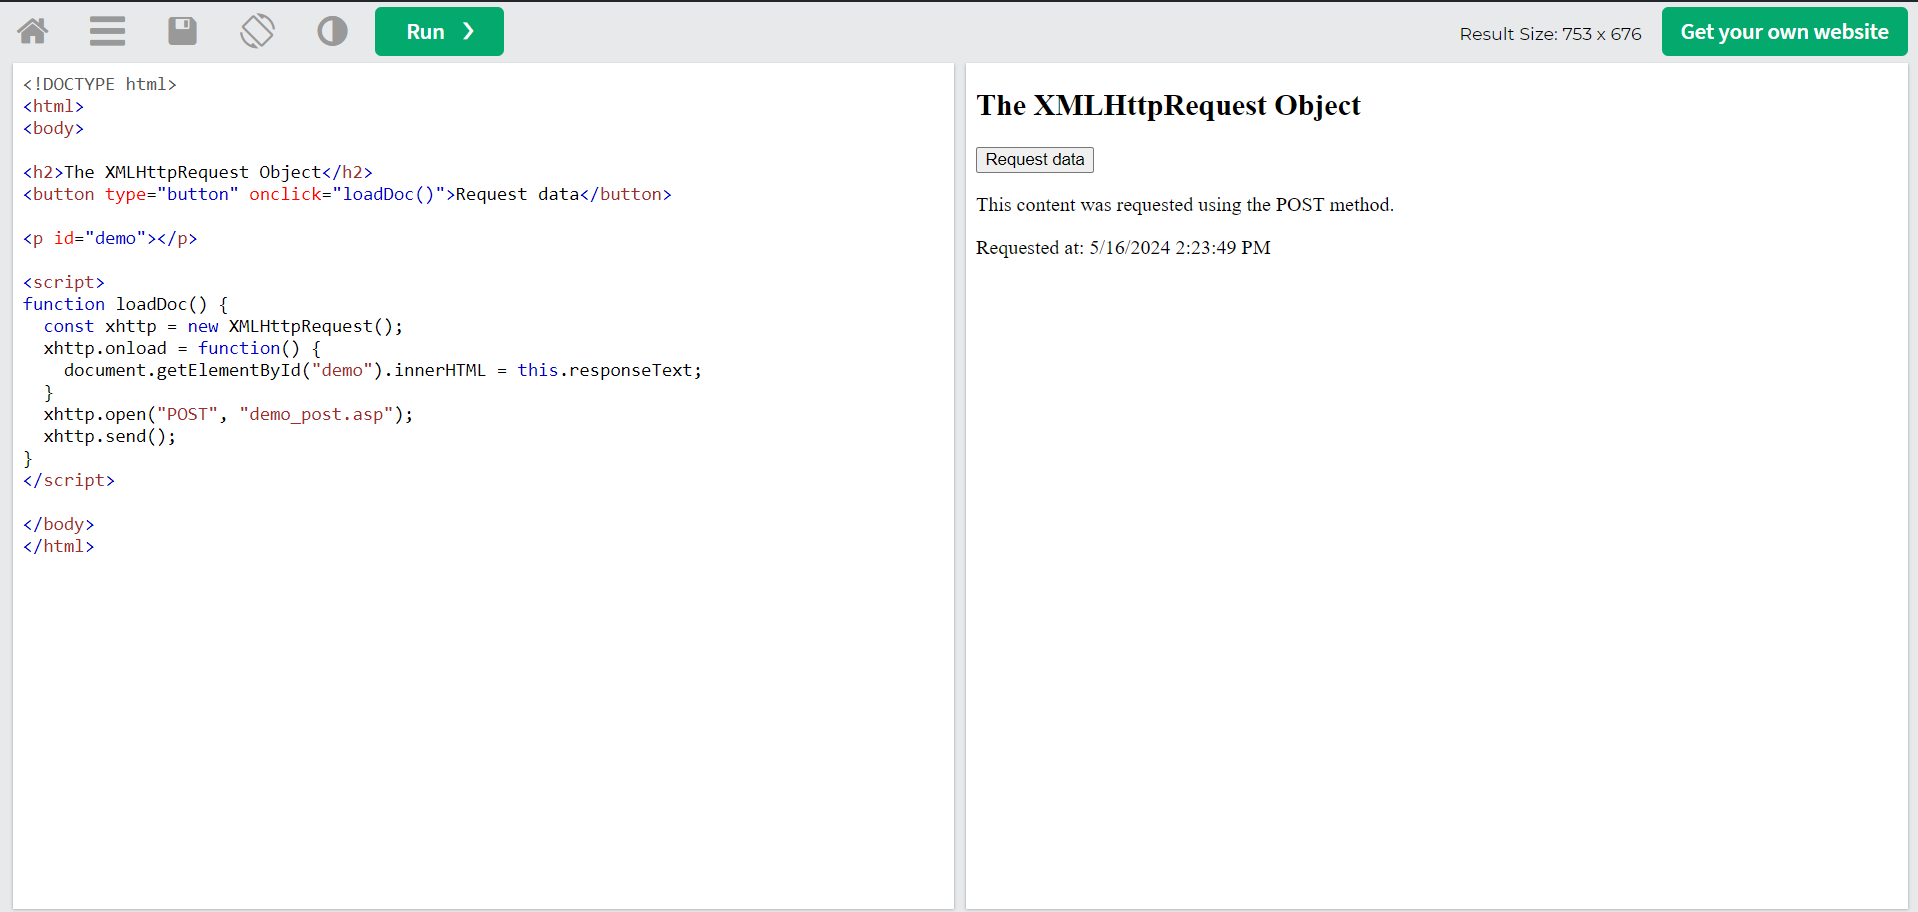
\includegraphics[width=1\textwidth,keepaspectratio]{img/boton7.png}
				\caption{Presionando el botón}
			\end{figure}
			\item Segundo Ejemplo:
			\begin{figure}[H]
				\centering
				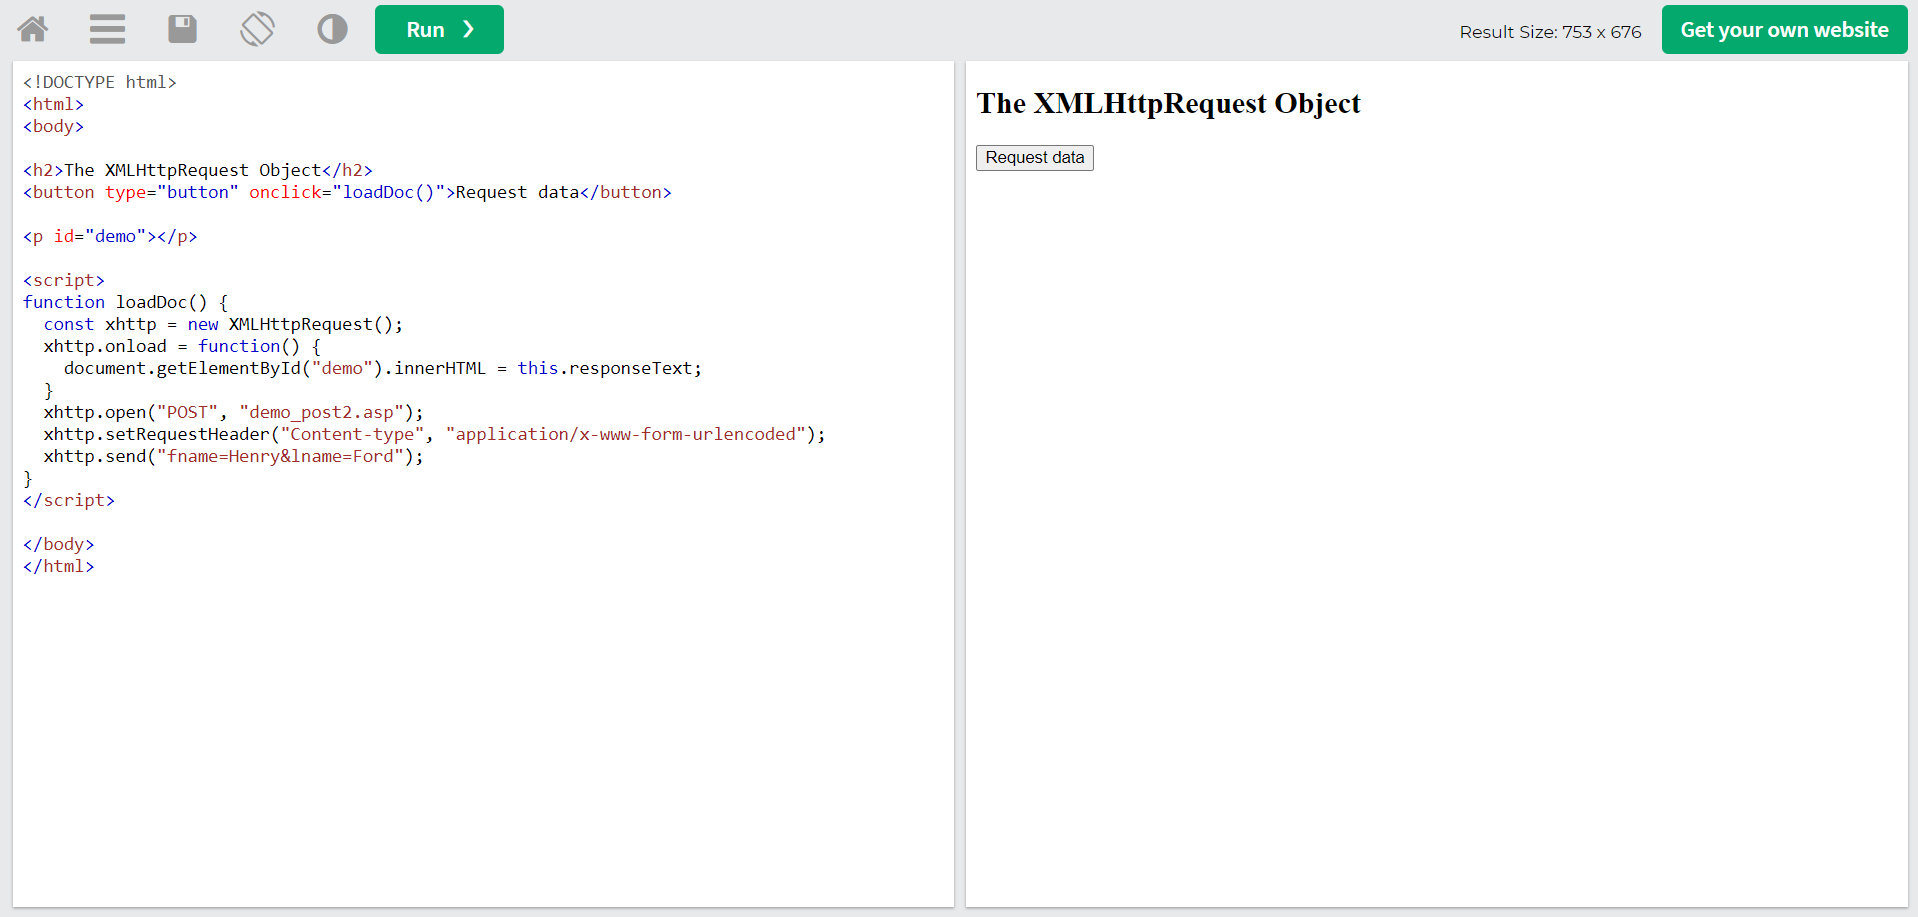
\includegraphics[width=1\textwidth,keepaspectratio]{img/ejemplo8.png}
				\caption{Ejemplo 2 - POST}
			\end{figure}
			\begin{figure}[H]
				\centering
				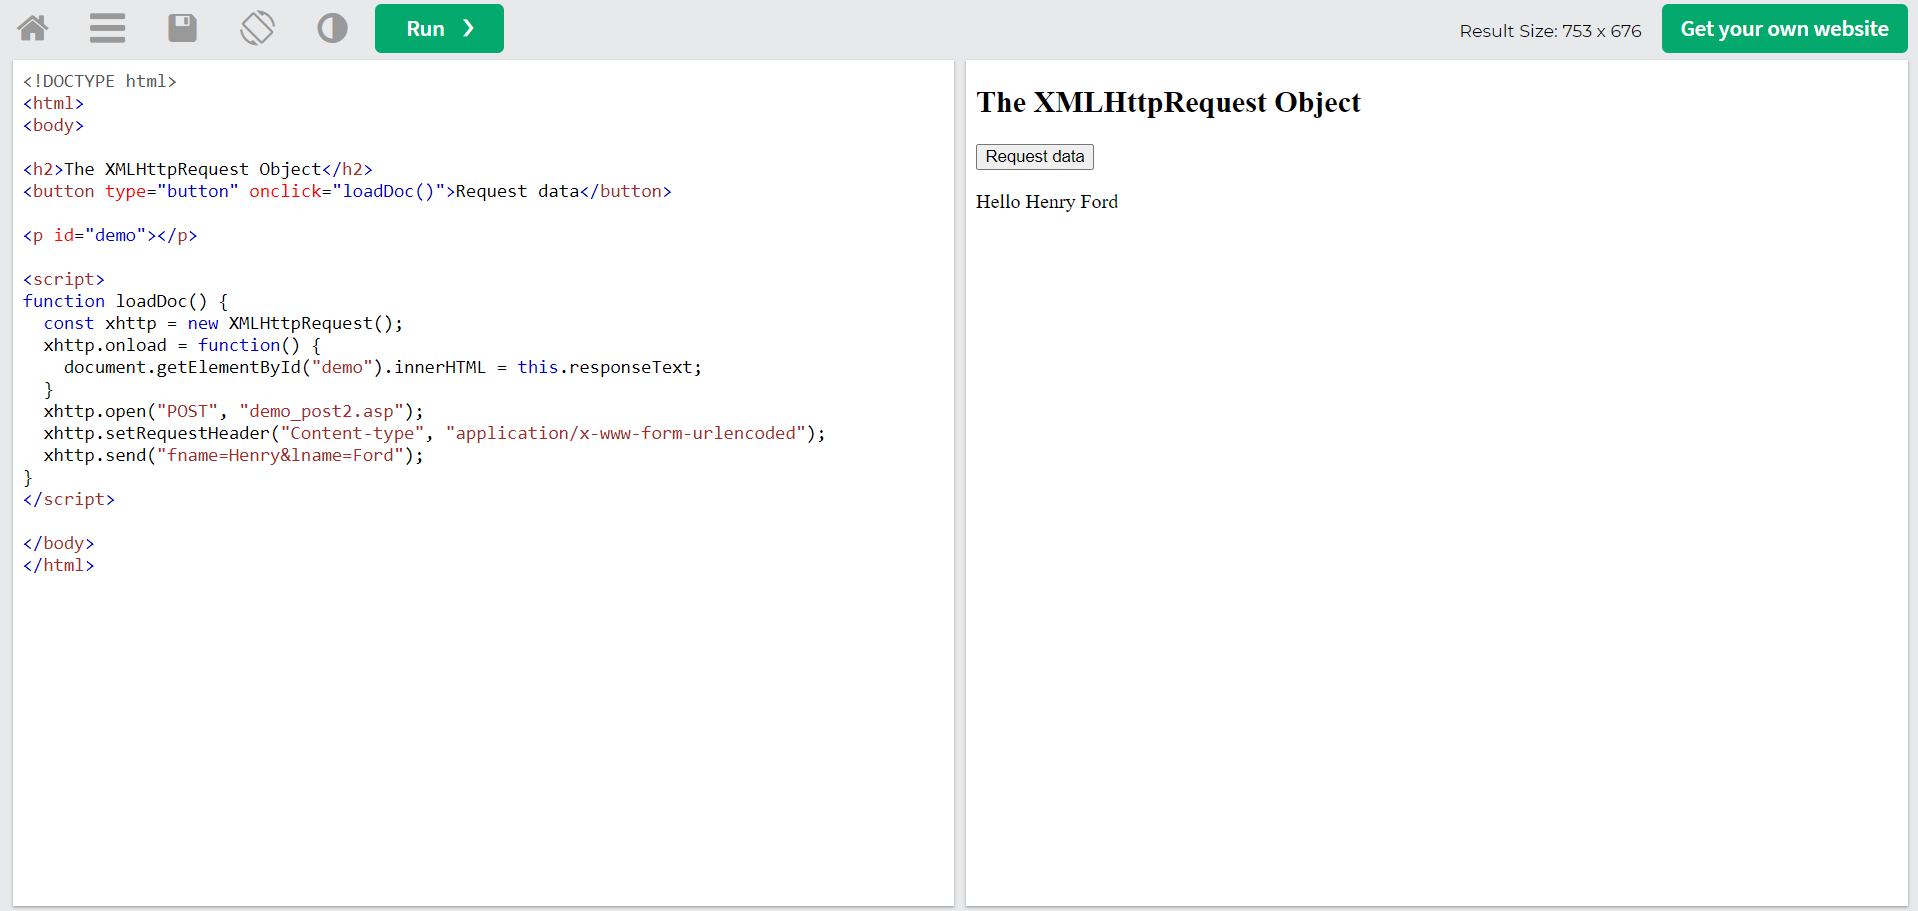
\includegraphics[width=1\textwidth,keepaspectratio]{img/boton8.png}
				\caption{Presionando el botón}
			\end{figure}
		\end{enumerate}
		\item \textbf{Synchronous Request}
		\begin{figure}[H]
			\centering
			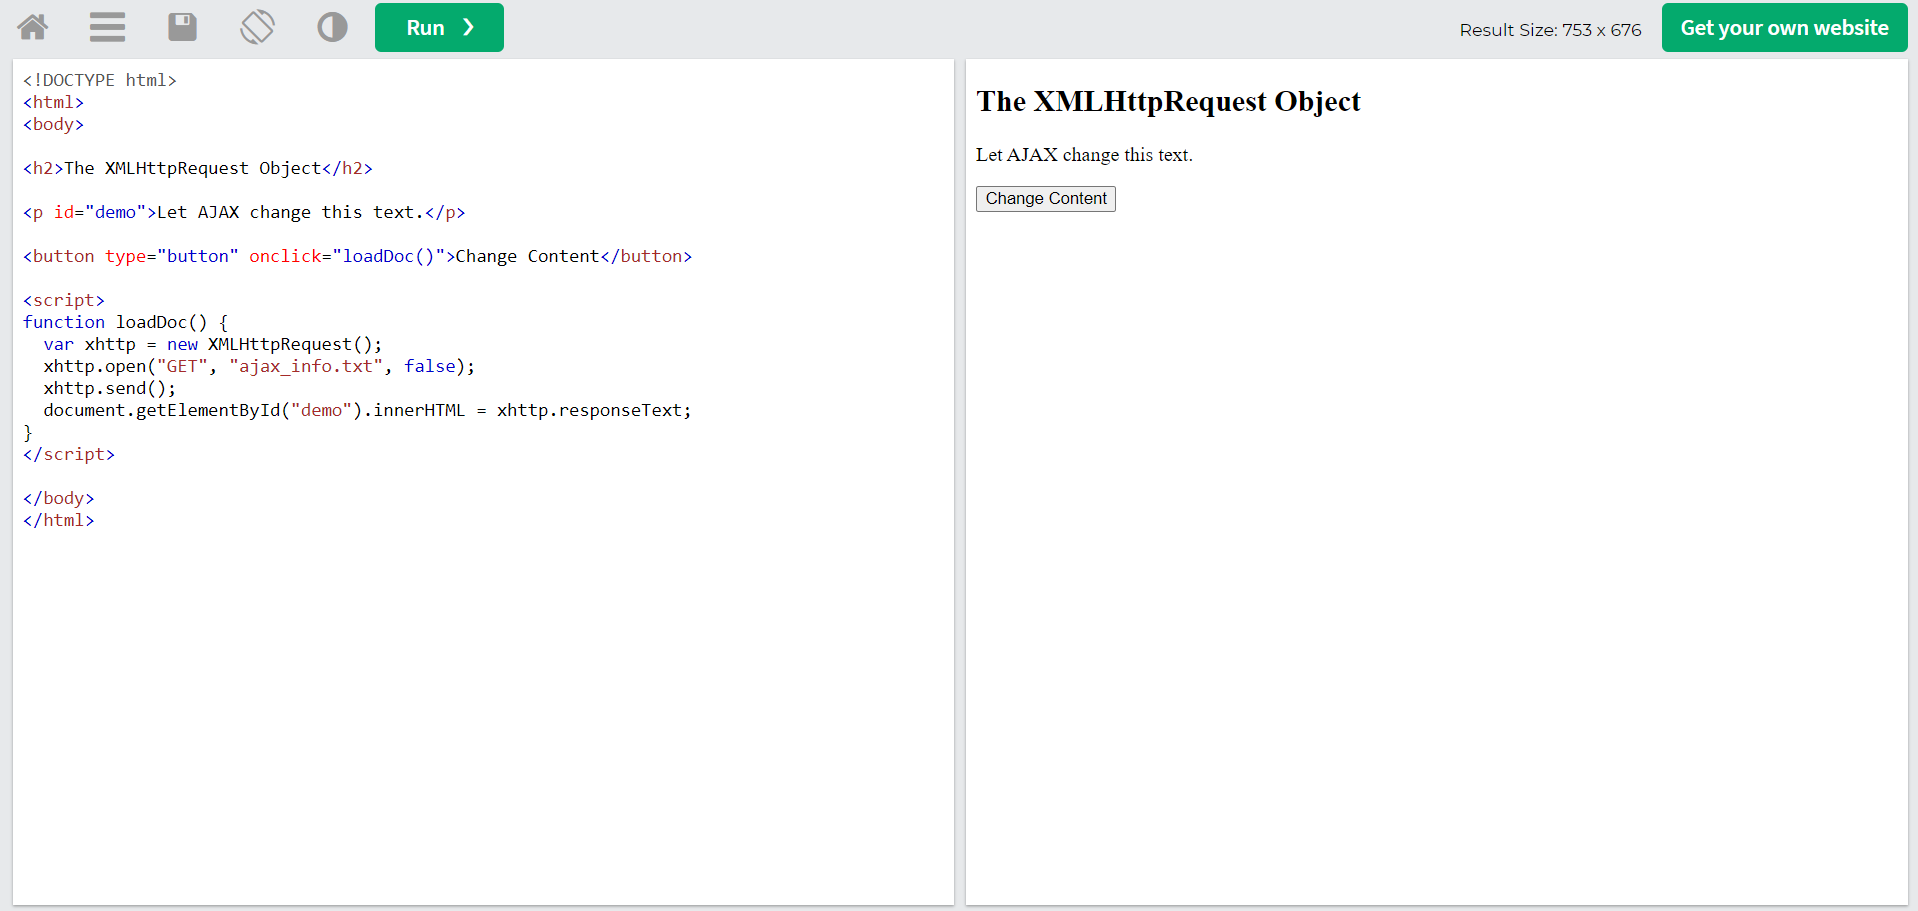
\includegraphics[width=1\textwidth,keepaspectratio]{img/ejemplo9.png}
			\caption{Ejemplo - Synchronous Request}
		\end{figure}
		\begin{figure}[H]
			\centering
			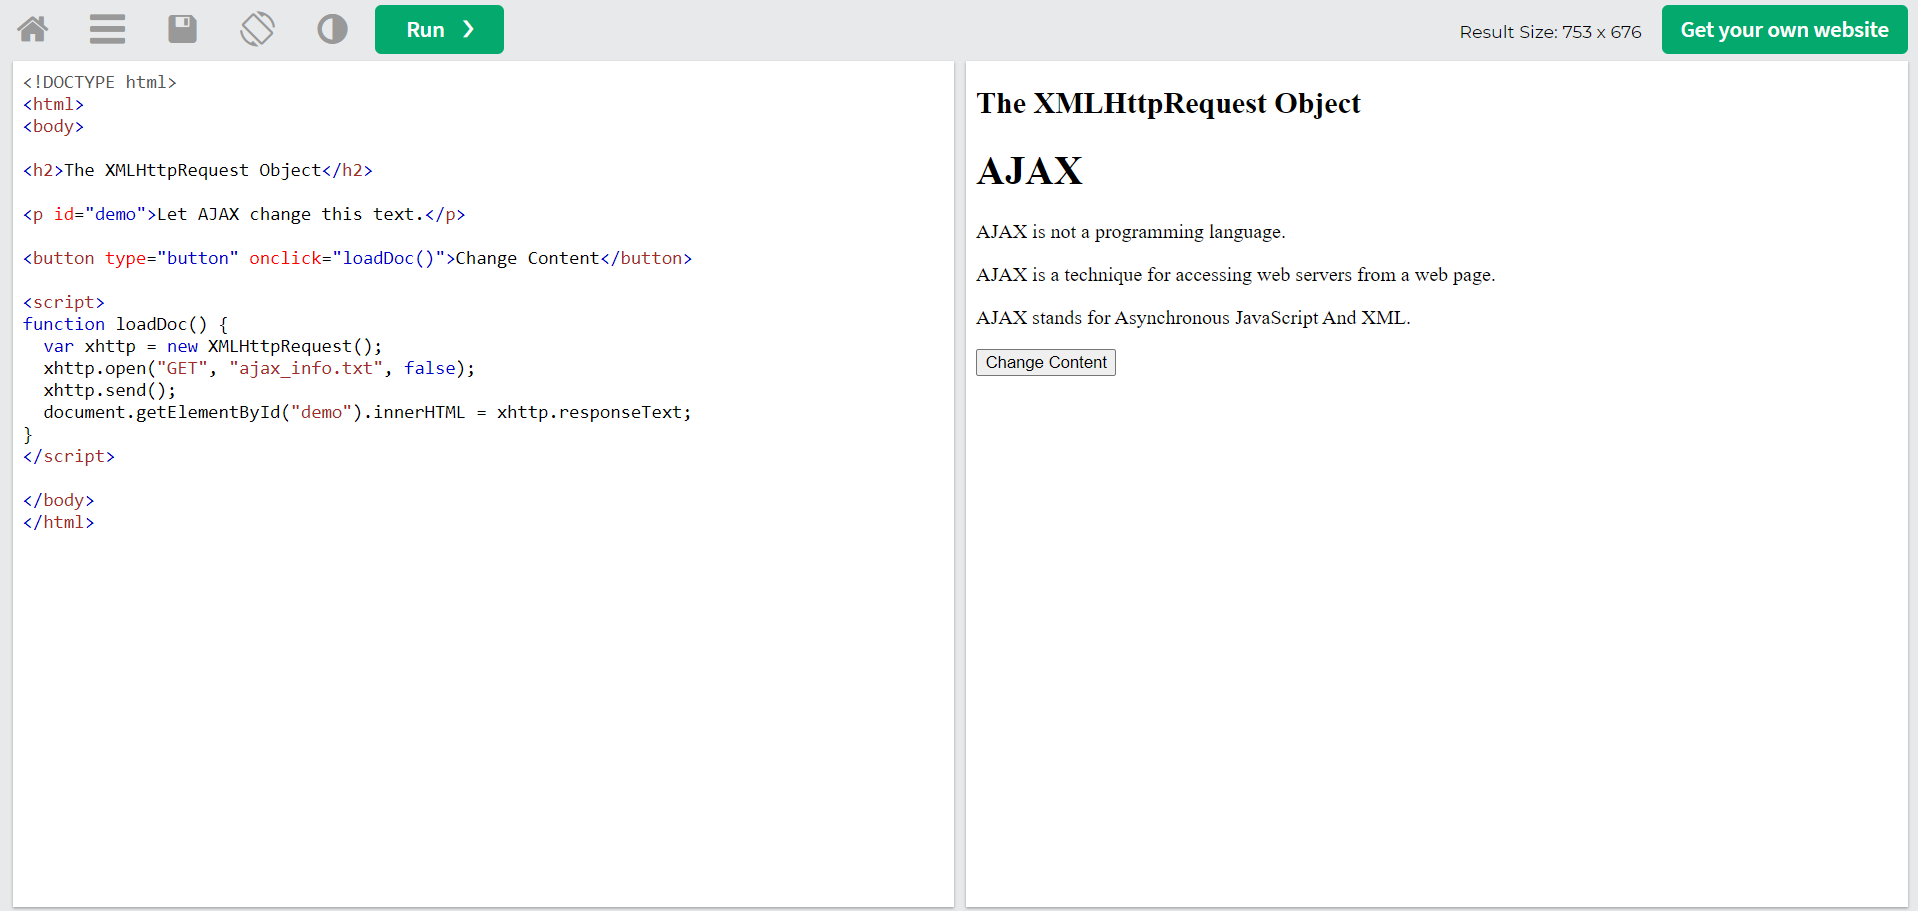
\includegraphics[width=1\textwidth,keepaspectratio]{img/boton9.png}
			\caption{Presionando el botón}
		\end{figure} 
	\end{itemize}
%%%%%%%%%%%%%%%%%%%%
	\subsubsection{AJAX - Response}
	\begin{itemize}
		\item \textbf{Propiedad de texto de respuesta}
		\begin{figure}[H]
			\centering
			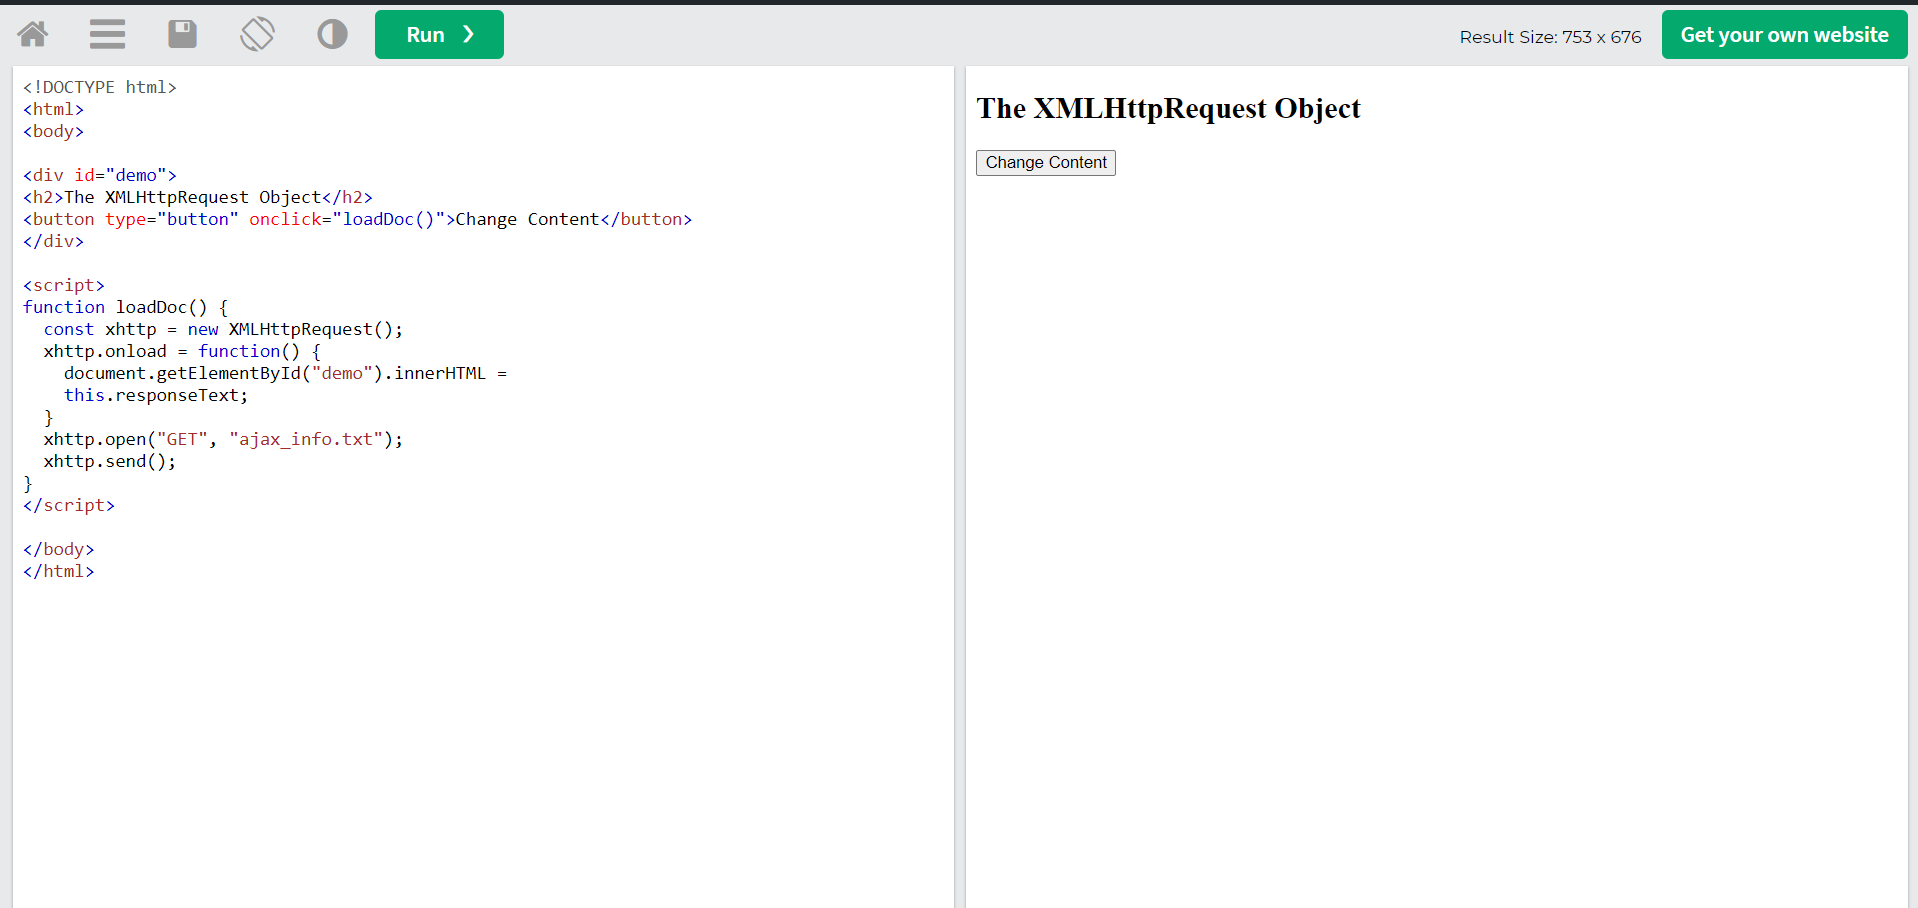
\includegraphics[width=1\textwidth,keepaspectratio]{img/ejemplo10.png}
			\caption{Propiedad de Texto de Respuesta}
		\end{figure}
		\begin{figure}[H]
			\centering
			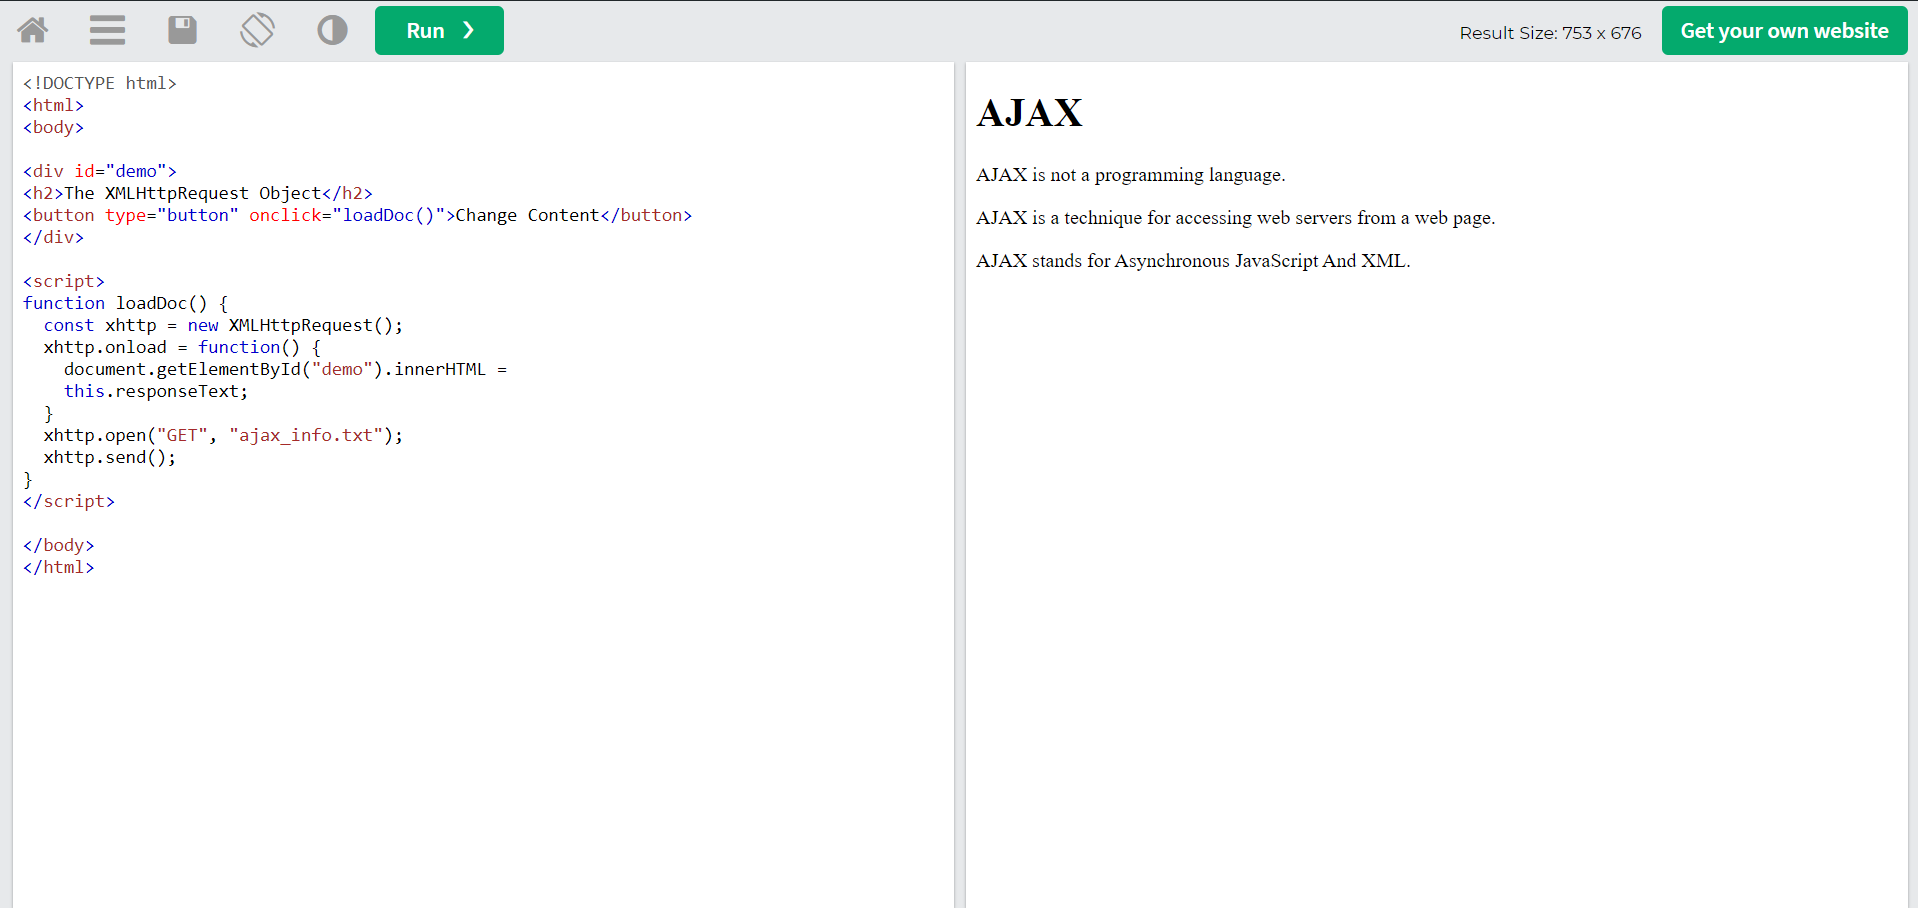
\includegraphics[width=1\textwidth,keepaspectratio]{img/boton10.png}
			\caption{Presionando el botón}
		\end{figure}
		\item \textbf{La propiedad ResponseXML}
		\begin{figure}[H]
			\centering
			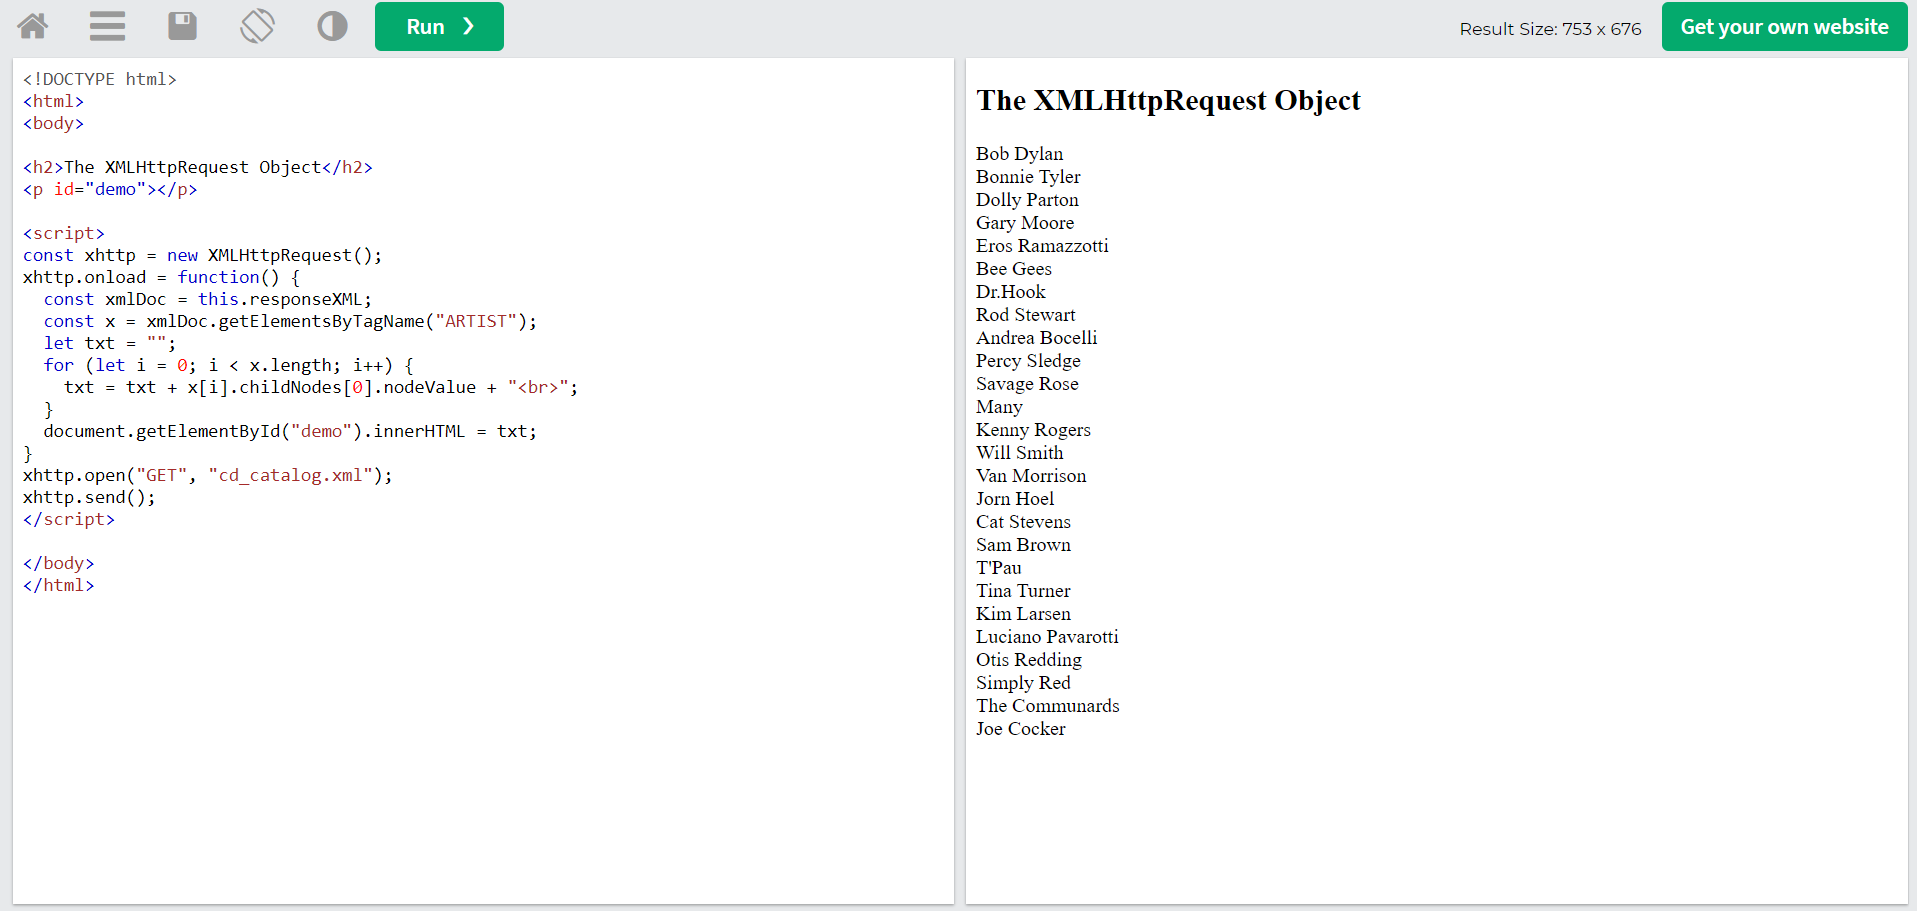
\includegraphics[width=1\textwidth,keepaspectratio]{img/ejemplo11.png}
			\caption{Propiedad de Texto de Respuesta}
		\end{figure}
		\newpage
		\item \textbf{Método getAllResponseHeaders()}
		\begin{figure}[H]
			\centering
			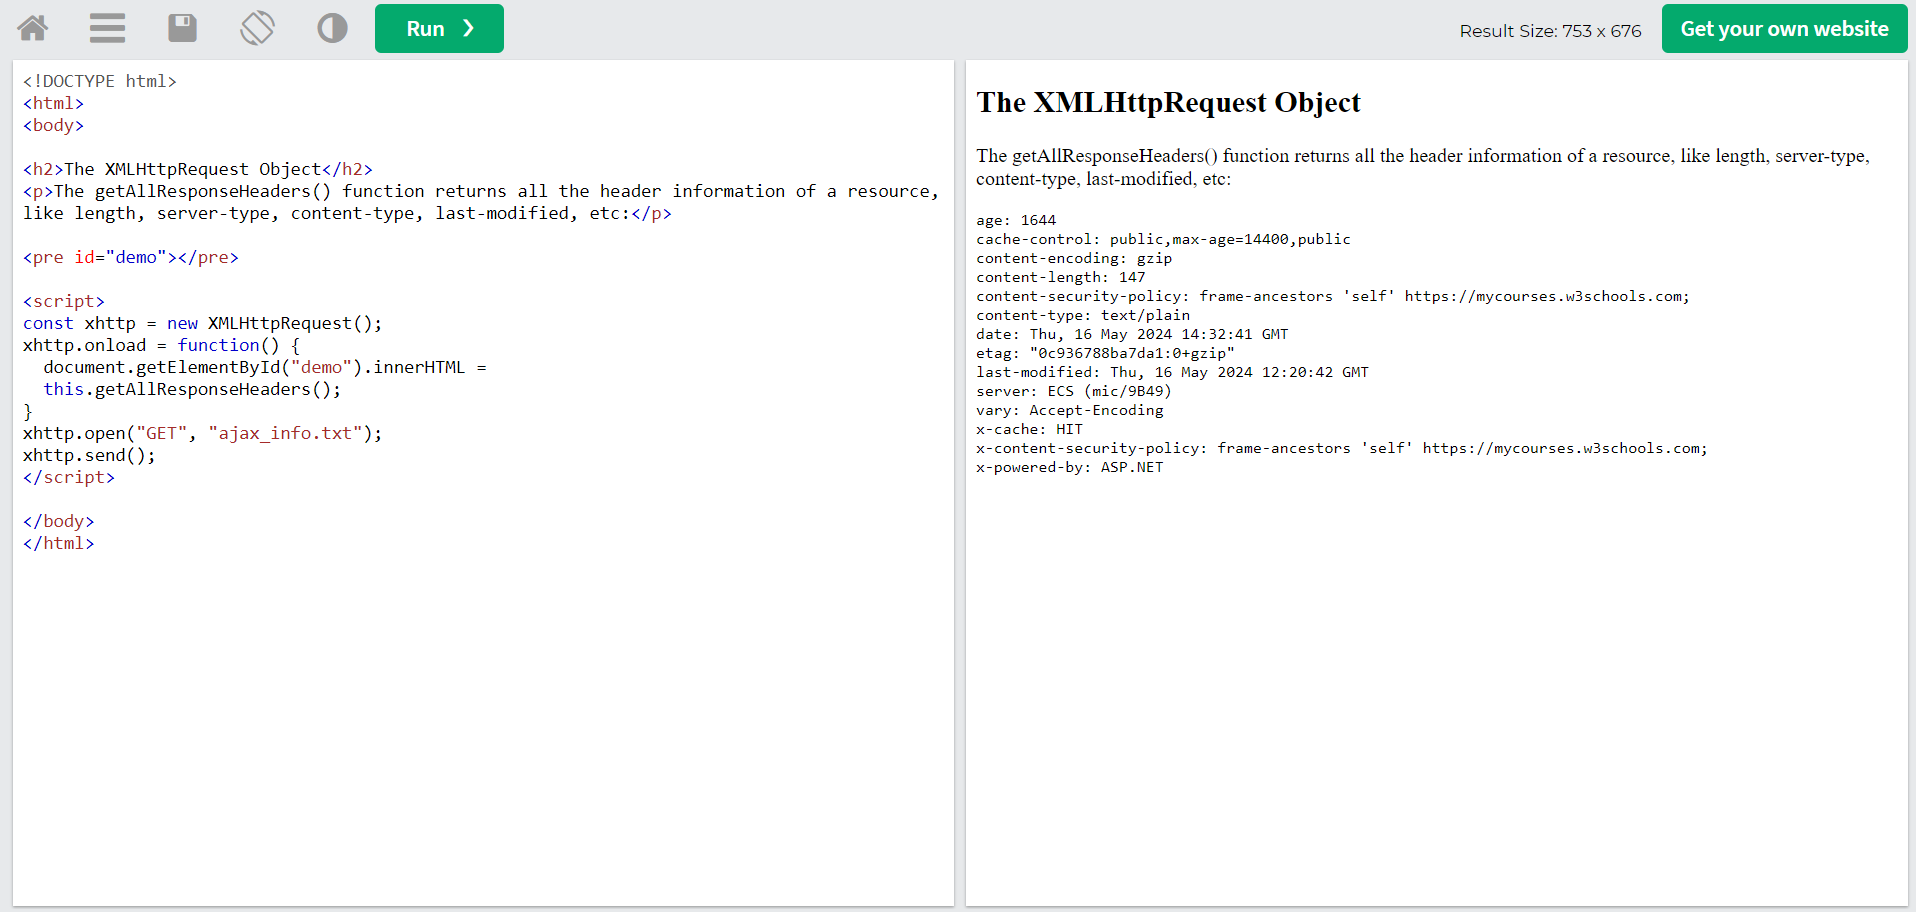
\includegraphics[width=1\textwidth,keepaspectratio]{img/ejemplo12.png}
			\caption{Método getAllResponseHeaders}
		\end{figure}
		\item \textbf{Método getResponseHeader()}
		\begin{figure}[H]
			\centering
			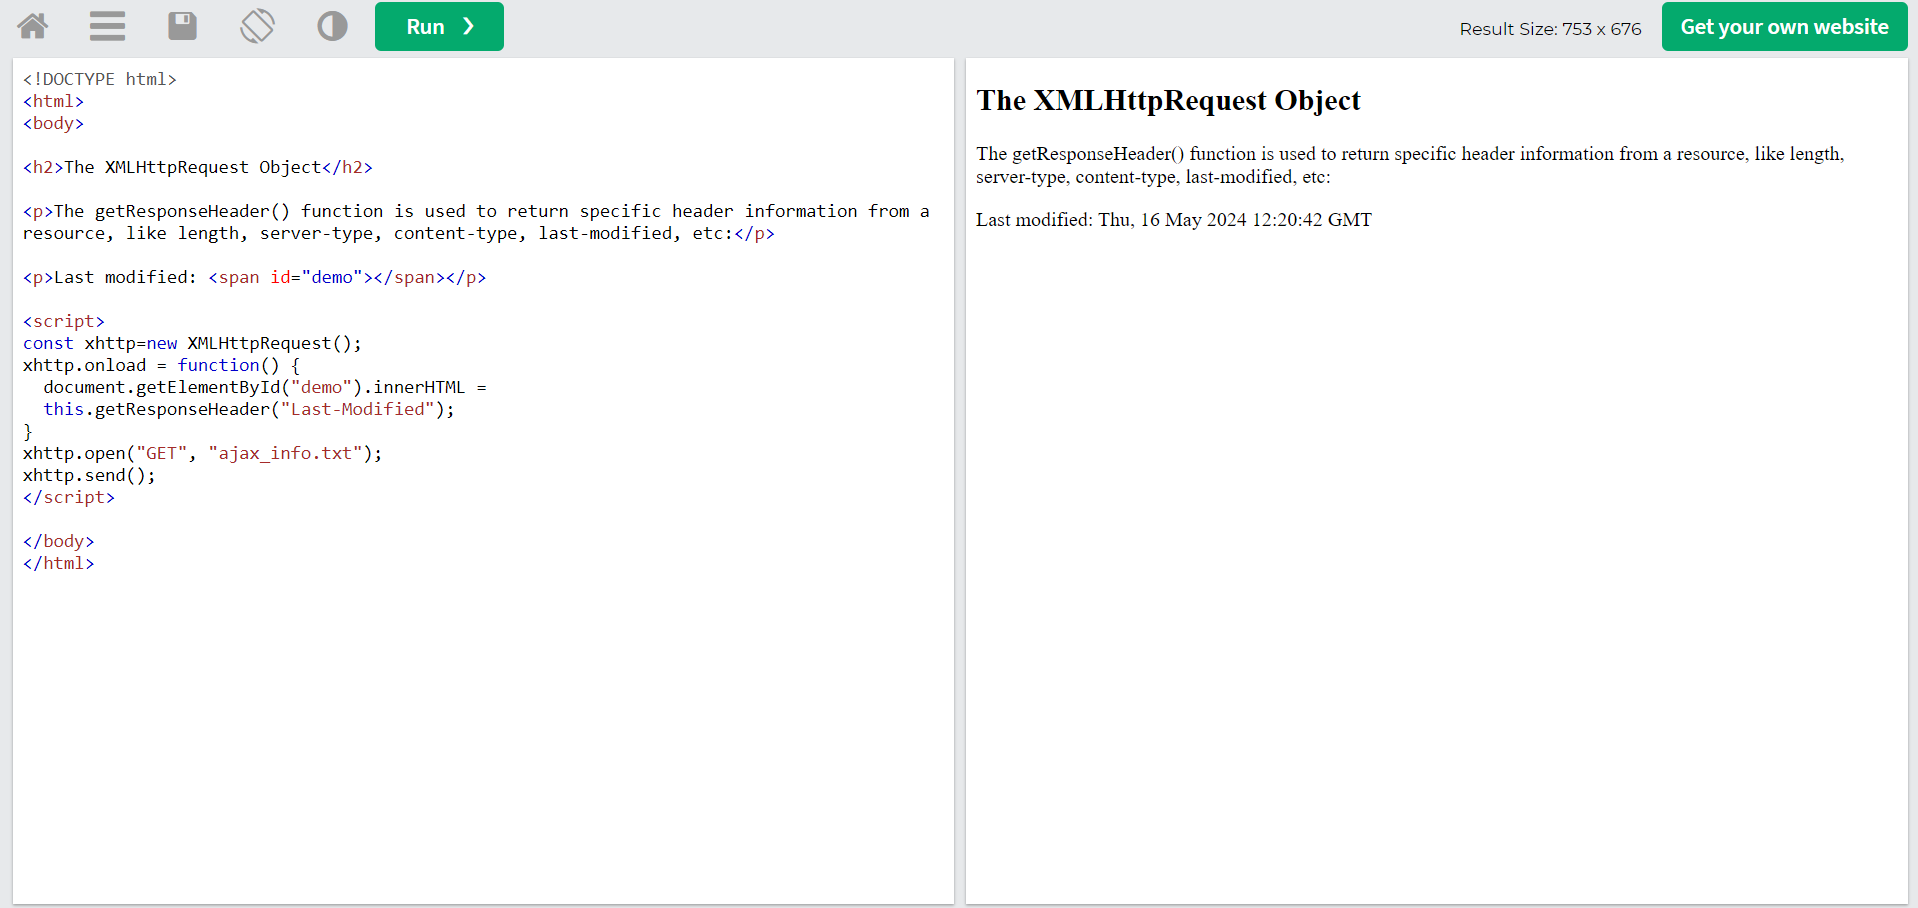
\includegraphics[width=1\textwidth,keepaspectratio]{img/ejemplo13.png}
			\caption{Método getResponseHeader}
		\end{figure}
	\end{itemize}
	\newpage
%%%%%%%%%%%%%%%%%%%%
	\subsubsection{AJAX XML - File}
	\begin{itemize}
		\item \textbf{AJAX XML EXAMPLE}
		\begin{figure}[H]
			\centering
			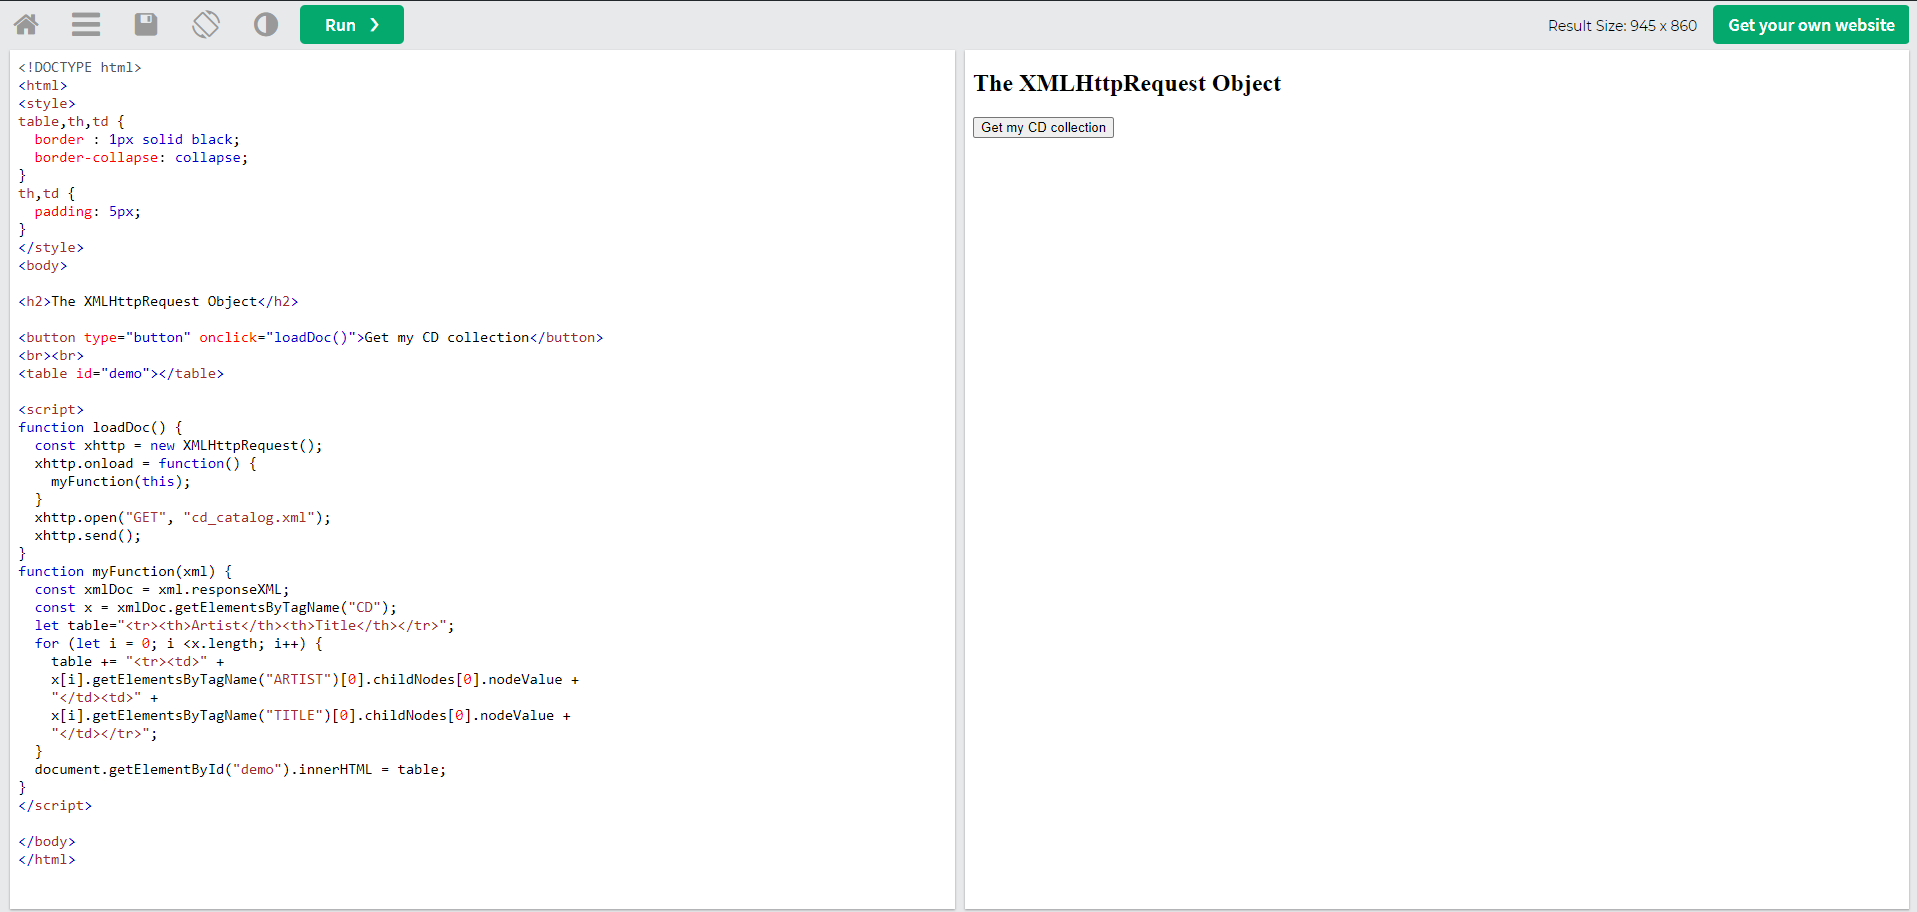
\includegraphics[width=1\textwidth,keepaspectratio]{img/ejemplo14.png}
			\caption{Ajax XML}
		\end{figure}
		\begin{figure}[H]
			\centering
			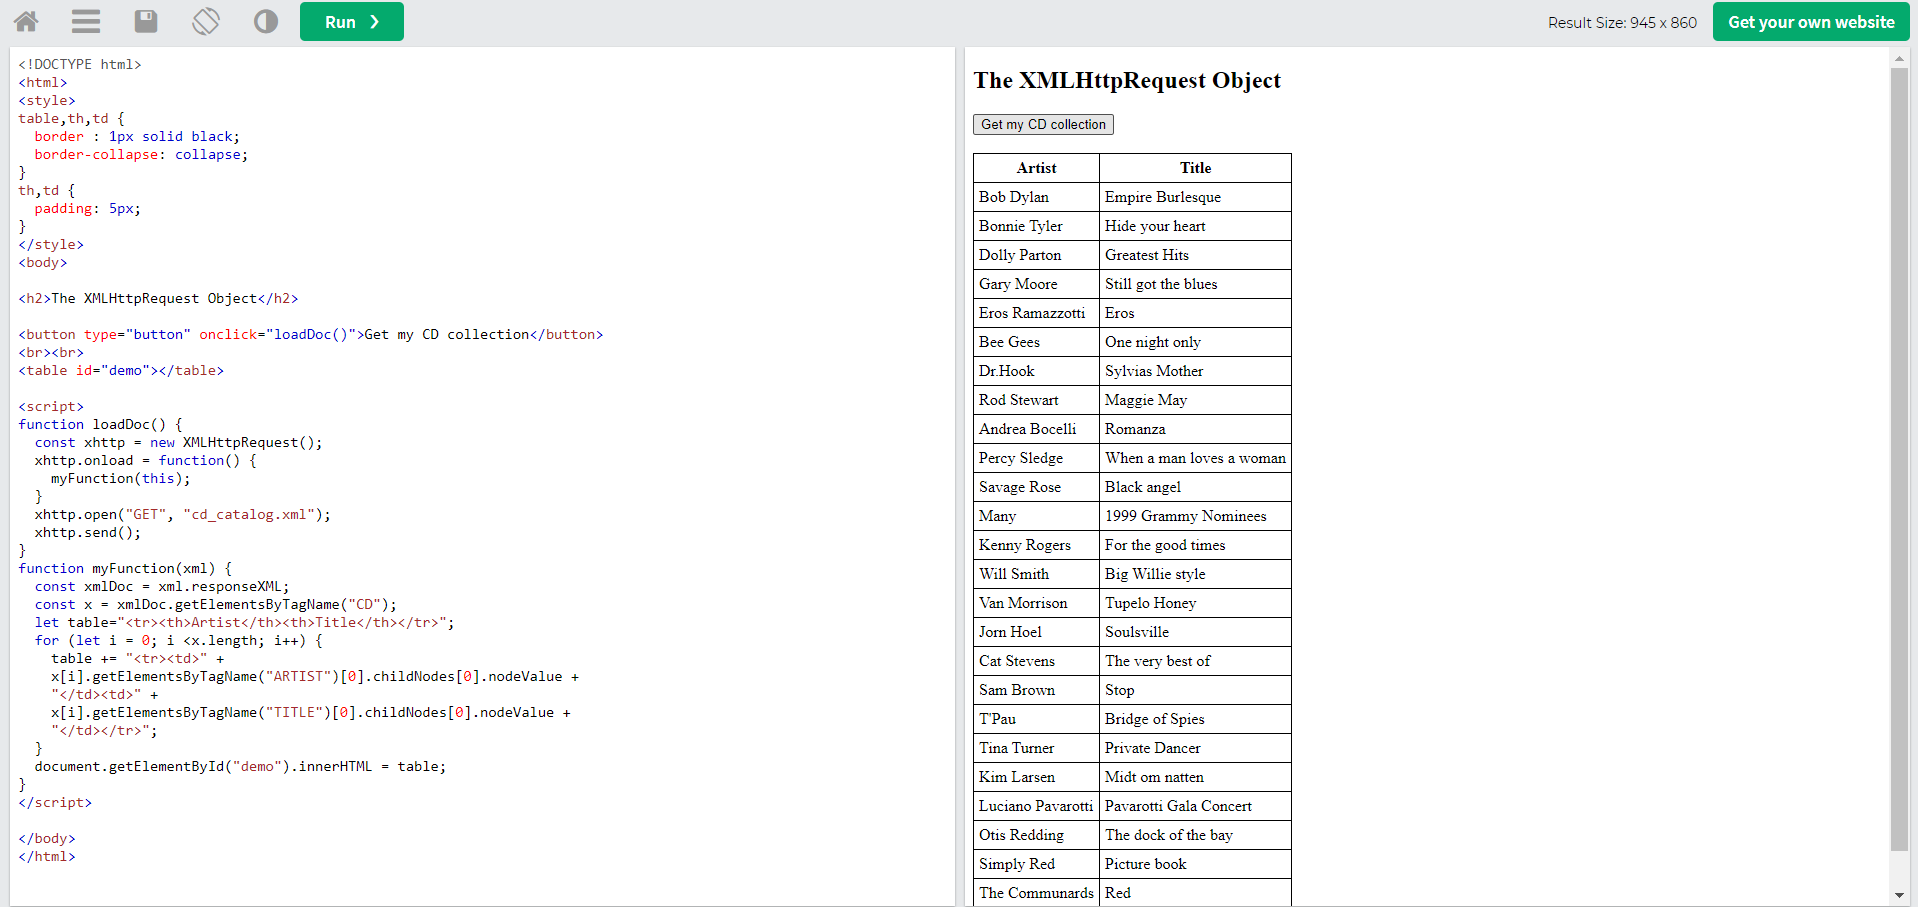
\includegraphics[width=1\textwidth,keepaspectratio]{img/boton14.png}
			\caption{Presionando el botón}
		\end{figure}
	\end{itemize}
	\newpage
%%%%%%%%%%%%%%%%%%%%
	\subsubsection{AJAX PHP}
	\begin{itemize}
		\item \textbf{AJAX PHP EXAMPLE}
		\begin{figure}[H]
			\centering
			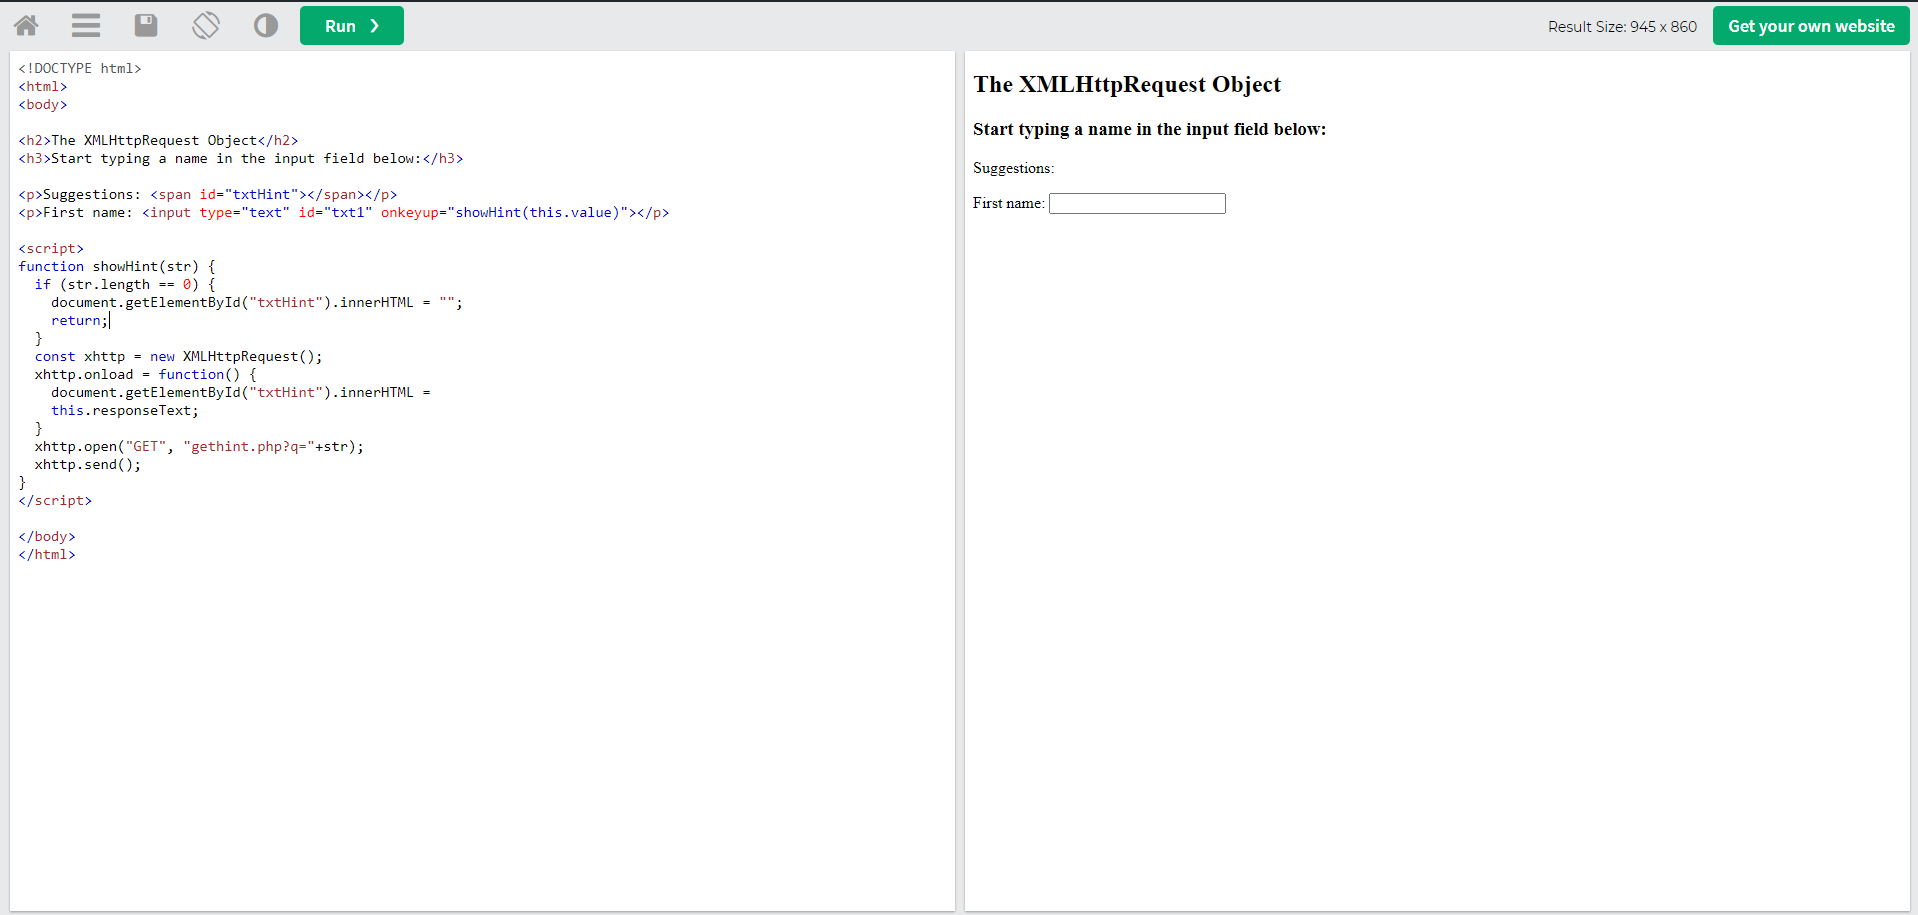
\includegraphics[width=1\textwidth,keepaspectratio]{img/ejemplo15.png}
			\caption{Ajax PHP}
		\end{figure}
		\begin{figure}[H]
			\centering
			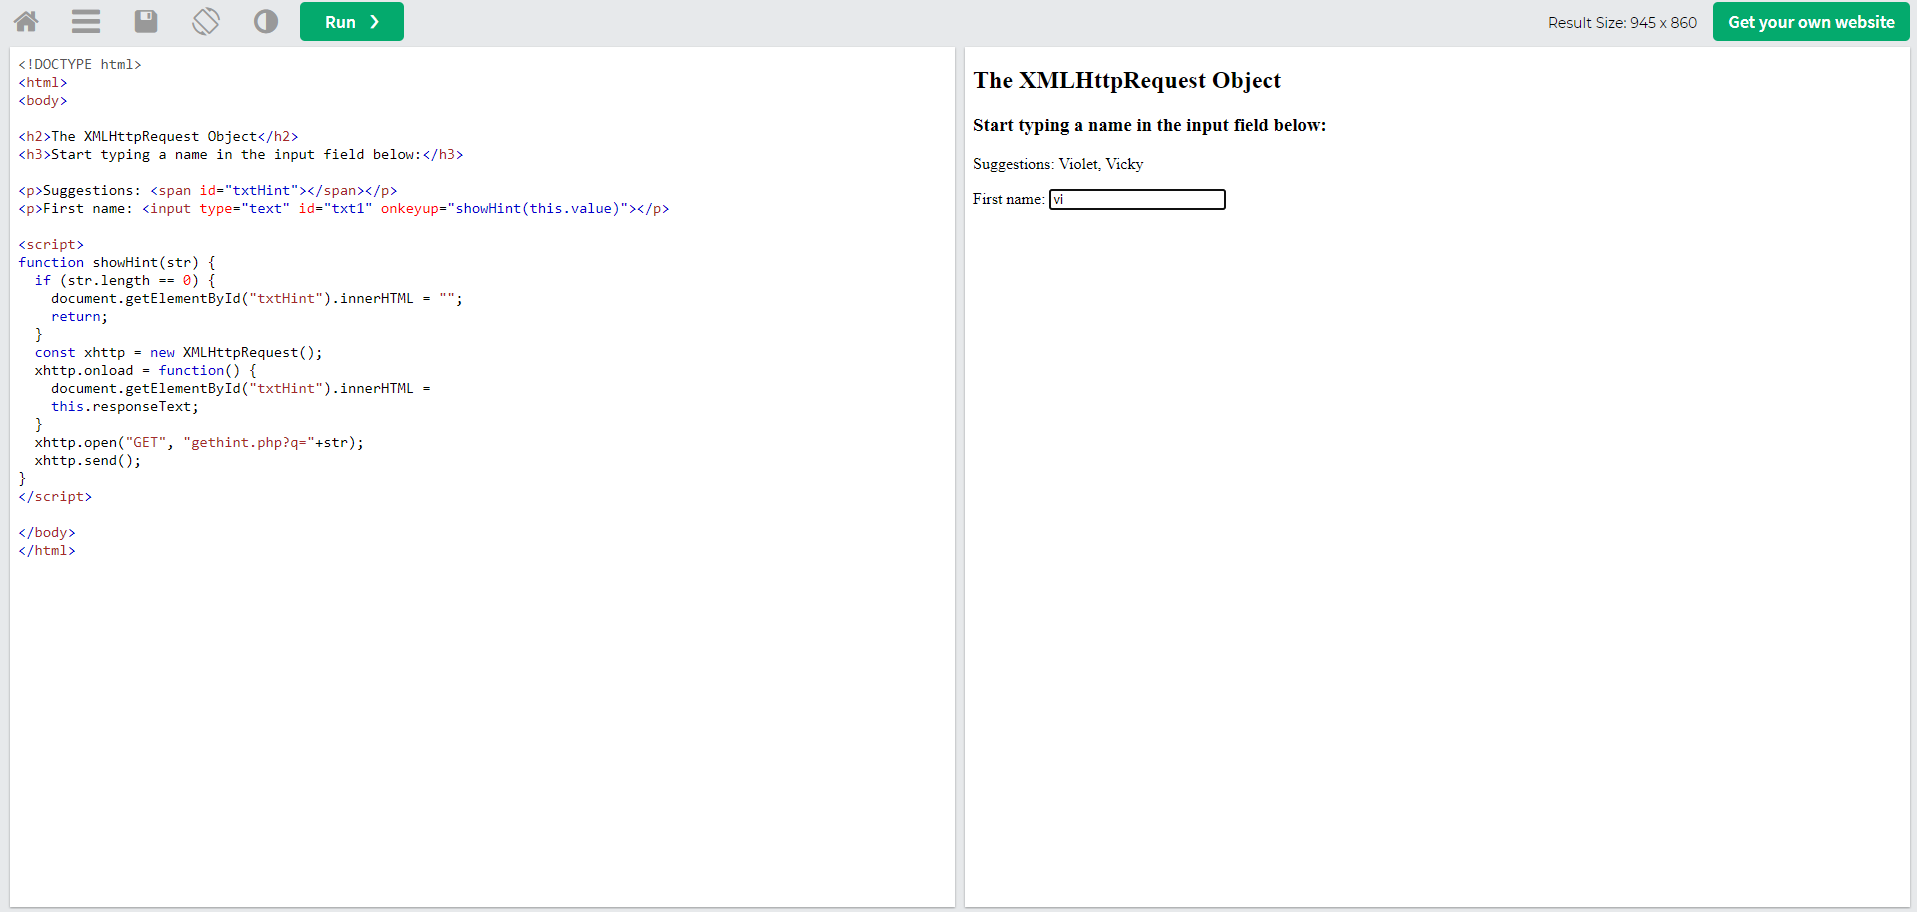
\includegraphics[width=1\textwidth,keepaspectratio]{img/boton15.png}
			\caption{Escribiendo en el cuadro de texto}
		\end{figure}
	\end{itemize}
	\newpage
%%%%%%%%%%%%%%%%%%%%

	\subsubsection{AJAX ASP}
	\begin{itemize}
		\item \textbf{AJAX ASP EXAMPLE}
		\begin{figure}[H]
			\centering
			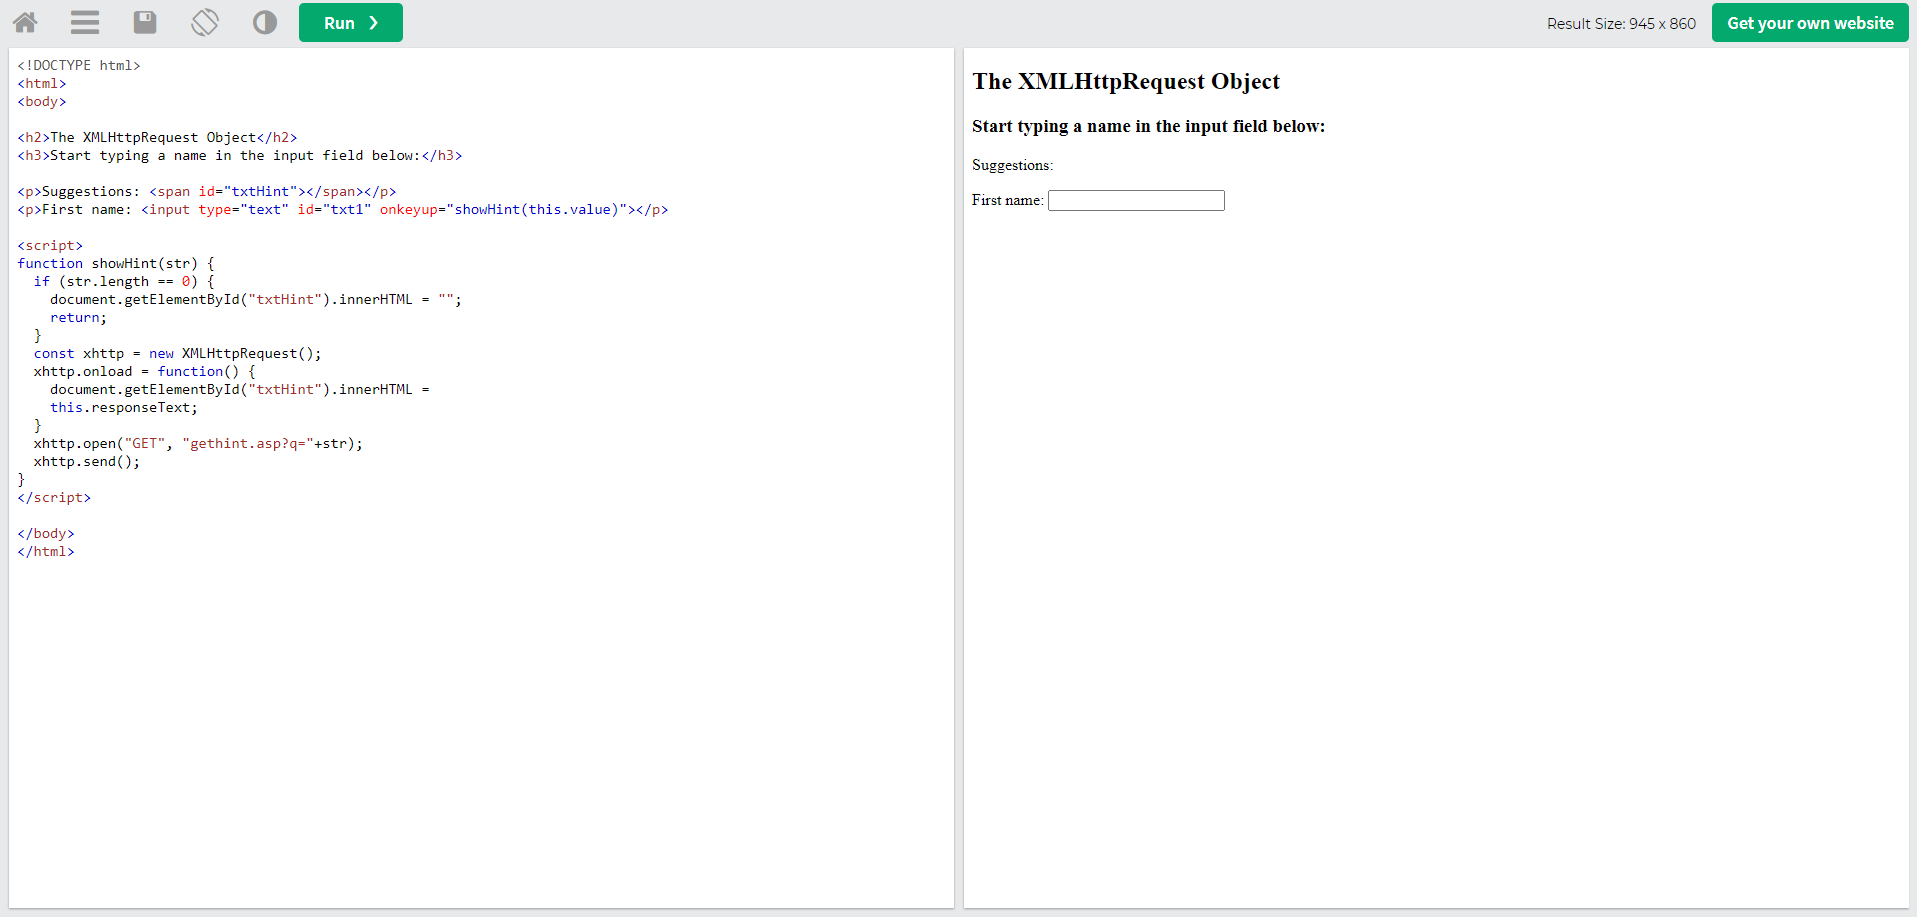
\includegraphics[width=1\textwidth,keepaspectratio]{img/ejemplo16.png}
			\caption{Ajax ASP Example}
		\end{figure}
		\begin{figure}[H]
			\centering
			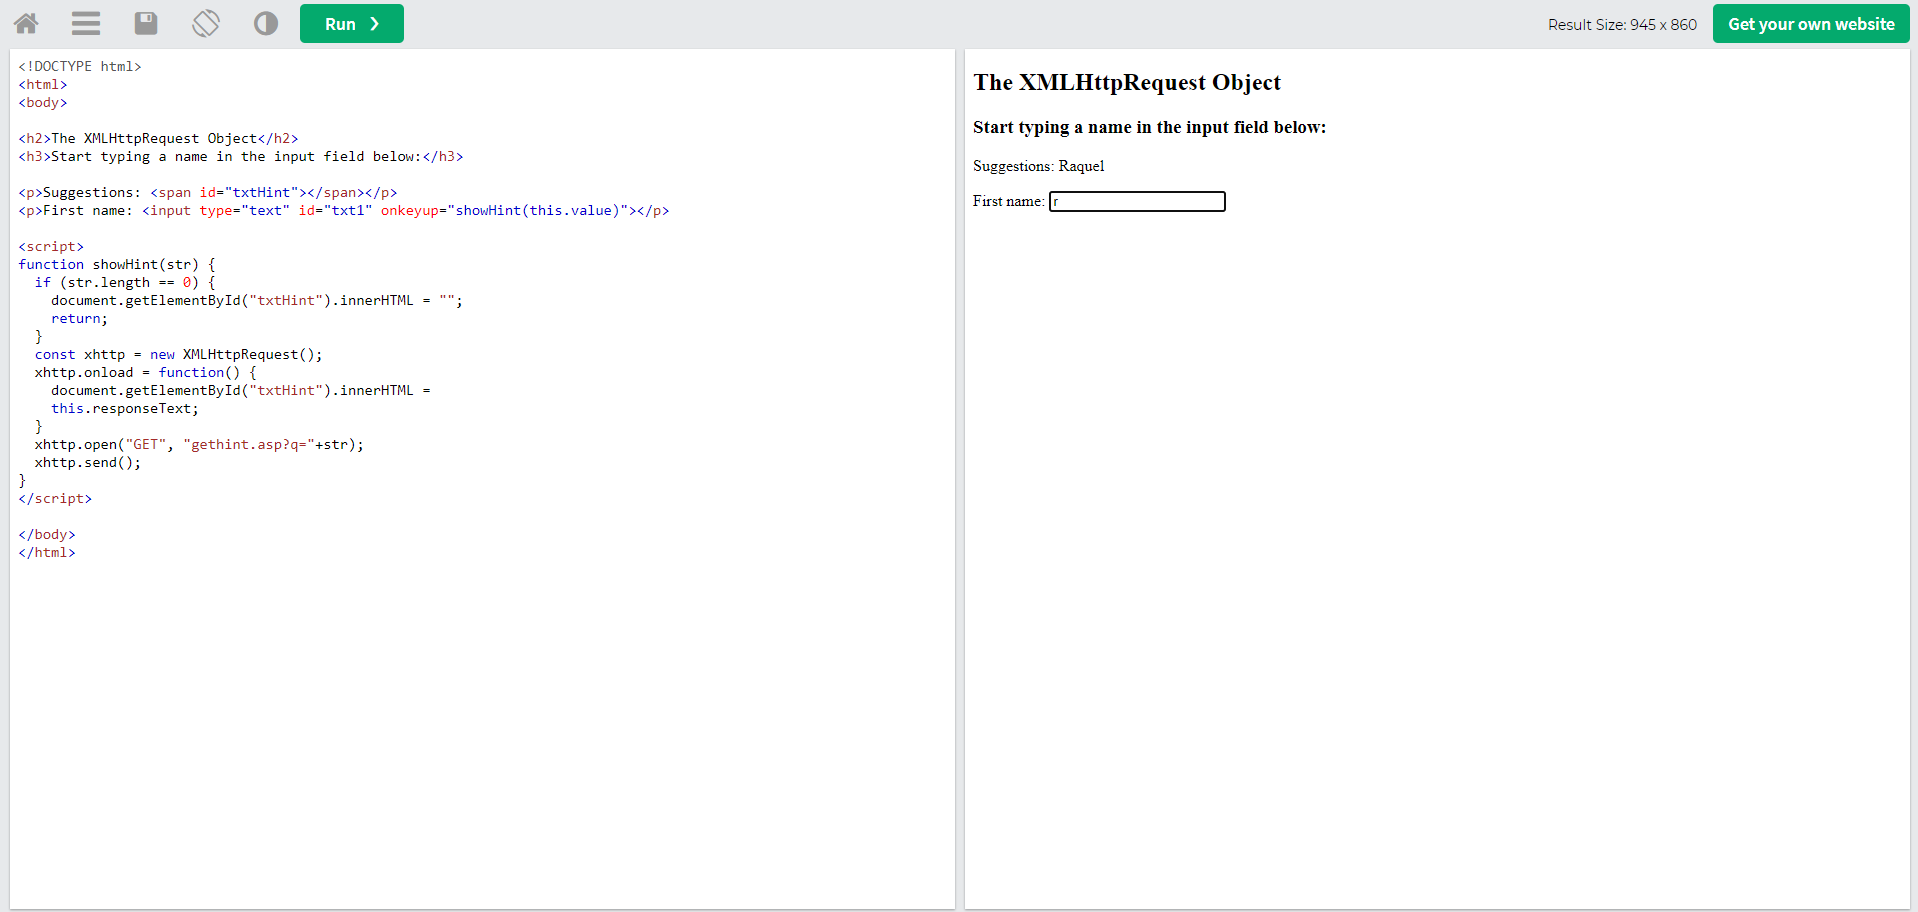
\includegraphics[width=1\textwidth,keepaspectratio]{img/boton16.png}
			\caption{Escribiendo en el cuadro de texto}
		\end{figure}
	\end{itemize}
	\newpage
%%%%%%%%%%%%%%%%%%%%
	
	\subsubsection{AJAX DATABASE}
	\begin{itemize}
		\item \textbf{AJAX ASP EXAMPLE}
		\begin{figure}[H]
			\centering
			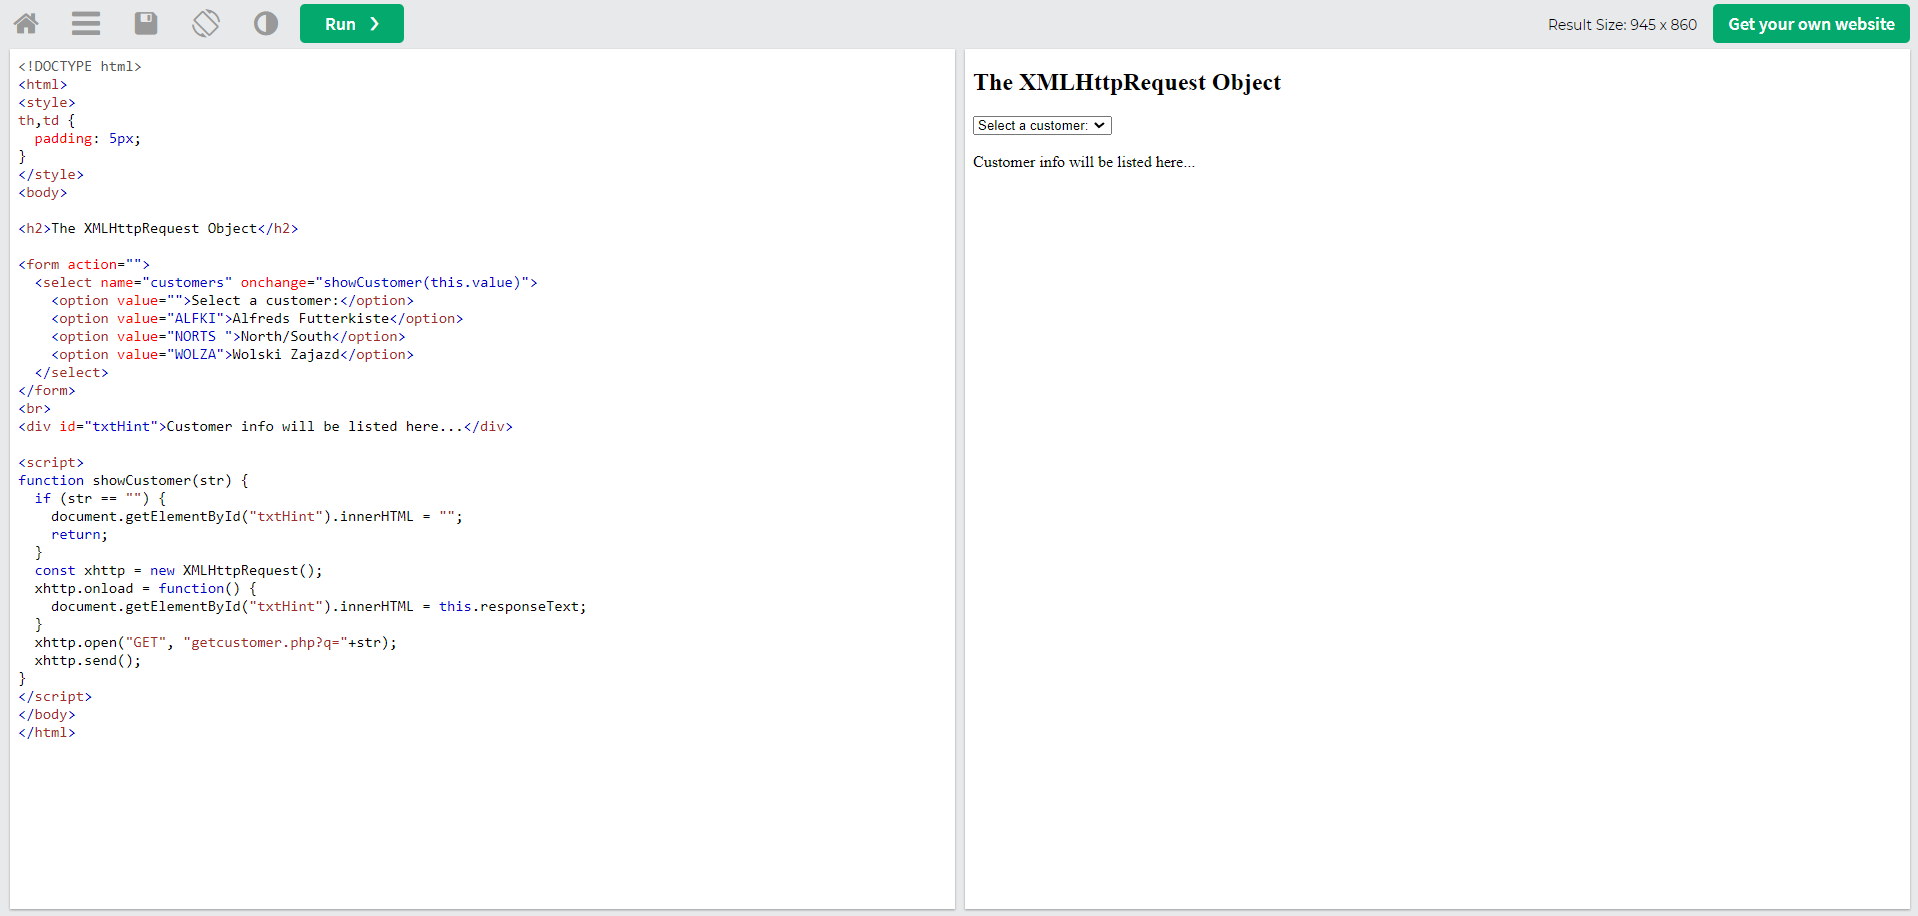
\includegraphics[width=1\textwidth,keepaspectratio]{img/ejemplo17.png}
			\caption{Ajax Database Example}
		\end{figure}
		\begin{figure}[H]
			\centering
			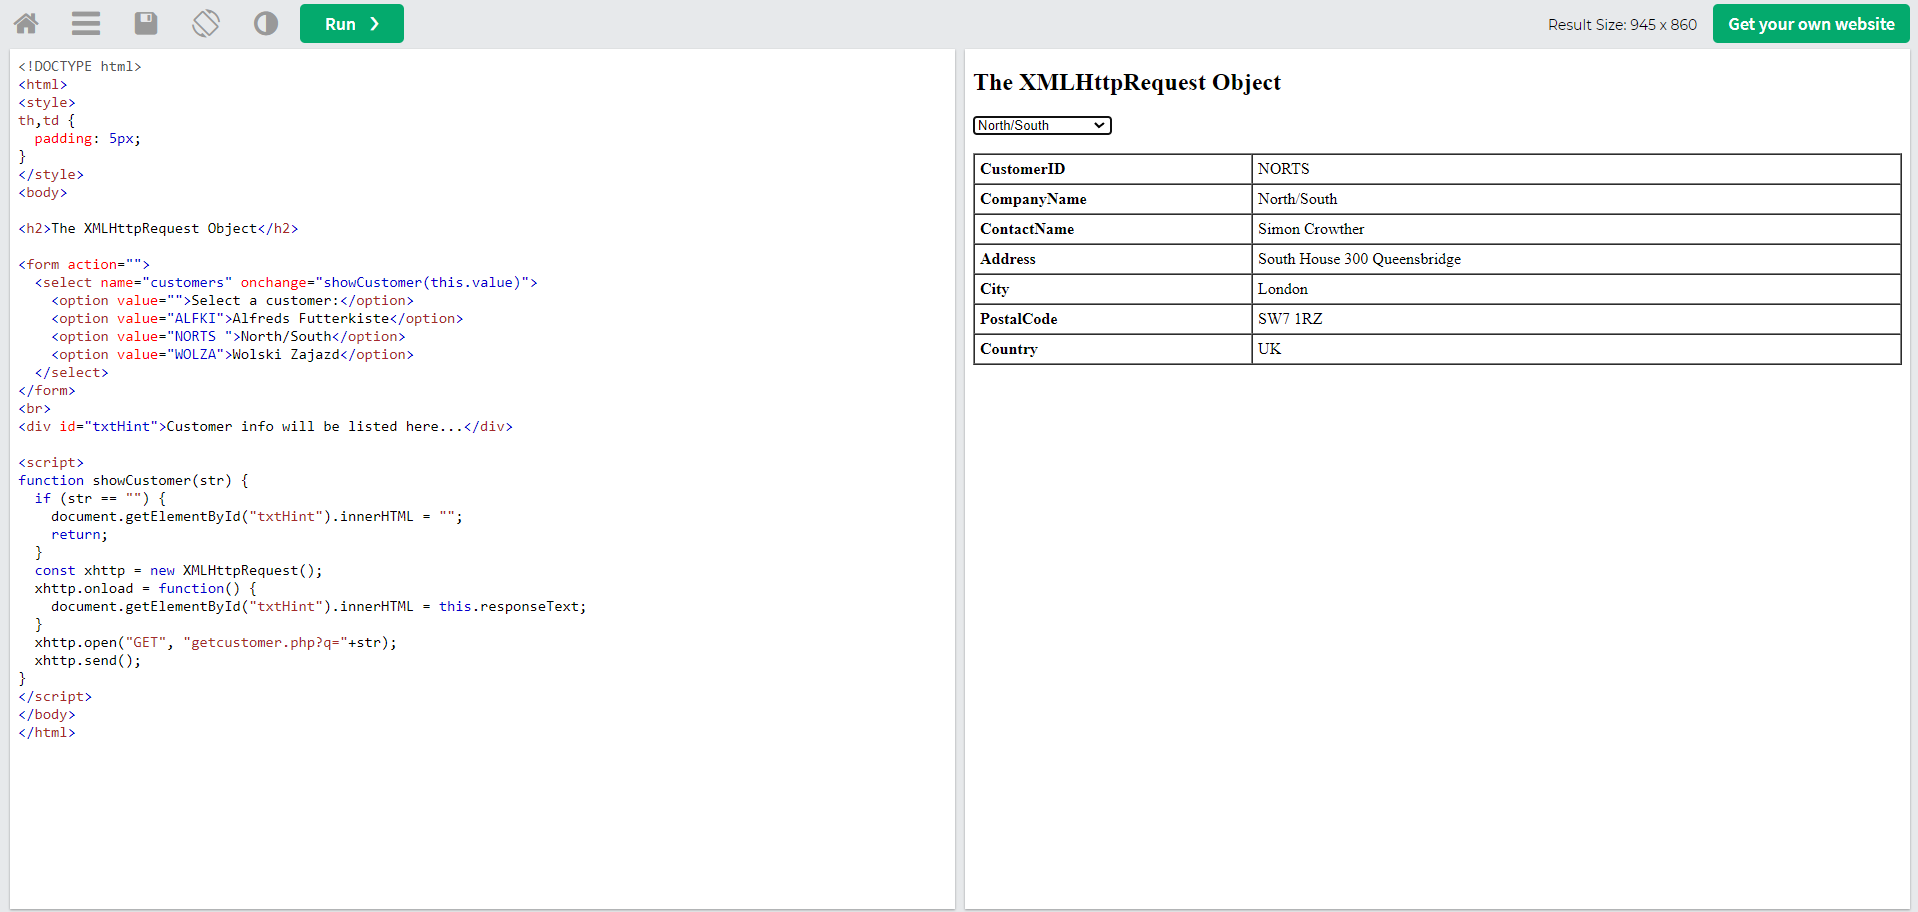
\includegraphics[width=1\textwidth,keepaspectratio]{img/seleccion1.png}
			\caption{Eligiendo una opción}
		\end{figure}
	\end{itemize}
	\newpage
%%%%%%%%%%%%%%%%%%%%
	\subsubsection{AJAX - Applications}
	\begin{itemize}
		\item \textbf{Mostrar datos XML en una tabla HTML}
		\begin{figure}[H]
			\centering
			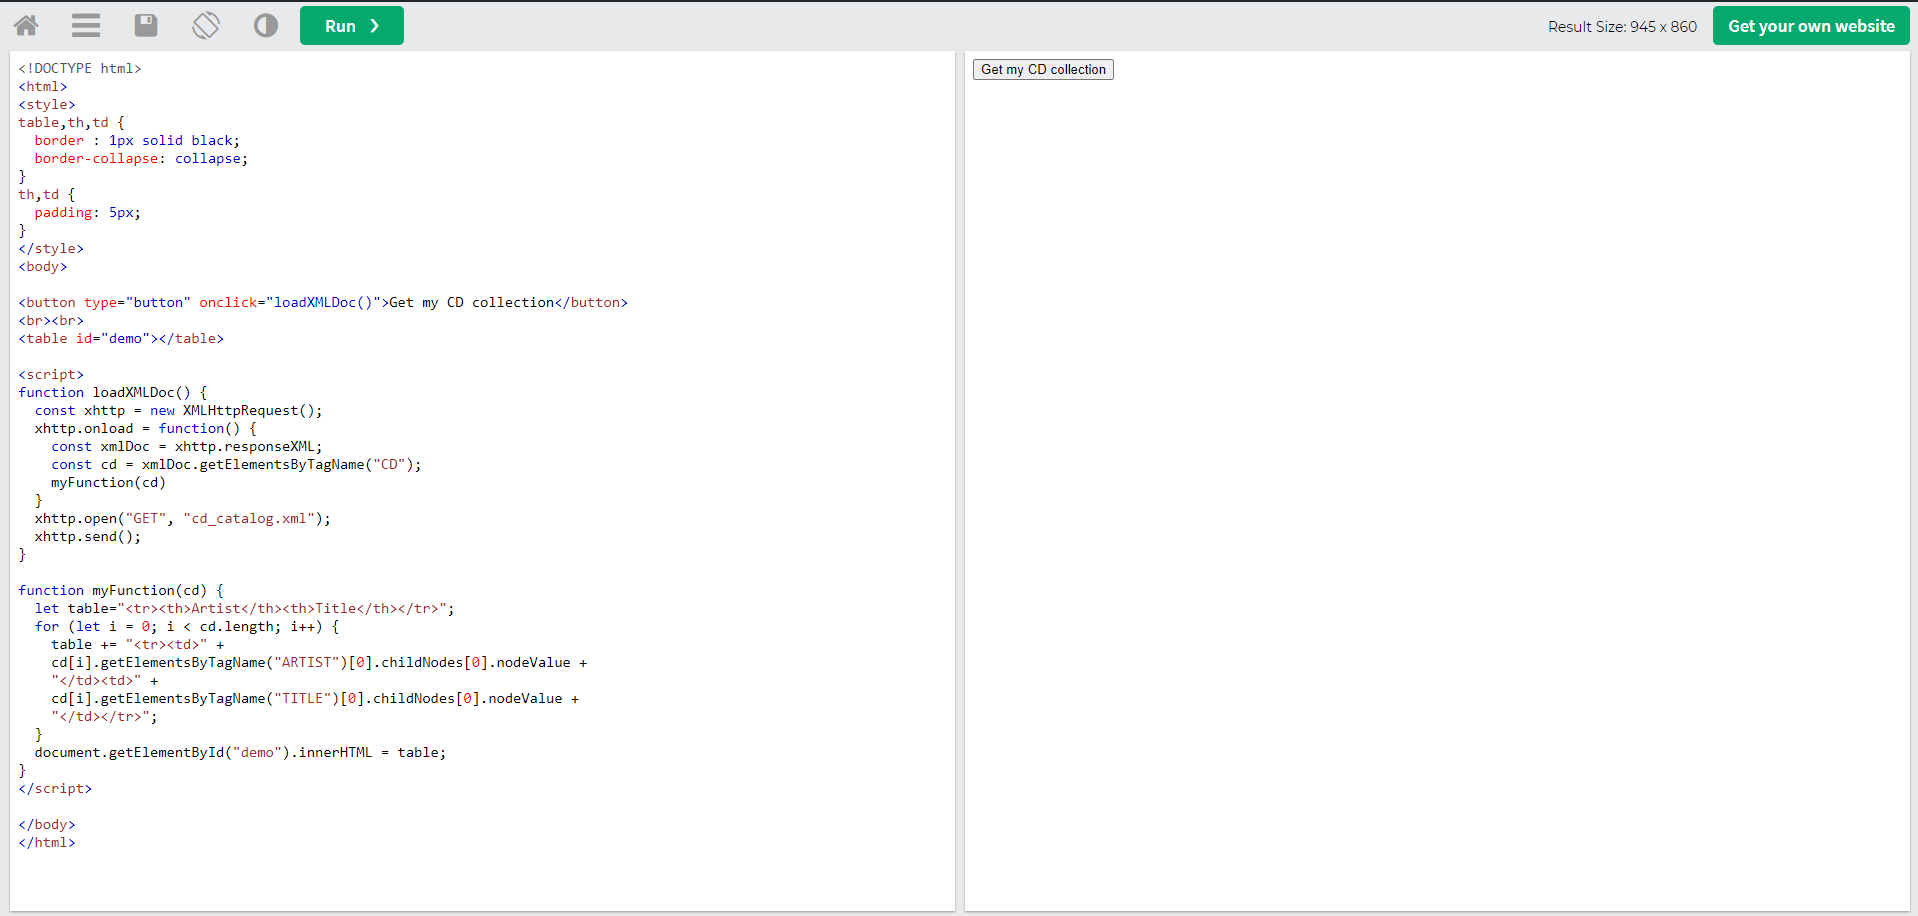
\includegraphics[width=1\textwidth,keepaspectratio]{img/ejemplo18.png}
			\caption{Estructura}
		\end{figure}
		\begin{figure}[H]
			\centering
			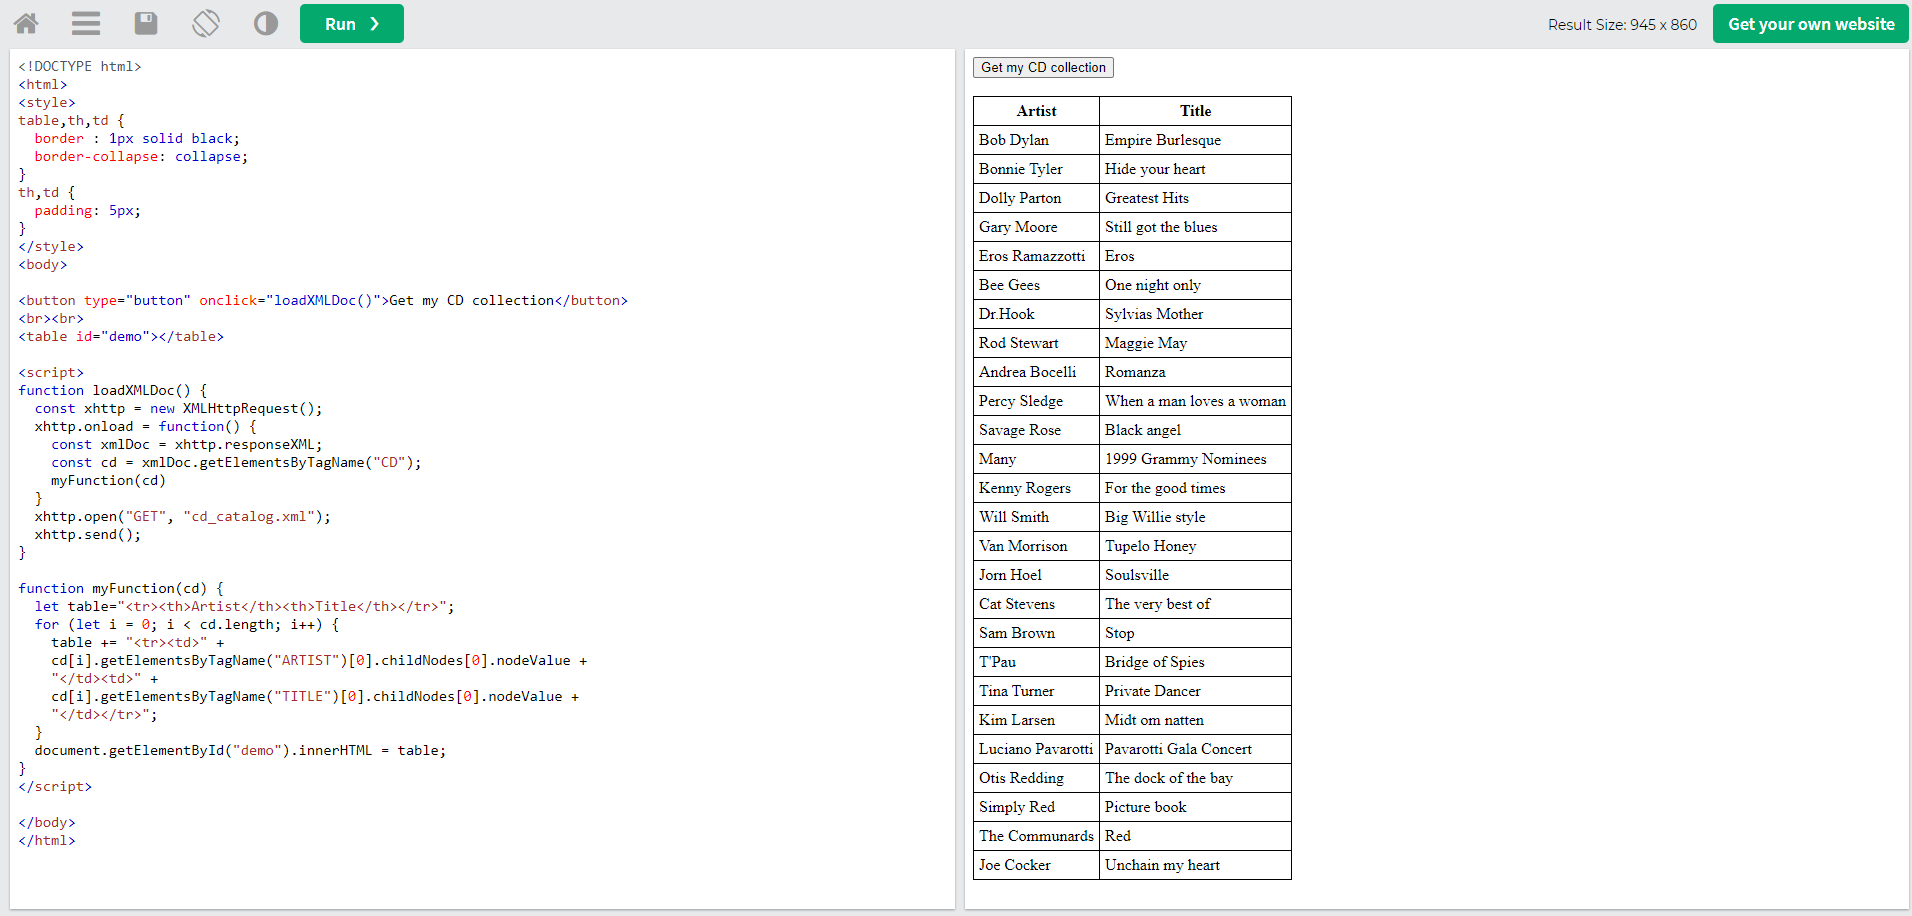
\includegraphics[width=1\textwidth,keepaspectratio]{img/boton18.png}
			\caption{Mostrar Datos}
		\end{figure}
		\newpage
		\item \textbf{Mostrar el primer CD en un elemento div HTML}
		\begin{figure}[H]
			\centering
			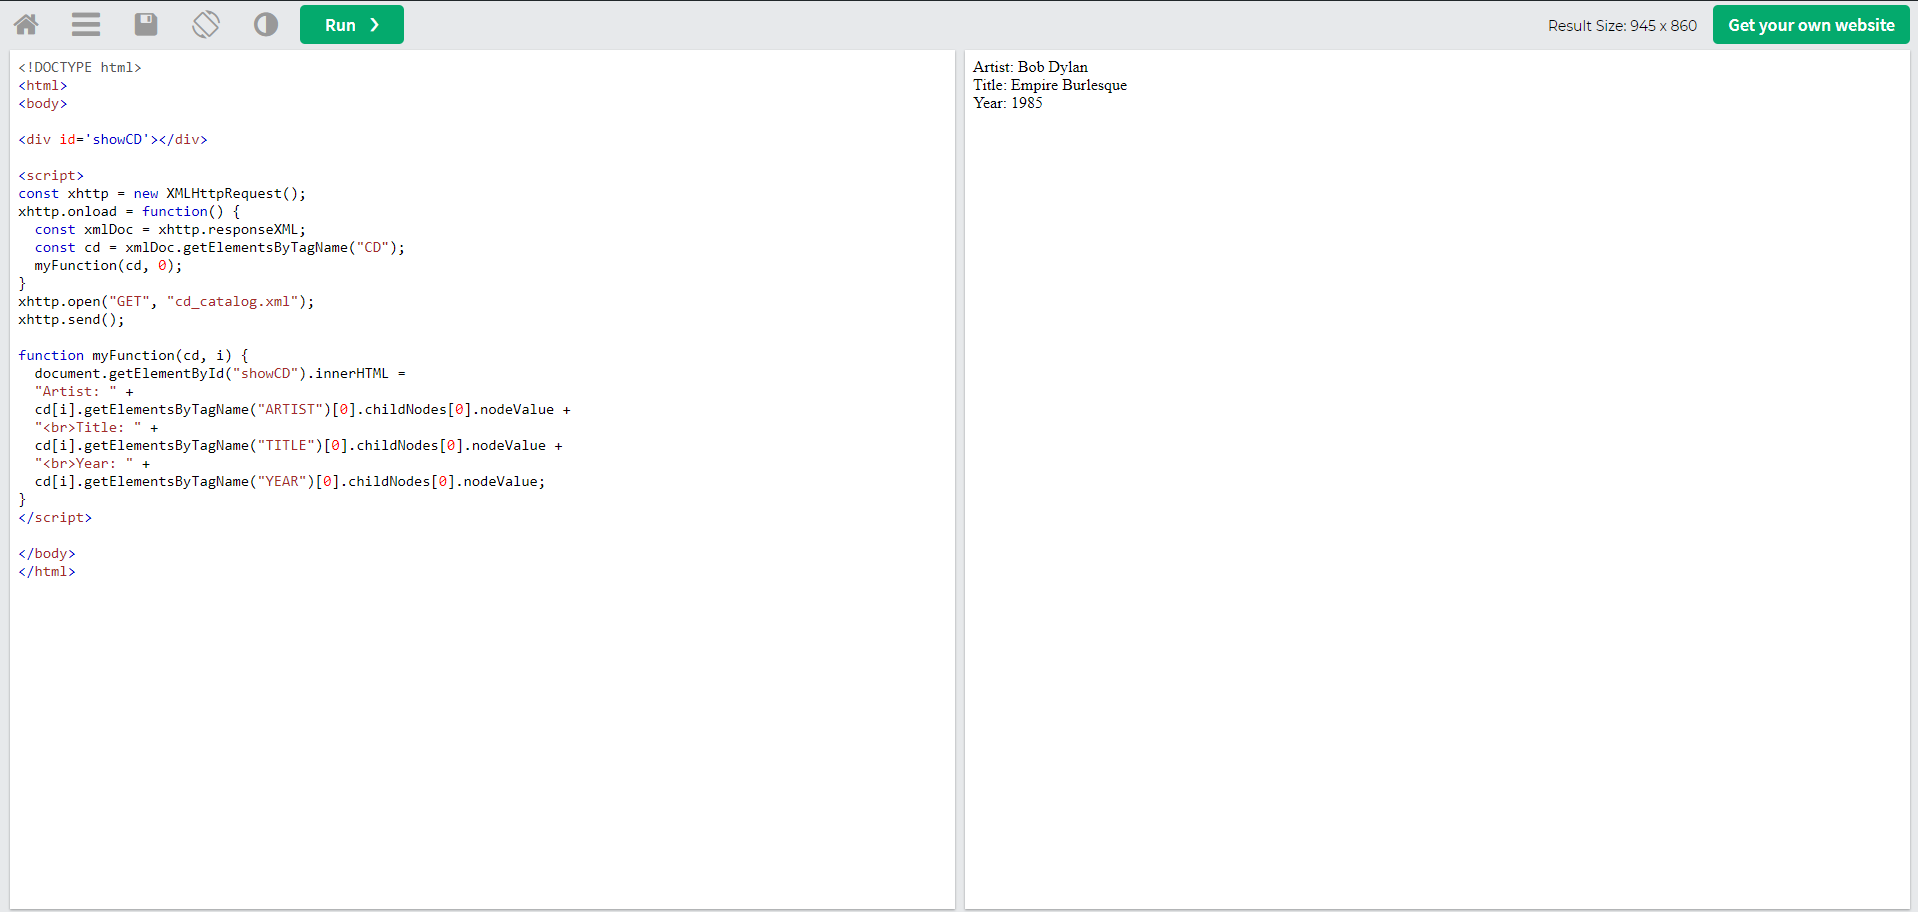
\includegraphics[width=1\textwidth,keepaspectratio]{img/ejemplo19.png}
			\caption{Mostrar primer elemento}
		\end{figure}
		\item \textbf{Navegar entre los CD}
		\begin{figure}[H]
			\centering
			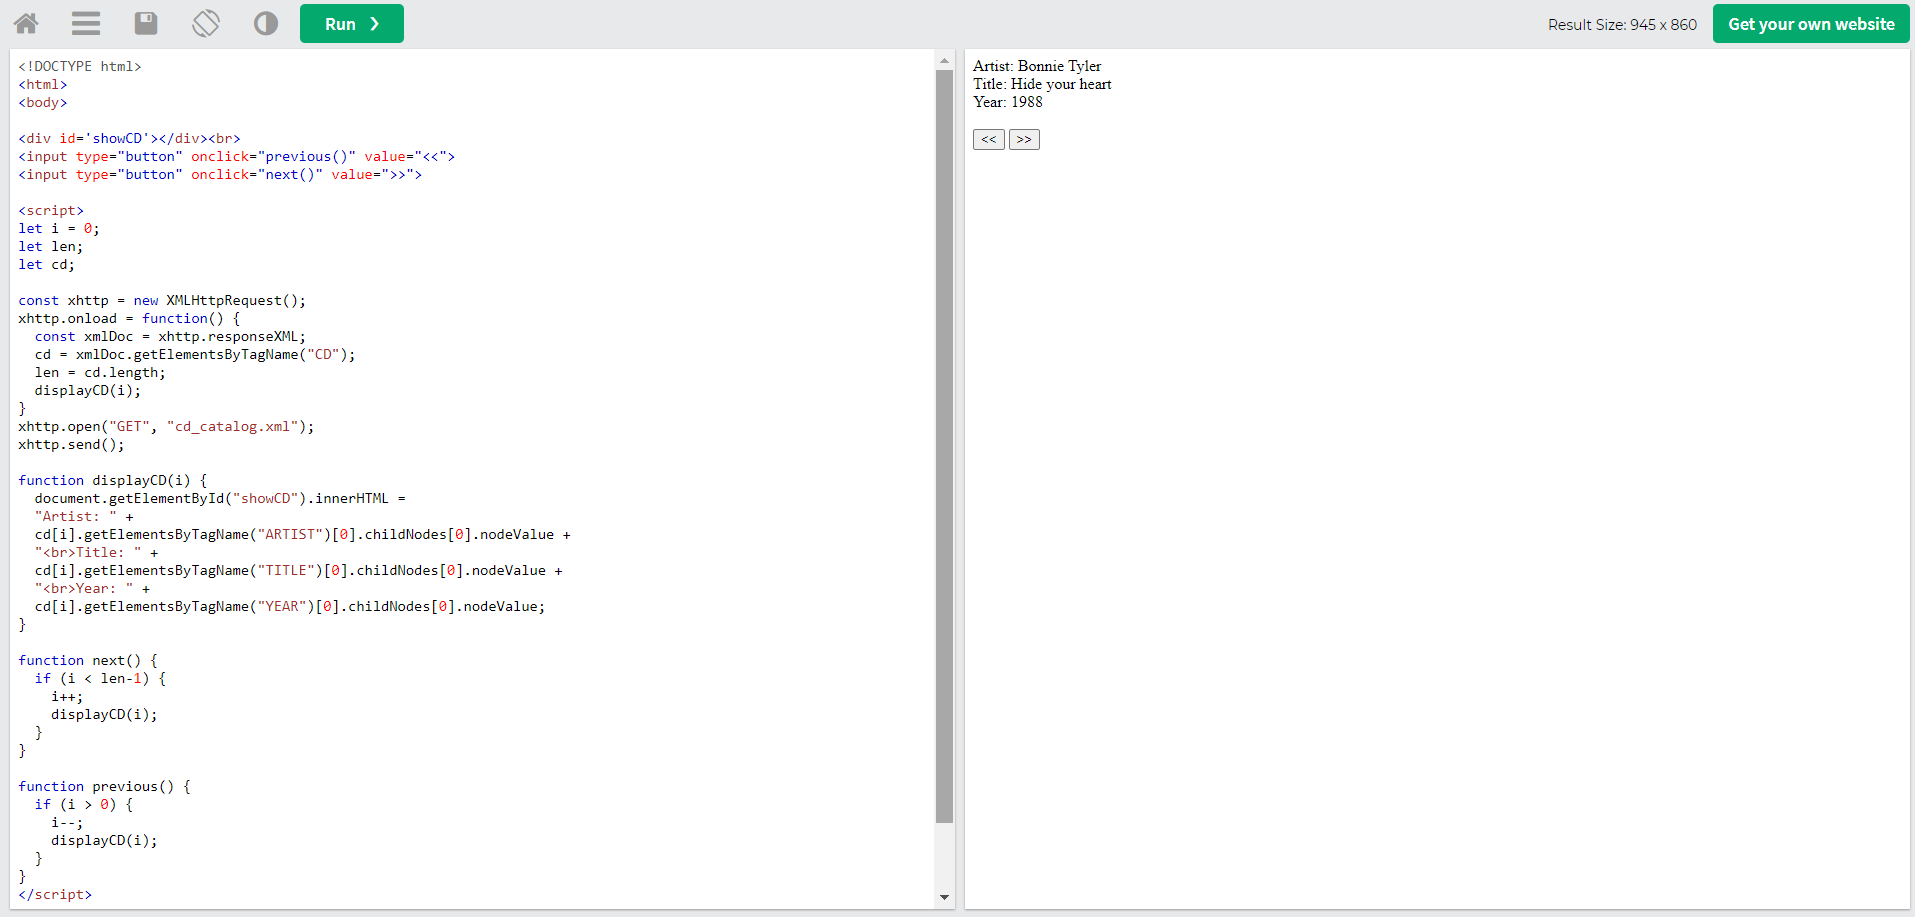
\includegraphics[width=1\textwidth,keepaspectratio]{img/ejemplo20.png}
			\caption{Navegar entre CD}
		\end{figure}
		\newpage
		\item \textbf{Mostrar información del álbum al hacer clic en un CD}
		\begin{figure}[H]
			\centering
			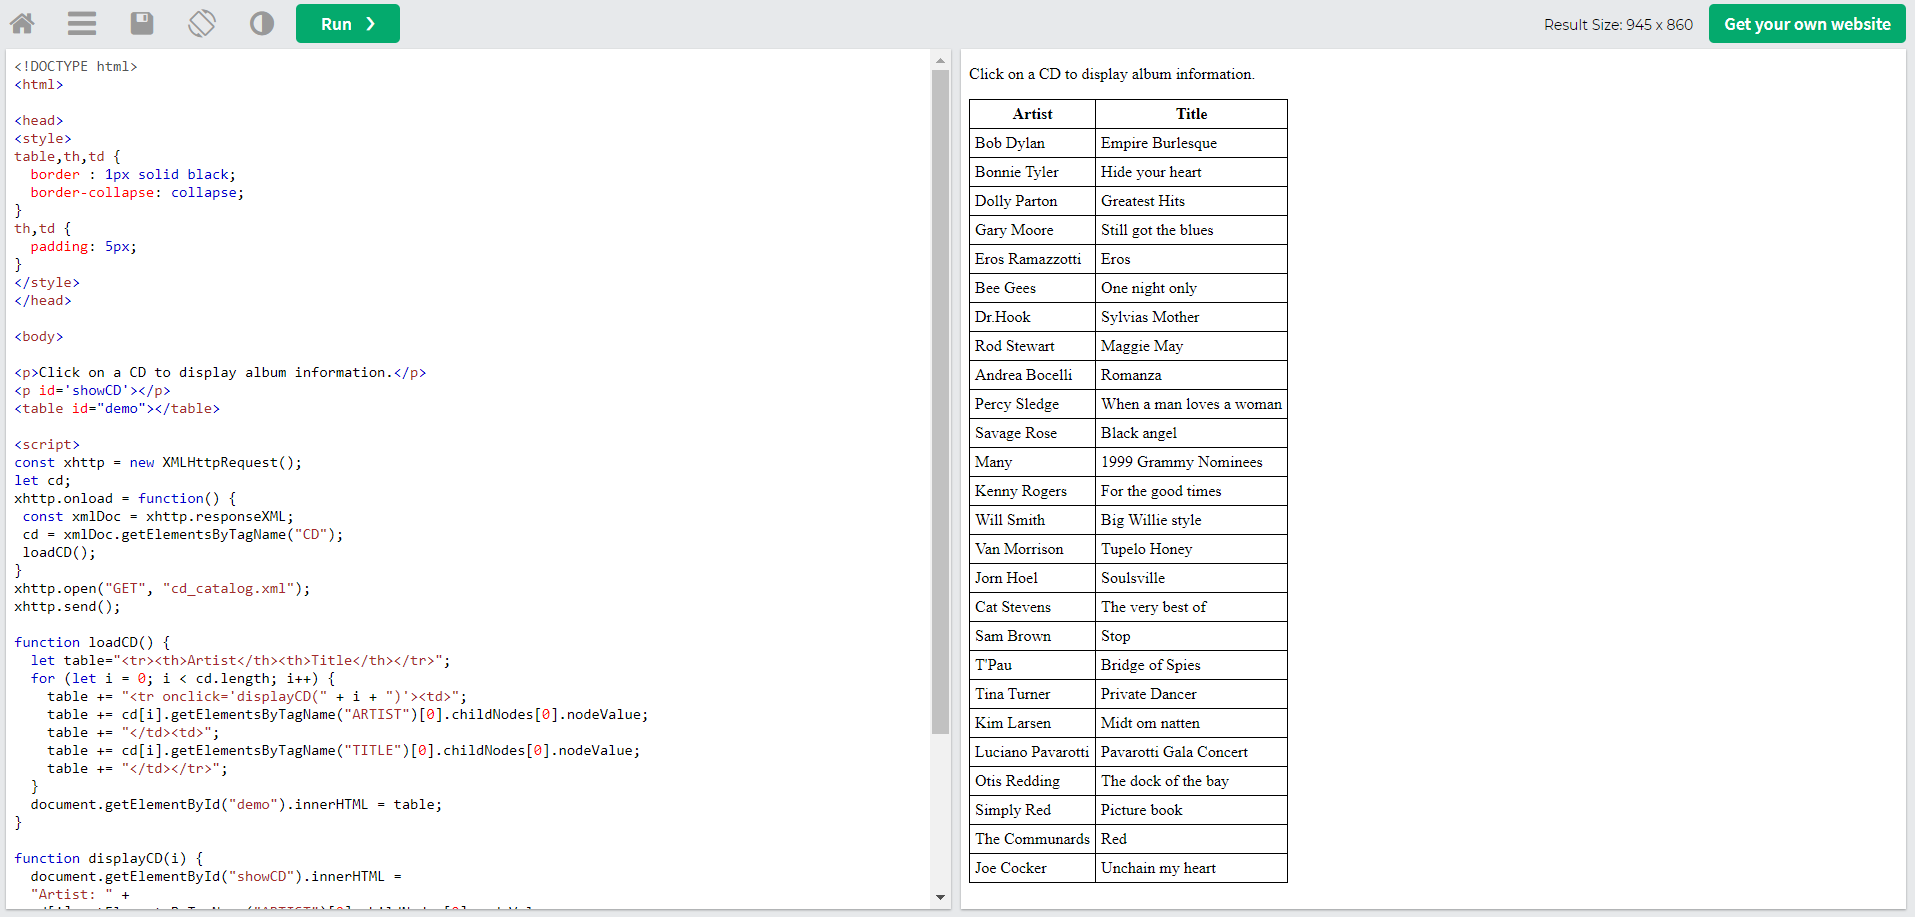
\includegraphics[width=1\textwidth,keepaspectratio]{img/ejemplo21.png}
			\caption{Mostrar tabla de CD}
		\end{figure}
		\begin{figure}[H]
			\centering
			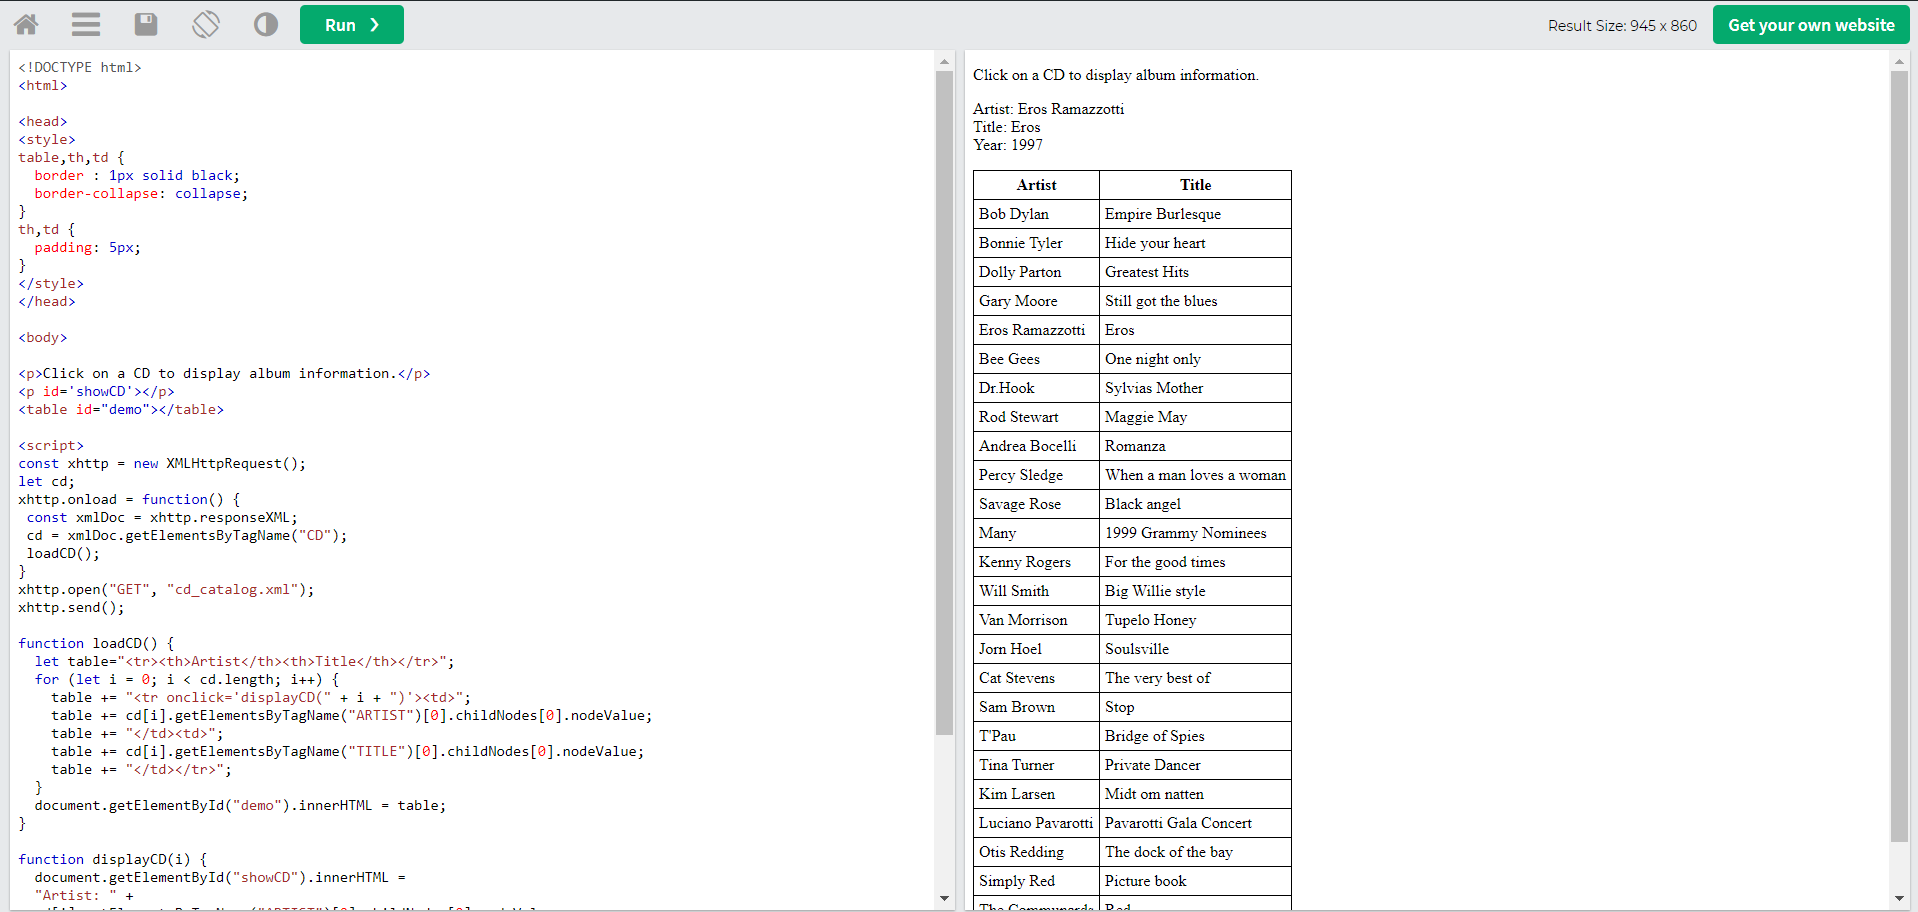
\includegraphics[width=1\textwidth,keepaspectratio]{img/seleccion2.png}
			\caption{Haciendo Click en un CD}
		\end{figure}
	\end{itemize}
	\newpage
%%%%%%%%%%%%%%%%%%%%
	\subsubsection{AJAX - Examples}
	\begin{itemize}
		\item \textbf{SIMPLES EXAMPLES}
		\begin{figure}[H]
			\centering
			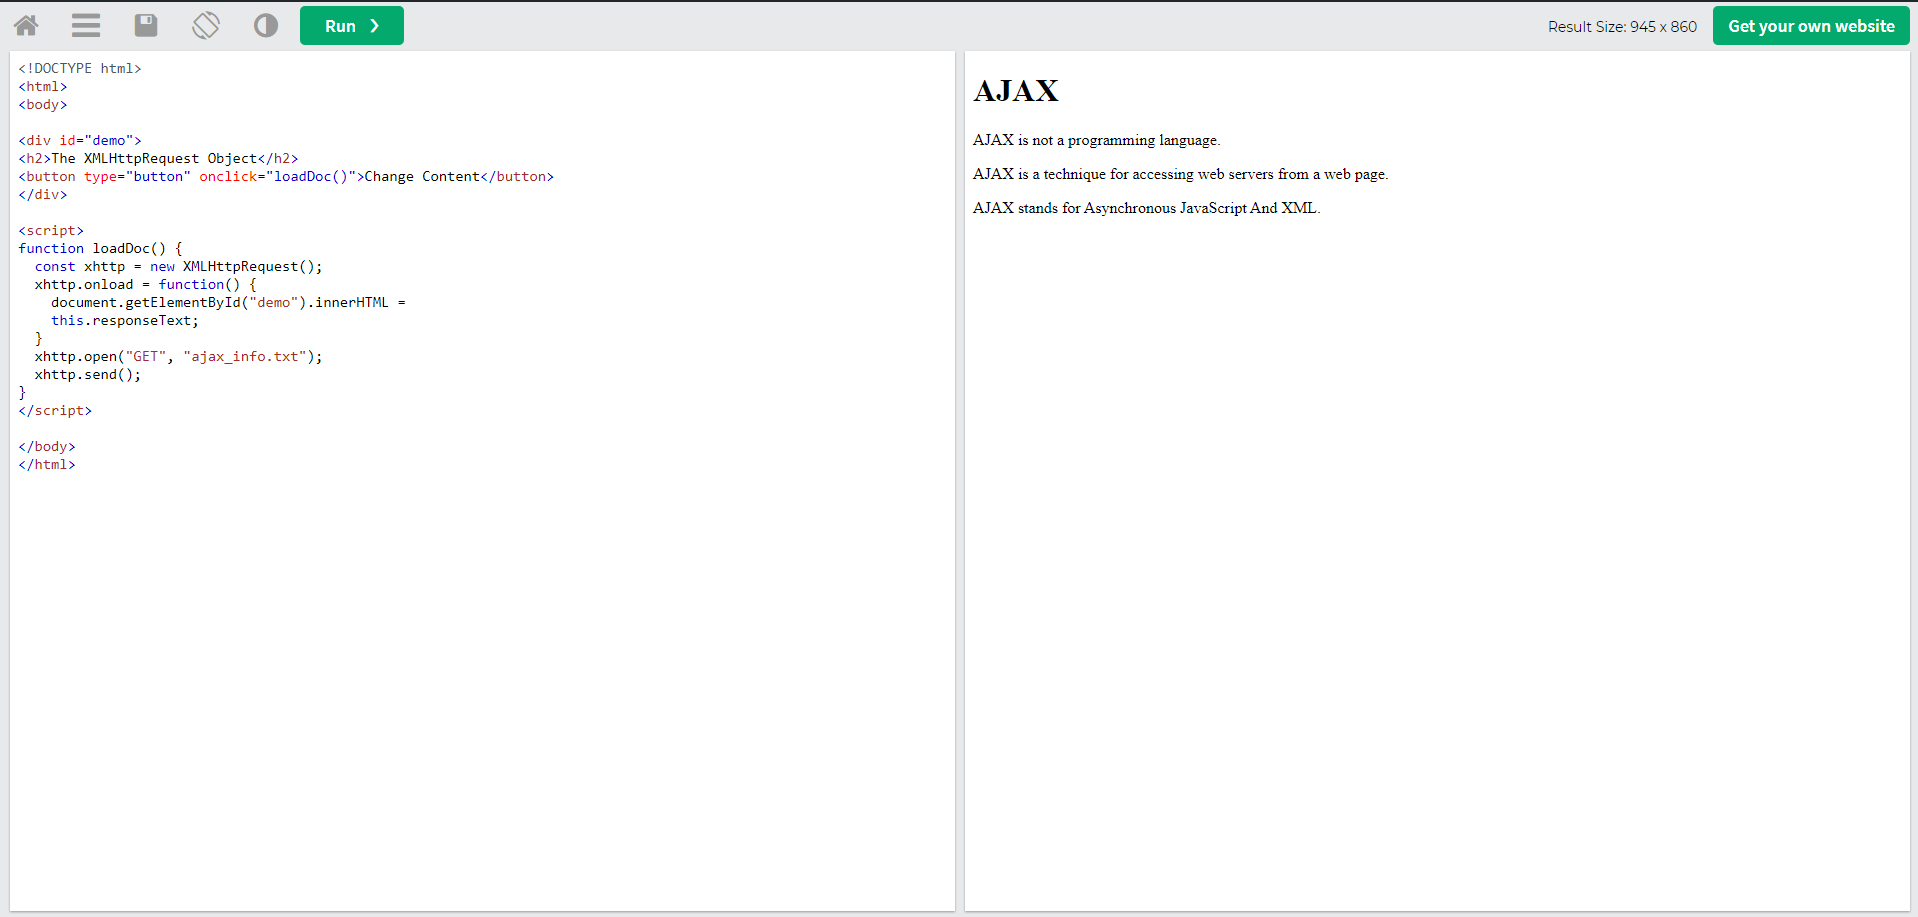
\includegraphics[width=1\textwidth,keepaspectratio]{img/ejemplo22.png}
			\caption{Ejemplo 1}
		\end{figure}
		\begin{figure}[H]
			\centering
			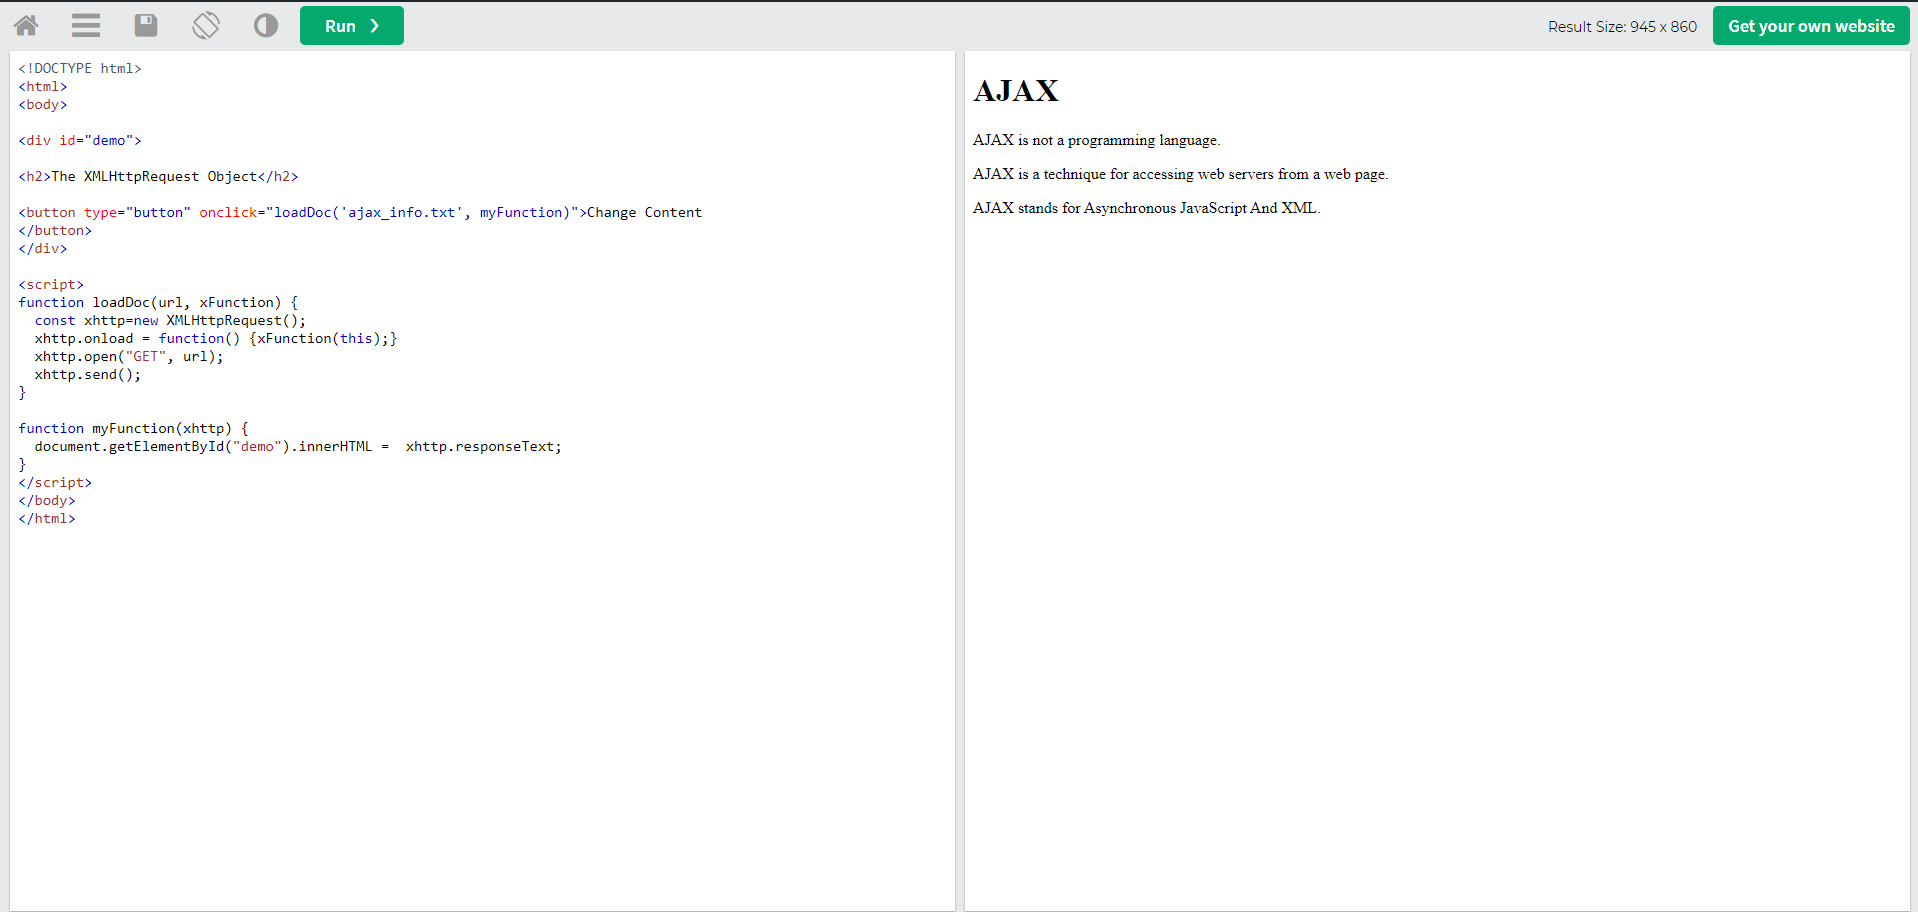
\includegraphics[width=1\textwidth,keepaspectratio]{img/ejemplo23.png}
			\caption{Ejemplo 2}
		\end{figure}
		\newpage
		\item \textbf{Request Header Information}
		\begin{figure}[H]
			\centering
			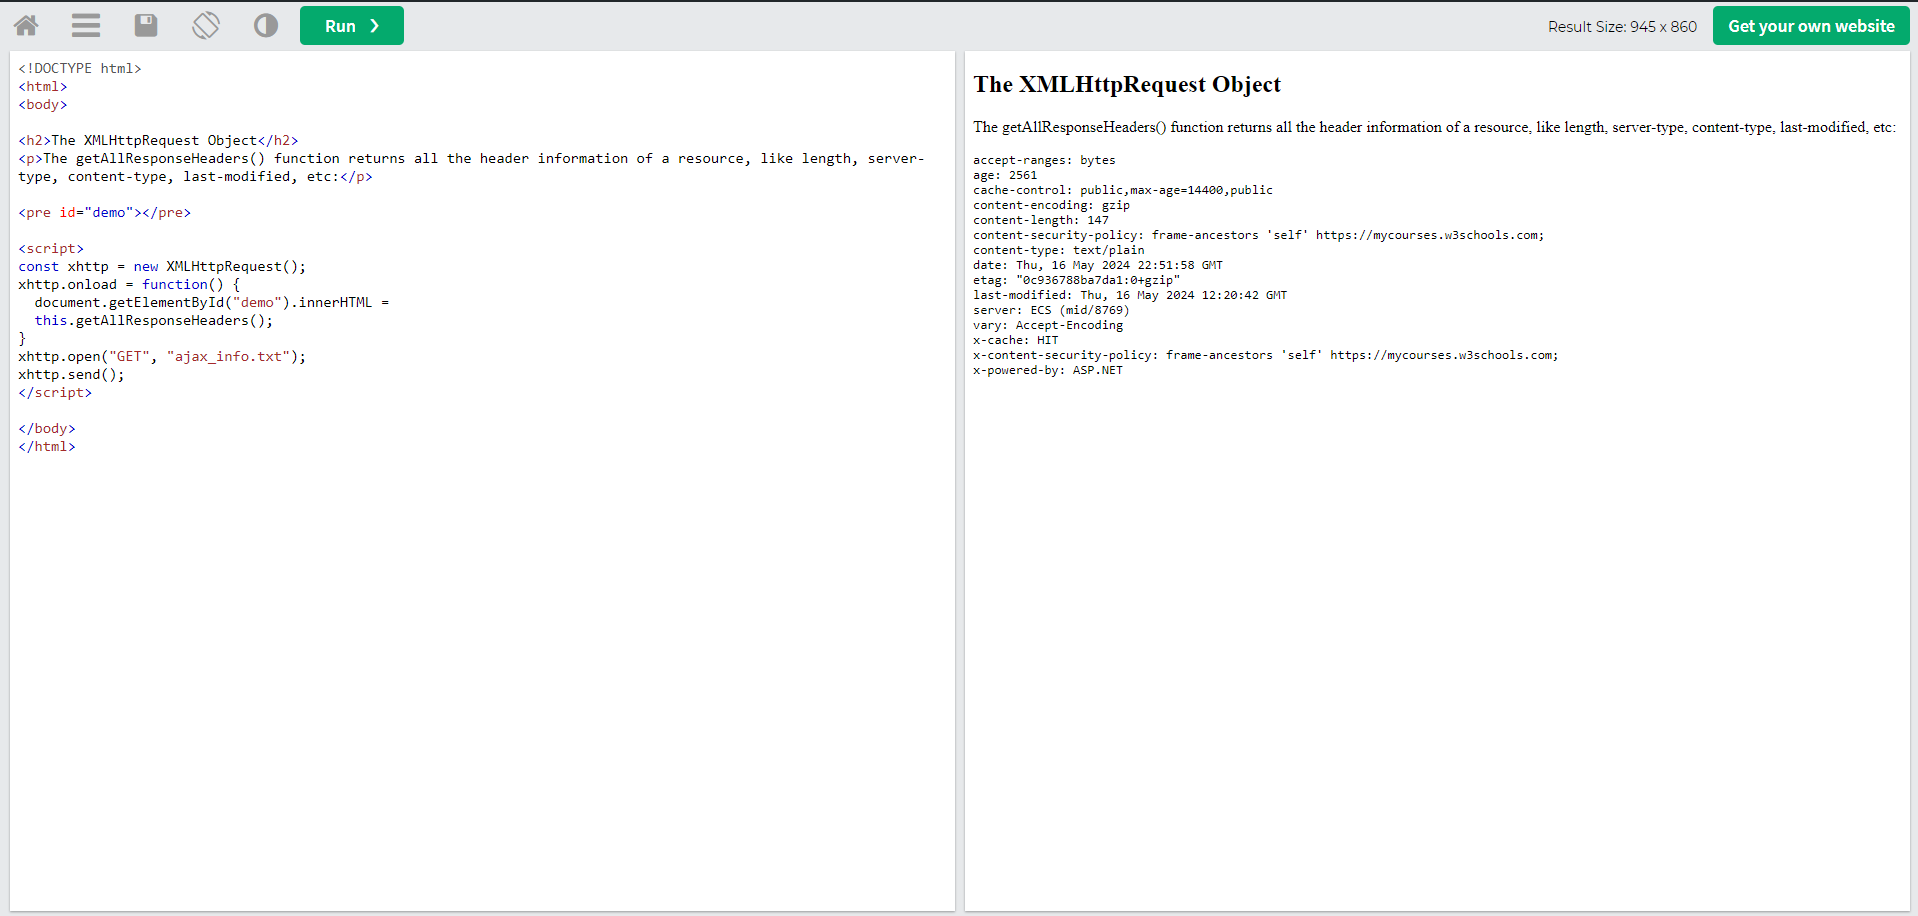
\includegraphics[width=1\textwidth,keepaspectratio]{img/ejemplo24.png}
			\caption{Ejemplo 1}
		\end{figure}
		\begin{figure}[H]
			\centering
			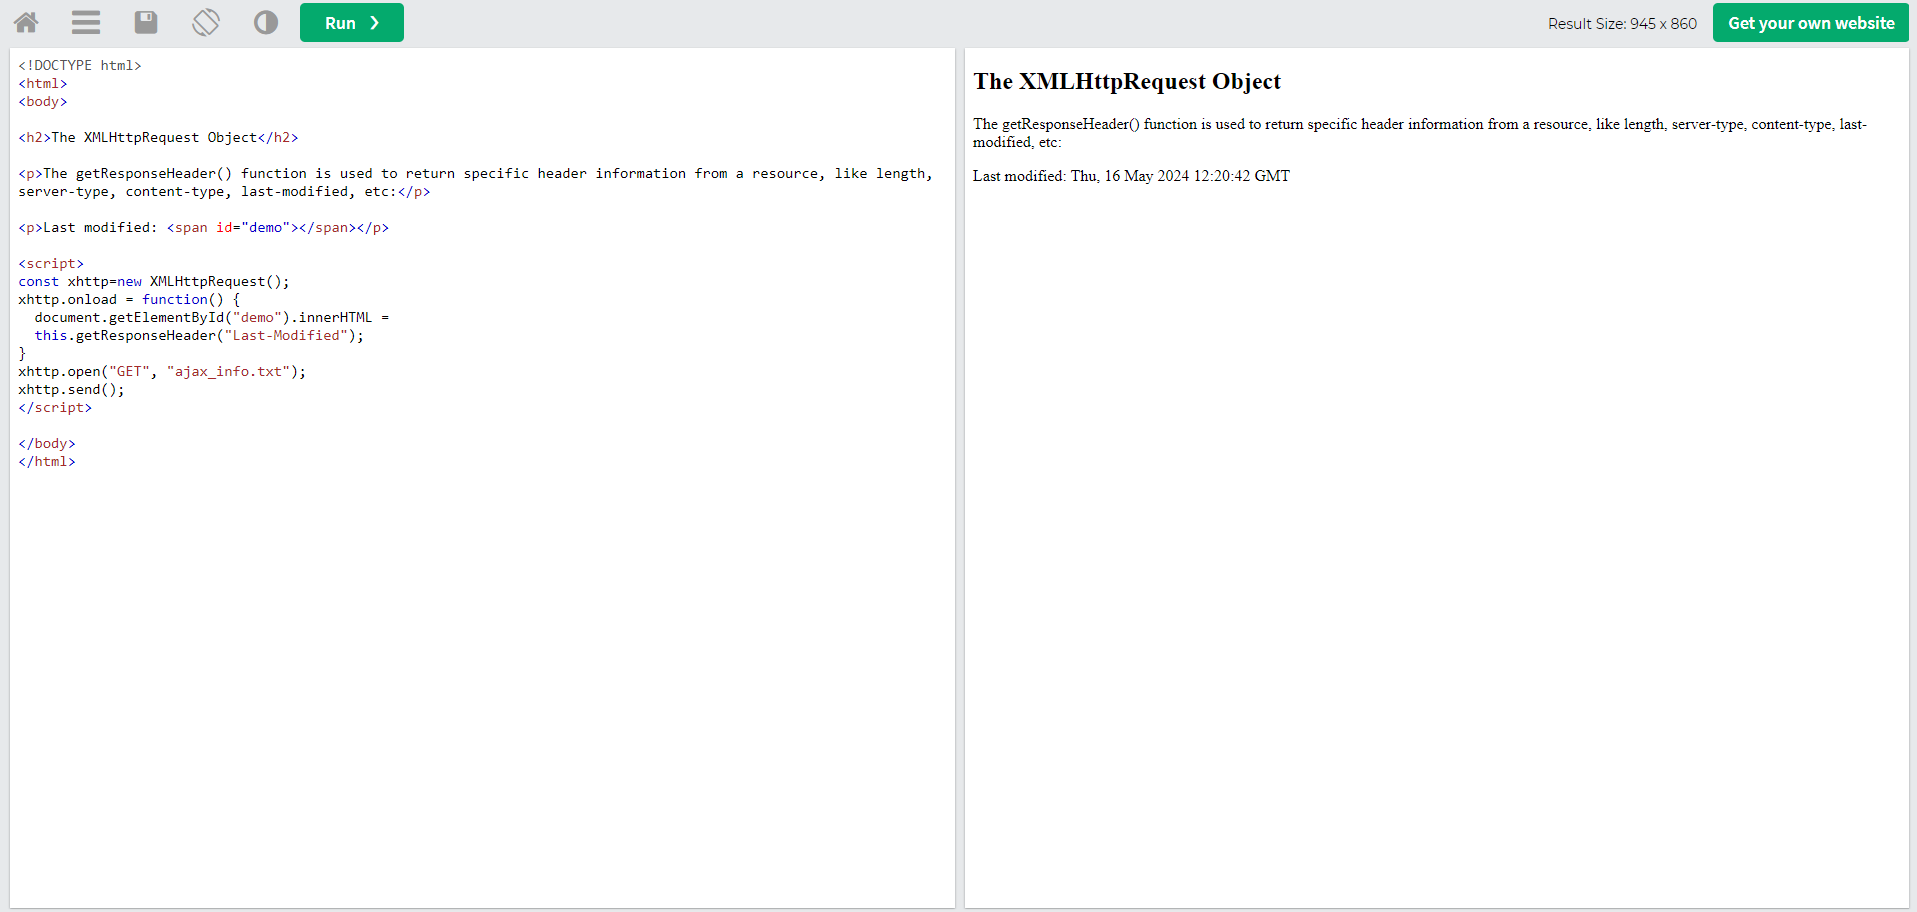
\includegraphics[width=1\textwidth,keepaspectratio]{img/ejemplo25.png}
			\caption{Ejemplo 2}
		\end{figure}
		\newpage
		\item \textbf{Request XML Files}
		\begin{figure}[H]
			\centering
			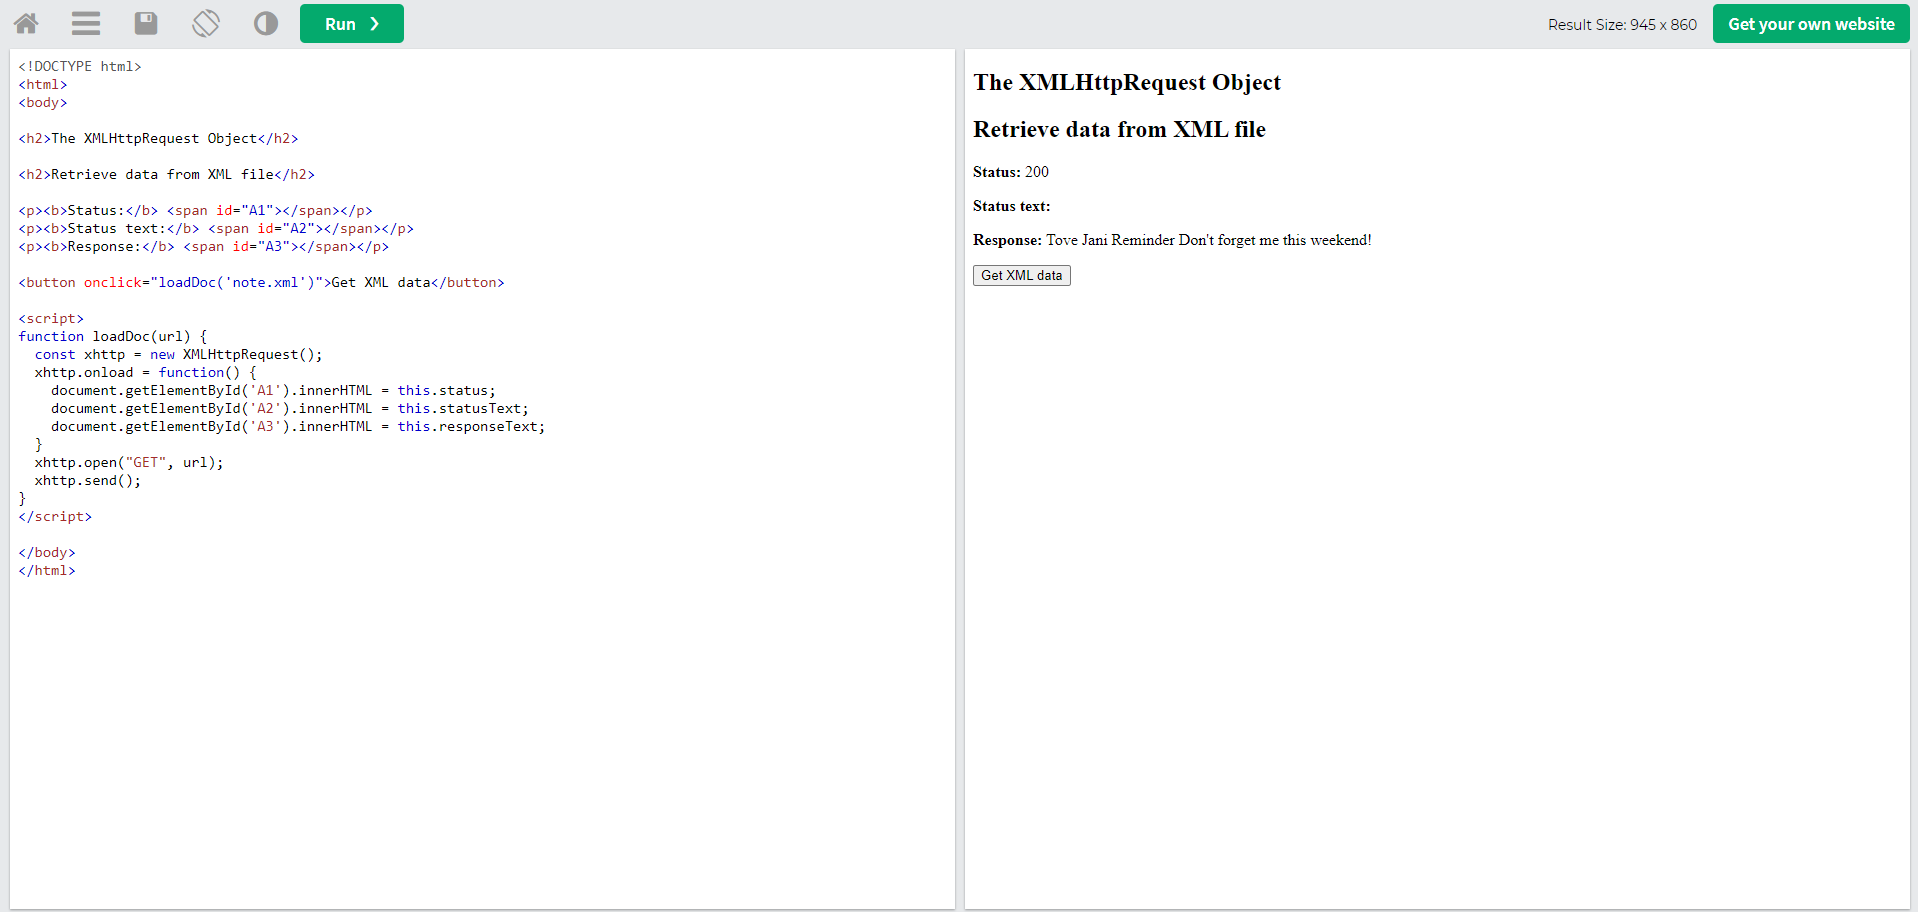
\includegraphics[width=1\textwidth,keepaspectratio]{img/ejemplo26.png}
			\caption{Ejemplo 1}
		\end{figure}
		\begin{figure}[H]
			\centering
			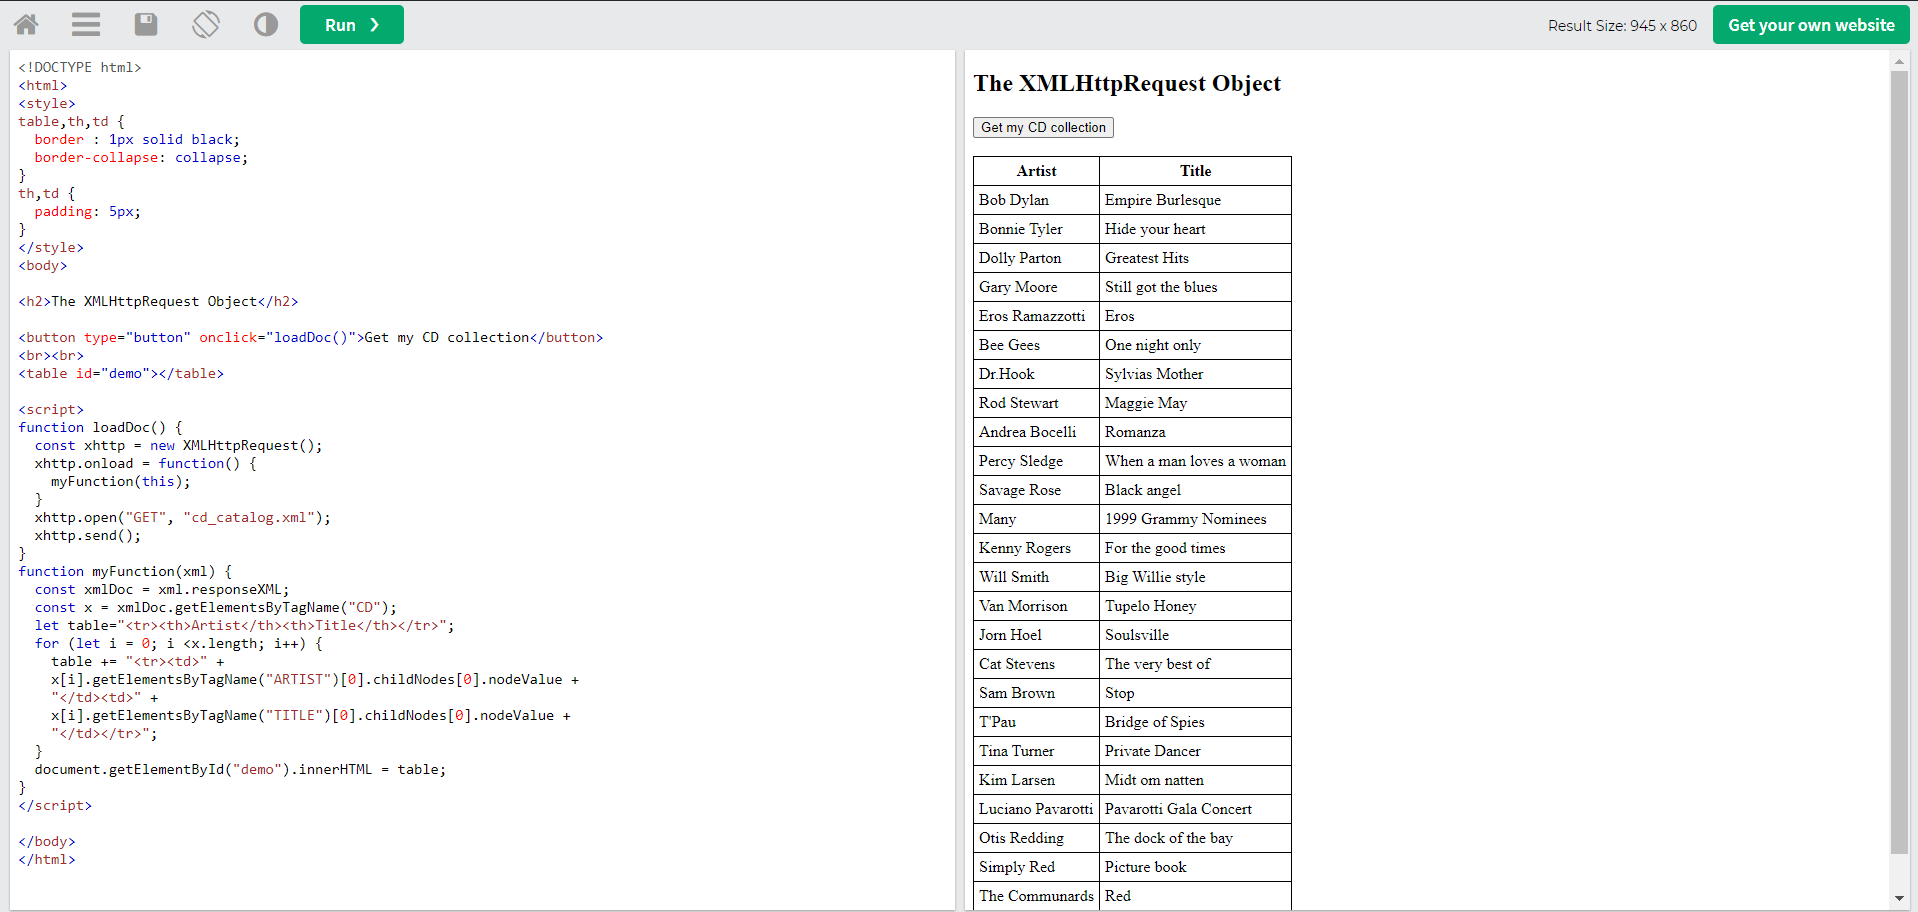
\includegraphics[width=1\textwidth,keepaspectratio]{img/ejemplo27.png}
			\caption{Ejemplo 2}
		\end{figure}
		\newpage
		\item \textbf{Retrieve Server Data with PHP and ASP}
		\begin{figure}[H]
			\centering
			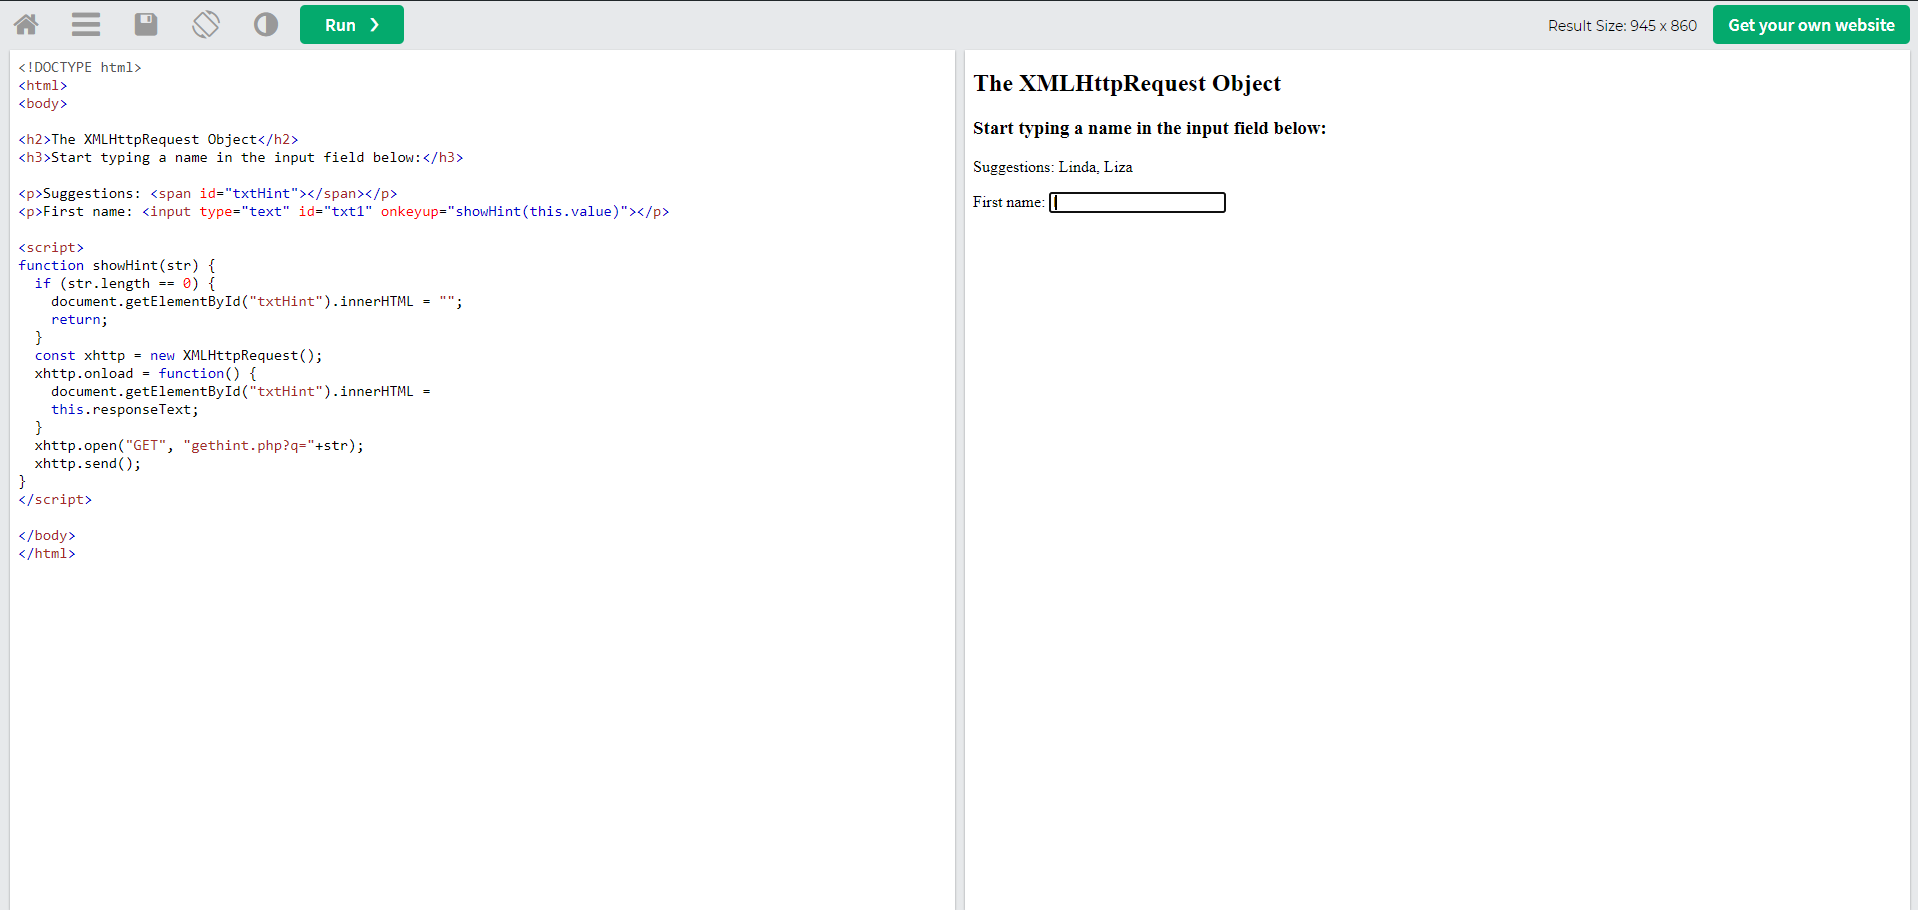
\includegraphics[width=1\textwidth,keepaspectratio]{img/ejemplo28.png}
			\caption{Ejemplo 1}
		\end{figure}
		\begin{figure}[H]
			\centering
			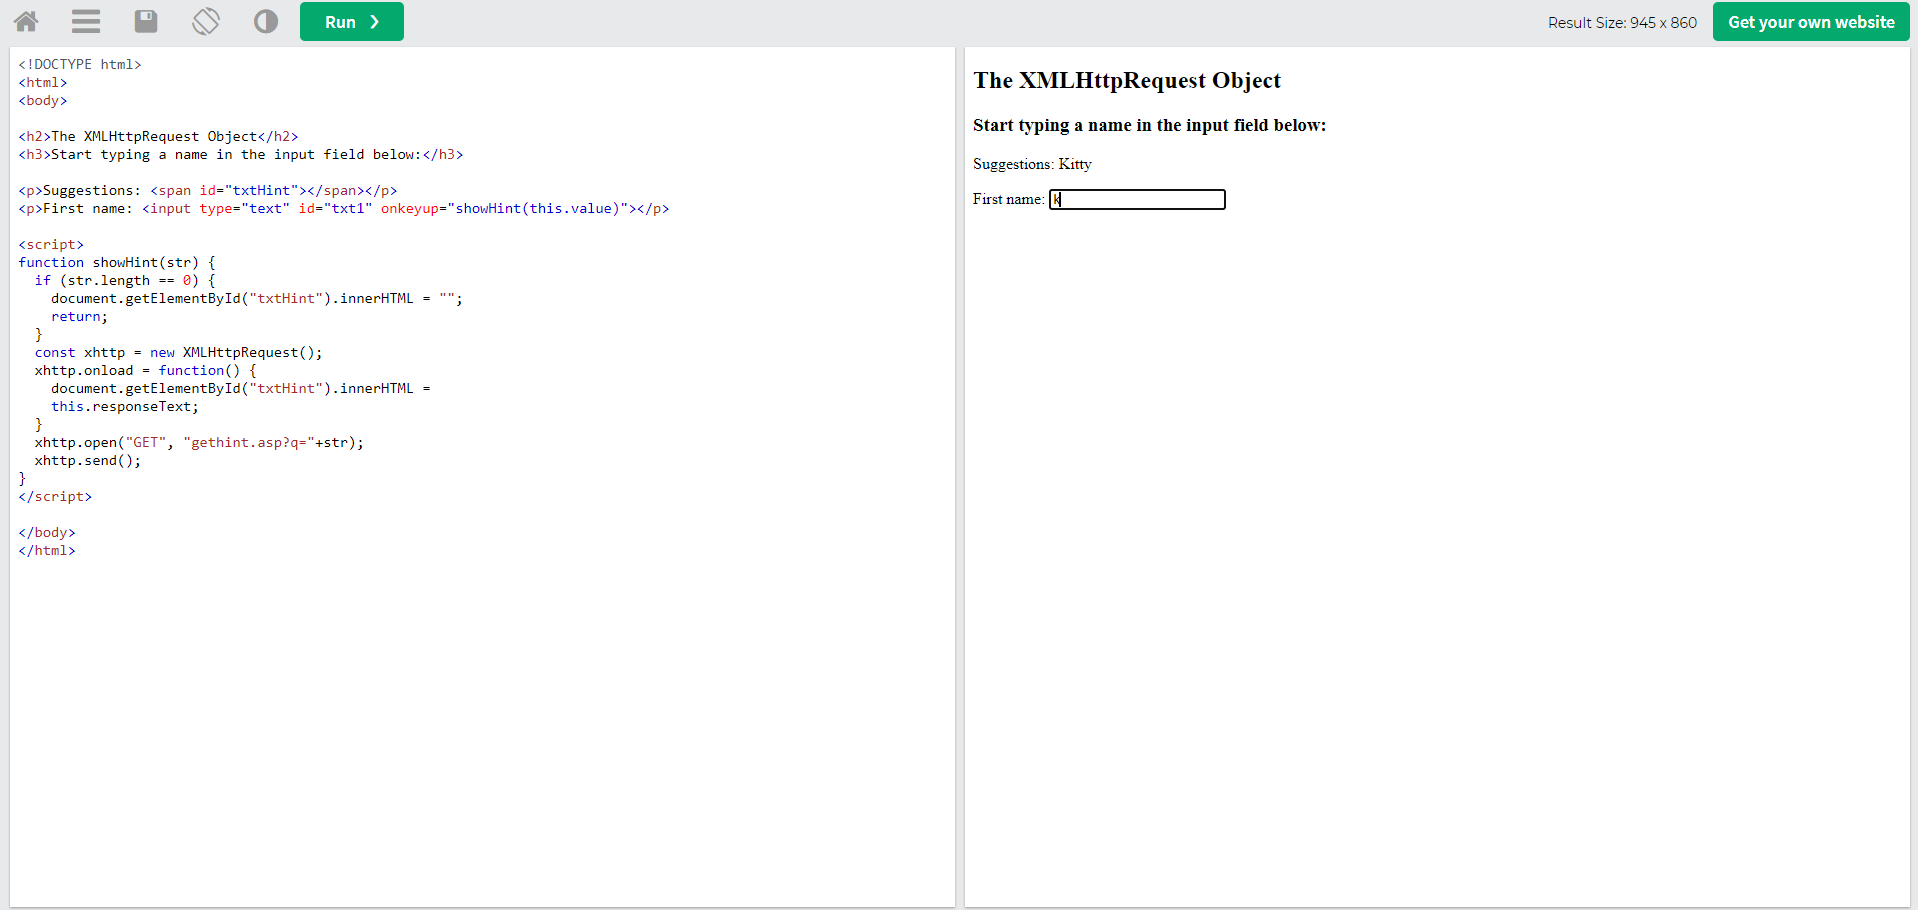
\includegraphics[width=1\textwidth,keepaspectratio]{img/ejemplo29.png}
			\caption{Ejemplo 2}
		\end{figure}
		\newpage
		\item \textbf{Retrieve Database Information}
		\begin{figure}[H]
			\centering
			\includegraphics[width=1\textwidth,keepaspectratio]{img/ejemplo30.png}
			\caption{Ejemplo 1}
		\end{figure}
		\item \textbf{Ajax Applications}
		\begin{figure}[H]
			\centering
			\includegraphics[width=1\textwidth,keepaspectratio]{img/XML.png}
			\caption{XML}
		\end{figure}
		\newpage
		\begin{figure}[H]
			\centering
			\includegraphics[width=1\textwidth,keepaspectratio]{img/ejemplo31.png}
			\caption{Ejemplo 1}
		\end{figure}
		\begin{figure}[H]
			\centering
			\includegraphics[width=1\textwidth,keepaspectratio]{img/ejemplo32.png}
			\caption{Ejemplo 2}
		\end{figure}
		\newpage
		\begin{figure}[H]
			\centering
			\includegraphics[width=1\textwidth,keepaspectratio]{img/ejemplo33.png}
			\caption{Ejemplo 3}
		\end{figure}
		\begin{figure}[H]
			\centering
			\includegraphics[width=1\textwidth,keepaspectratio]{img/ejemplo34.png}
			\caption{Ejemplo 4}
		\end{figure}
	\end{itemize}
%%%%%%%%%%%%%%%%%%%%
    \newpage
	\subsection{Uso de Xampp}
	\begin{itemize}
		\item Proporciona un entorno de servidor local que te permite desarrollar y probar aplicaciones web antes de publicarlas en un servidor web en producción. Usado para los ejercicios 4 - 8.
		\begin{figure}[H]
			\centering
			\includegraphics[width=1\textwidth,keepaspectratio]{img/xampp.png}
			\caption{Xampp}
		\end{figure}
	\end{itemize}
%%%%%%%%%%%%%%%%%%%%
	\subsection{Uso de Node.js}
	\begin{itemize}
		\item Es una plataforma que permite ejecutar código JavaScript del lado del servidor, ofreciendo un entorno altamente escalable y eficiente para el desarrollo de aplicaciones web modernas. Usado para la página web Markdown y del ejercicio 1 - 3
	\end{itemize}
	\subsubsection{Instalación}
	Al descargar el installer, solo seguir los pasos correspondientes.
	\begin{figure}[H]
		\centering
		\includegraphics[width=1\textwidth,keepaspectratio]{img/node.png}
		\caption{Instalación Node.js}
	\end{figure}
%%%%%%%%%%%%%%%%%%%%
	\subsection{Investigación sobre Chart.js}
	\subsubsection{Página Oficial}
	\begin{figure}[H]
		\centering
		\includegraphics[width=1\textwidth,keepaspectratio]{img/Chart_O.png}
		\caption{Chart.js}
	\end{figure}
	\subsubsection{Documentación}
	\begin{figure}[H]
		\centering
		\includegraphics[width=1\textwidth,keepaspectratio]{img/Chart.png}
		\caption{Chart.js DOC}
	\end{figure}
%%%%%%%%%%%%%%%%%%
	\subsection{EJERCICIOS}
	\subsubsection{Ejercicio 1}
	\begin{itemize}
		\item textbf{Script}
		\begin{figure}[H]
			\centering
			\includegraphics[width=1\textwidth,keepaspectratio]{img/Script1.png}
			\caption{Script 1}
		\end{figure}
		\newpage
		\item \textbf{Ejecución}
		\begin{figure}[H]
			\centering
			\includegraphics[width=1\textwidth,keepaspectratio]{img/Ejecucion1.png}
			\caption{Ejercicio 1}
		\end{figure}
	\end{itemize}
%%%%%%%%%%%%%%%%%%%%
    \subsubsection{Ejercicio 2}
    \begin{itemize}
    	\item \textbf{Script}
    	\begin{figure}[H]
    		\centering
    		\includegraphics[width=1\textwidth,keepaspectratio]{img/Script2.png}
    		\caption{Script 2}
    	\end{figure}
    	\newpage
    	\item \textbf{Ejecución}
    	\begin{figure}[H]
    		\centering
    		\includegraphics[width=1\textwidth,keepaspectratio]{img/Ejecucion2.png}
    		\caption{Ejercicio 2}
    	\end{figure}
    \end{itemize}
%%%%%%%%%%%%%%%%%%%%
 	\newpage
    \subsubsection{Ejercicio 3}
	\begin{itemize}
		\item \textbf{Script}
		\begin{figure}[H]
			\centering
			\includegraphics[width=1\textwidth,keepaspectratio]{img/Script3.png}
			\caption{Script 3}
		\end{figure}
		\newpage
		\item \textbf{Ejecución}
		\begin{figure}[H]
			\centering
			\includegraphics[width=1\textwidth,keepaspectratio]{img/Ejecucion3.png}
			\caption{Ejercicio 3}
		\end{figure}
	\end{itemize}
%%%%%%%%%%%%%%%%%%%%
    \subsubsection{Ejercicio 4}
	\begin{itemize}
		\item \textbf{HTML}
		\begin{figure}[H]
			\centering
			\includegraphics[width=1\textwidth,keepaspectratio]{img/html4.png}
			\caption{HTML}
		\end{figure}
		\newpage
		\item \textbf{Script}
		\begin{figure}[H]
			\centering
			\includegraphics[width=1\textwidth,keepaspectratio]{img/Script4.png}
			\caption{Script 4}
		\end{figure}
		\newpage
		\item \textbf{Ejecución}
		\begin{figure}[H]
			\centering
			\includegraphics[width=1\textwidth,keepaspectratio]{img/Ejecucion4.png}
			\caption{Ejercicio 4}
		\end{figure}
	\end{itemize}
%%%%%%%%%%%%%%%%%%%%
	\subsubsection{Ejercicio 5}
	\begin{itemize}
		\item \textbf{comparasion 1}
		\begin{itemize}
			\item \textbf{HTML}
			\begin{figure}[H]
				\centering
				\includegraphics[width=1\textwidth,keepaspectratio]{img/html5.png}
				\caption{HTML 5}
			\end{figure}
			\newpage
			\item \textbf{Script}
			\begin{figure}[H]
				\centering
				\includegraphics[width=1\textwidth,keepaspectratio]{img/Script5-1.png}
				\caption{Script 5 - 1}
			\end{figure}
			\newpage
			\item \textbf{Ejecución}
			\begin{figure}[H]
				\centering
				\includegraphics[width=1\textwidth,keepaspectratio]{img/Ejecucion5-1.png}
				\caption{Ejercicio 5 - 1}
			\end{figure}
		\end{itemize}
		\item \textbf{comparasion 2}
		\begin{itemize}
			\item \textbf{HTML}
			\begin{figure}[H]
				\centering
				\includegraphics[width=1\textwidth,keepaspectratio]{img/html5.png}
				\caption{HTML 5}
			\end{figure}
			\newpage
			\item \textbf{Script}
			\begin{figure}[H]
				\centering
				\includegraphics[width=1\textwidth,keepaspectratio]{img/Script5-2.png}
				\caption{Script 5 - 2}
			\end{figure}
			\newpage
			\item \textbf{Ejecución}
			\begin{figure}[H]
				\centering
				\includegraphics[width=1\textwidth,keepaspectratio]{img/Ejecucion5-2.png}
				\caption{Ejercicio 5 - 2}
			\end{figure}
		\end{itemize}
		\item \textbf{comparasion 3}
		\begin{itemize}
			\item \textbf{HTML}
			\begin{figure}[H]
				\centering
				\includegraphics[width=1\textwidth,keepaspectratio]{img/html5.png}
				\caption{HTML 5}
			\end{figure}
			\newpage
			\item \textbf{Script}
			\begin{figure}[H]
				\centering
				\includegraphics[width=1\textwidth,keepaspectratio]{img/Script5-3.png}
				\caption{Script 5 - 3}
			\end{figure}
			\newpage
			\item \textbf{Ejecución}
			\begin{figure}[H]
				\centering
				\includegraphics[width=1\textwidth,keepaspectratio]{img/Ejecucion5-3.png}
				\caption{Ejercicio 5 - 3}
			\end{figure}
		\end{itemize}
		\item \textbf{comparasion 4}
		\begin{itemize}
			\item \textbf{HTML}
			\begin{figure}[H]
				\centering
				\includegraphics[width=1\textwidth,keepaspectratio]{img/html5.png}
				\caption{HTML 5}
			\end{figure}
			\newpage
			\item \textbf{Script}
			\begin{figure}[H]
				\centering
				\includegraphics[width=1\textwidth,keepaspectratio]{img/Script5-4.png}
				\caption{Script 5 - 4}
			\end{figure}
			\newpage
			\item \textbf{Ejecución}
			\begin{figure}[H]
				\centering
				\includegraphics[width=1\textwidth,keepaspectratio]{img/Ejecucion5-4.png}
				\caption{Ejercicio 5 - 4}
			\end{figure}
		\end{itemize}
	\end{itemize}
%%%%%%%%%%%%%%%%%%%%
	\subsubsection{Ejercicio 6}
	\begin{itemize}
		\item \textbf{HTML}
		\begin{figure}[H]
			\centering
			\includegraphics[width=1\textwidth,keepaspectratio]{img/html6.png}
			\caption{HTML 6}
		\end{figure}
		\newpage
		\item \textbf{Script}
		\begin{figure}[H]
			\centering
			\includegraphics[width=1\textwidth,keepaspectratio]{img/Script6-1.png}
			\caption{Script 6 - 1}
		\end{figure}
		\begin{figure}[H]
			\centering
			\includegraphics[width=1\textwidth,keepaspectratio]{img/Script6-2.png}
			\caption{Script 6 - 2}
		\end{figure}
		\item \textbf{Ejecución}
		\begin{figure}[H]
			\centering
			\includegraphics[width=1\textwidth,keepaspectratio]{img/Ejecucion6.png}
			\caption{Ejercicio 6}
		\end{figure}
	\end{itemize}
%%%%%%%%%%%%%%%%%%%%
	\newpage
	\subsubsection{Ejercicio 7}
	\begin{itemize}
		\item \textbf{HTML}
		\begin{figure}[H]
			\centering
			\includegraphics[width=1\textwidth,keepaspectratio]{img/html7-1.png}
			\caption{HTML 7 - 1}
		\end{figure}
		\begin{figure}[H]
			\centering
			\includegraphics[width=1\textwidth,keepaspectratio]{img/html7-2.png}
			\caption{HTML 7 - 2}
		\end{figure}
		\newpage
		\item \textbf{Script}
		\begin{figure}[H]
			\centering
			\includegraphics[width=1\textwidth,keepaspectratio]{img/Script7-1.png}
			\caption{Script 7-1}
		\end{figure}
		\begin{figure}[H]
			\centering
			\includegraphics[width=1\textwidth,keepaspectratio]{img/Script7-2.png}
			\caption{Script 7 - 2}
		\end{figure}
		\item \textbf{Ejecución}
		\begin{figure}[H]
			\centering
			\includegraphics[width=1\textwidth,keepaspectratio]{img/Ejecucion7.png}
			\caption{Ejercicio 7}
		\end{figure}
	\end{itemize}
%%%%%%%%%%%%%%%%%%%%
	\subsubsection{Ejercicio 8}
	\begin{itemize}
		\item \textbf{HTML}
		\begin{figure}[H]
			\centering
			\includegraphics[width=1\textwidth,keepaspectratio]{img/html8.png}
			\caption{HTML 8}
		\end{figure}
		\item \textbf{Script}
		\begin{figure}[H]
			\centering
			\includegraphics[width=0.8\textwidth,keepaspectratio]{img/Script8-1.png}
			\caption{Script 8 - 1}
		\end{figure}
		\begin{figure}[H]
			\centering
			\includegraphics[width=1\textwidth,keepaspectratio]{img/Script8-2.png}
			\caption{Script 8 - 2}
		\end{figure}
		\item \textbf{Ejecución}
		\begin{figure}[H]
			\centering
			\includegraphics[width=1\textwidth,keepaspectratio]{img/Ejecucion8.png}
			\caption{Ejercicio 8}
		\end{figure}
	\end{itemize}
%%%%%%%%%%%%%%%%%%%%
	\subsubsection{CSS}
	\begin{itemize}
		\item \textbf{CSS}
		\begin{figure}[H]
			\centering
			\includegraphics[width=1\textwidth,keepaspectratio]{img/css1.png}
			\caption{Estilos ejercicio 4 - 8}
		\end{figure}
	\end{itemize}
%%%%%%%%%%%%%%%%%%%%
	\subsection{Ejercicio Propuesto: Página Web - Markdown}
	\begin{itemize}
		\item \textbf{HTML}
		\begin{figure}[H]
			\centering
			\includegraphics[width=1\textwidth,keepaspectratio]{img/html.png}
			\caption{HTML }
		\end{figure}
		\item \textbf{Script 1}
		\begin{figure}[H]
			\centering
			\includegraphics[width=1\textwidth,keepaspectratio]{img/Scriptindex.png}
			\caption{Script index.js 1}
		\end{figure}
		\begin{figure}[H]
			\centering
			\includegraphics[width=1\textwidth,keepaspectratio]{img/Scriptapp1.png}
			\caption{Script app.js 2 - 1}
		\end{figure}
		\begin{figure}[H]
			\centering
			\includegraphics[width=1\textwidth,keepaspectratio]{img/Scriptapp2.png}
			\caption{Script app.js 2 - 2}
		\end{figure}
		\item \textbf{Ejecución}
		\begin{figure}[H]
			\centering
			\includegraphics[width=1\textwidth,keepaspectratio]{img/web1.png}
			\caption{Servidor Activado}
		\end{figure}
		\begin{figure}[H]
			\centering
			\includegraphics[width=1\textwidth,keepaspectratio]{img/web2.png}
			\caption{Botón Enviar}
		\end{figure}
		\begin{figure}[H]
			\centering
			\includegraphics[width=1\textwidth,keepaspectratio]{img/web3.png}
			\caption{Botón Listar}
		\end{figure}
		\begin{figure}[H]
			\centering
			\includegraphics[width=1\textwidth,keepaspectratio]{img/web4.png}
			\caption{Mostrar página de la Lista}
		\end{figure}
		\begin{figure}[H]
			\centering
			\includegraphics[width=1\textwidth,keepaspectratio]{img/web5.png}
			\caption{console.log}
		\end{figure}
		\item \textbf{CSS}
		\begin{figure}[H]
			\centering
			\includegraphics[width=1\textwidth,keepaspectratio]{img/css2.png}
			\caption{Estilos de Página Markdown}
		\end{figure}
	\end{itemize}
%%%%%%%%%%%%%%%%%%%%

    \subsection{Uso de GitHub}
	\subsubsection{Cuenta de GitHub}
	\begin{figure}[H]
		\centering
		\includegraphics[width=0.95\textwidth,keepaspectratio]{img/usuario.png}
		\caption{Usuario}
	\end{figure}
%%%%%%%%%%%%%%%%%%%%
	\subsection{Creación de un Nuevo Repositorio}
	\subsubsection{Implementación de Readme.md}
	\begin{figure}[H]
		\centering
		\includegraphics[width=0.95\textwidth,keepaspectratio]{img/readme.png}
		\caption{Readme.md}
	\end{figure}
%%%%%%%%%%%%%%%%%%%%
	\subsubsection{Registro de cambios en mi código}
	\begin{itemize}
		\item \textbf{Commits}
		\begin{figure}[H]
			\centering
			\includegraphics[width=0.94\textwidth,keepaspectratio]{img/Commits.png}
			\caption{Commits}
		\end{figure}
	\end{itemize}
	
%%%%%%%%%%%%%%%%%%%%
	\subsubsection{Repositorio}
	\begin{figure}[H]
		\centering
		\includegraphics[width=1\textwidth,keepaspectratio]{img/Repositorio.png}
		\caption{Repositorio}
	\end{figure}
%%%%%%%%%%%%%%%%%%%%
	\subsubsection{Proyecto compartido con el profesor de github}
	\begin{figure}[H]
		\centering
		\includegraphics[width=1\textwidth,keepaspectratio]{img/Compartir.png}
		\caption{Compartir con el Profesor}
	\end{figure}
	\newpage
	\subsection{\textcolor{red}{Rúbrica para el contenido del Informe y demostración}}
	\begin{itemize}			
		\item El alumno debe marcar o dejar en blanco en celdas de la columna \textbf{Checklist} si cumplio con el ítem correspondiente.
		\item Si un alumno supera la fecha de entrega,  su calificación será sobre la nota mínima aprobada, siempre y cuando cumpla con todos lo items.
		\item El alumno debe autocalificarse en la columna \textbf{Estudiante} de acuerdo a la siguiente tabla:
	
		\begin{table}[ht]
			\caption{Niveles de desempeño}
			\begin{center}
			\begin{tabular}{ccccc}
    			\hline
    			 & \multicolumn{4}{c}{Nivel}\\
    			\cline{1-5}
    			\textbf{Puntos} & Insatisfactorio 25\%& En Proceso 50\% & Satisfactorio 75\% & Sobresaliente 100\%\\
    			\textbf{2.0}&0.5&1.0&1.5&2.0\\
    			\textbf{4.0}&1.0&2.0&3.0&4.0\\
    		\hline
			\end{tabular}
		\end{center}
	\end{table}	
	

	\end{itemize}

 
	
	\begin{table}[H]
		\caption{Rúbrica para contenido del Informe y demostración}
		\setlength{\tabcolsep}{0.5em} % for the horizontal padding
		{\renewcommand{\arraystretch}{1.5}% for the vertical padding
		%\begin{center}
		\begin{tabular}{|p{2.7cm}|p{7cm}|x{1.3cm}|p{1.2cm}|p{1.5cm}|p{1.1cm}|}
			\hline
    		\multicolumn{2}{|c|}{Contenido y demostración} & Puntos & Checklist & Estudiante & Profesor\\
			\hline
			\textbf{1. GitHub} & Hay enlace URL activo del directorio para el  laboratorio hacia su repositorio GitHub con código fuente terminado y fácil de revisar. &2 &X &2 & \\ 
			\hline
			\textbf{2. Commits} &  Hay capturas de pantalla de los commits más importantes con sus explicaciones detalladas. (El profesor puede preguntar para refrendar calificación). &4 &X &4 & \\ 
			\hline 
			\textbf{3. Código fuente} &  Hay porciones de código fuente importantes con numeración y explicaciones detalladas de sus funciones. &2 &X &2 & \\ 
			\hline 
			\textbf{4. Ejecución} & Se incluyen ejecuciones/pruebas del código fuente  explicadas gradualmente. &2 &X &2 & \\ 
			\hline			
			\textbf{5. Pregunta} & Se responde con completitud a la pregunta formulada en la tarea.  (El profesor puede preguntar para refrendar calificación).  &2 &X &2 & \\ 
			\hline	
			\textbf{6. Fechas} & Las fechas de modificación del código fuente estan dentro de los plazos de fecha de entrega establecidos. &2 &X &2 & \\ 
			\hline 
			\textbf{7. Ortografía} & El documento no muestra errores ortográficos. &2 &X &2 & \\ 
			\hline 
			\textbf{8. Madurez} & El Informe muestra de manera general una evolución de la madurez del código fuente,  explicaciones puntuales pero precisas y un acabado impecable.   (El profesor puede preguntar para refrendar calificación).  &4 &X &4 & \\ 
			\hline
			\multicolumn{2}{|c|}{\textbf{Total}} &20 & &20 & \\ 
			\hline
		\end{tabular}
		%\end{center}
		%\label{tab:multicol}
		}
	\end{table}


%%%%%%%%%%%%%%%%%%%%%%%%%%%%%%%%%%%%%%%%%%%%%%%%%%%%%%%%%%%%%%%%%%%
	\newpage
% 

    \section{Referencias}
    \begin{itemize}	
        \item \url{https://www.chartjs.org/}
        \item \url{https://www.chartjs.org/docs/latest/}
        \item \url{https://git-scm.com/doc}
        \item \url{https://www.w3schools.com/js/default.asp}
	\end{itemize}

 
%\clearpage
%\bibliographystyle{apalike}
%\bibliographystyle{IEEEtranN}
%\bibliography{bibliography}
			
\end{document}